\documentclass[12pt, letter]{report}
\usepackage{mathptmx}
\usepackage{titlesec}
\usepackage{graphicx}
\usepackage{graphics}
\usepackage{ragged2e}
\usepackage{setspace}
\usepackage[toc, page]{appendix}
\usepackage{amssymb, amsmath}
\usepackage{import}
\usepackage{svg}
\usepackage{xcolor}
\usepackage{siunitx}
\usepackage{caption}
\usepackage{subcaption}
\usepackage{booktabs}
\usepackage{listings}
\usepackage[hidelinks]{hyperref}
\usepackage{xcolor}
\usepackage{longtable,tabularx}
\usepackage[bottom=25mm, top=25mm, left=20mm, right=20mm]{geometry}
\usepackage{pdfpages}
\usepackage{multirow}
\usepackage{fancyhdr}
\usepackage{subcaption}
\usepackage{tocloft}
\usepackage{float}
\usepackage{verbatim}
\usepackage{minted}

%tikzpicture
\usepackage{tikz}
\usepackage{scalerel}
\usepackage{pict2e}
\usepackage{tkz-euclide}
\usetikzlibrary{calc}
\usetikzlibrary{patterns,arrows.meta}
\usetikzlibrary{shadows}
\usetikzlibrary{external}

%pgfplots
\usepackage{pgfplots}
\pgfplotsset{compat=newest}
\usepgfplotslibrary{statistics}
\usepgfplotslibrary{fillbetween}

%FOR PART B
\usepackage{gensymb} % for \degree command

\renewcommand{\chaptername}{Section}           % Changes level 1 heading from chapter -> part

% Change the style for Table of Contents, Figures and Tables
\renewcommand{\cfttoctitlefont}{\sffamily\large\bfseries}
\renewcommand{\cftloftitlefont}{\sffamily\large\bfseries}
\renewcommand{\cftlottitlefont}{\sffamily\large\bfseries}

\setstretch{1.1}
%%%%%%%%%%%%%%%%%%%%%%%%%%%%%%%%%%%%%%%%%%%%%%%%%%%%%%%%%%%%%%%%%%%%%%%%%%%%%%%%%%%%%%%%%%
%               FORMATTING FOR PRE TECHNICAL CONTENT              %
%%%%%%%%%%%%%%%%%%%%%%%%%%%%%%%%%%%%%%%%%%%%%%%%%%%%%%%%%%%%%%%%%%%%%%%%%%%%%%%%%%%%%%%%%%

\titleformat{\section}
  {\normalfont\centering\sffamily\bfseries}{\thesection}{1em}{}

%%%%%%%%%%%%%%%%%%%%%%%%%%%%%%%%%%%%%%%%%%%%%%%%%%%%%%%%%%%%%%%%%%%%%%%%%%%%%%%%%%%%%%%%%%
%               BEGINNING OF DOCUMENT              %
%%%%%%%%%%%%%%%%%%%%%%%%%%%%%%%%%%%%%%%%%%%%%%%%%%%%%%%%%%%%%%%%%%%%%%%%%%%%%%%%%%%%%%%%%%
\begin{document}
%%%%%%%%%%%%%%%%%%%%%%%%%%%%%%%%%%%%%%%%%%%%%%%%%%%%%%%%%%%%%%%%%%%%%%%%%%%%%%%%%%%%%%%%%%
%               TITLE PAGE              %
%%%%%%%%%%%%%%%%%%%%%%%%%%%%%%%%%%%%%%%%%%%%%%%%%%%%%%%%%%%%%%%%%%%%%%%%%%%%%%%%%%%%%%%%%%
\begingroup
\let\newpage\relax 
\title{\huge{{Design Report\\ \textbf{Gas Turbine Design}}}}
\vspace{200pt}
\date{\today}
\maketitle
\thispagestyle{empty}
\endgroup 

\vspace{90pt}
\begin{center}
  %\author{\vspace{10pt} Paramvir Singh Lobana (40119637) \\
  %Rafal-Michal Czuprynski (26661440)\\
  %Anne Blouin (40173750) \\
  %Muhammad Saghir (40112152) \\
  %Zac Heit (40124271) \\
  %Andrew Young (40110619) \\
  %Gabriel Fraser (40131870) \\}
  
\end{center}
\vspace{20pt}
\begin{center}

\includegraphics[scale=0.04]{figures/logo.png}
\end{center}
\begin{center}
\large Department of Mechanical, Industrial and Aerospace Engineering, \\ Concordia University \\ Montreal, QC, Canada
\end{center}
\clearpage



\begin{titlepage}
    \centering
    \vspace*{2cm}
    {\LARGE \textbf{Technical Report}}\par
    \vspace{2cm}
    {\Huge \textbf{Core Engine Design}}\par
\vspace{2cm}
    {\Large Date: \today}\par
    \vspace{2cm}


    \begin{center}

\includegraphics[scale=0.25]{figures/named_logo.png}
\end{center}
    \vspace{0.5cm}
    {\large Collaborative Innovation Department}\par
    \vspace{0.5cm}
    {\large Address: 1455 Blvd. De Maisonneuve Ouest\\
     Montreal, Quebec H3G 1M8}\par
    \vspace{0.5cm}
    {\large Contact: info@aerospec.com}\par
    \vfill
    \vspace{1cm}
    {\small This report is submitted in partial fulfillment of the requirements for the partnership agreement with Pratt \& Whitney Canada.}
\end{titlepage}

\clearpage

%%%%%%%%%%%%%%%%%%%%%%%%%%%%%%%%%%%%%%%%%%%%%%%%%%%%%%%%%%%%%%%%%%%%%%%%%%%%%%%%%%%%%%%%%%
%               END OF TITLE PAGE              %
%               PREFACE or INTRO              %
%%%%%%%%%%%%%%%%%%%%%%%%%%%%%%%%%%%%%%%%%%%%%%%%%%%%%%%%%%%%%%%%%%%%%%%%%%%%%%%%%%%%%%%%%%
\pagenumbering{roman}
%\section*{Preface or Abstract}
%\addcontentsline{toc}{section}{Preface} 
% Discuss about project 
% How the team was divided. Roles and responsibilities.


\clearpage
%%%%%%%%%%%%%%%%%%%%%%%%%%%%%%%%%%%%%%%%%%%%%%%%%%%%%%%%%%%%%%%%%%%%%%%%%%%%%%%%%%%%%%%%%%


\tableofcontents

\pagebreak
\listoffigures
\addcontentsline{toc}{section}{List of Figures}
\listoftables
\addcontentsline{toc}{section}{List of Tables}
\pagebreak


\section*{Nomenclature - Compressor}
\addcontentsline{toc}{section}{Nomenclature - Compressor}
\begin{longtable*}{@{}l @{\quad  -  \quad} l@{}}

$N_s$ & Centrifugal Specific Speed \\
${\rho}$ & Density \\
$Q$ & Volume Flow \\
$\Delta h_{0,\text{is}}$ & Isentropic Enthalpy Rise \\
$N$ &  Rotational Speed\\
$w$  &  Rotational Speed\\
$r$ & Radius \\
$L$ &  Compressor Length\\
$b$ & Height \\
$N_b$ & Number of Blade\\
$T$ & Temperature\\
$\dot m$ & Mass Flow Rate\\
$C$ & Absolute Velocity\\
$\alpha$ & Swirl Angle \\
$U$ & Blade's Velocity\\
$W$ & Relative Velocity\\
$\beta$ & Back Sweep Angle\\
$M_{rel}$ & Relative Mach Number\\
$\theta$ & Flow Turning Angle\\
$W_{thermo}$ & Thermo Work\\
$\sigma$ & Slip Factor\\
$A$ & Area\\
$i$ & Incidence Angle\\
$\beta ^*$ & Metal's Angle\\
$P$ & Pressure\\

\end{longtable*}
\begin{center}
   \textbf{Subscripts} \\
\end{center}

\begin{longtable*}{@{}l @{\quad  -  \quad} l@{}}

$1$ & At the Impeller's Inlet\\
$2$ & At Impeller's Outlet, At the Diffuser's Inlet \\
3 & At Diffuser's Outlet\\
$h$ & At the Hub\\
$m$ & At the Mean\\
$sh$ & At the Shroud\\
$partA$ & From Part A\\
$x$ & Axial's Direction\\
$r$ & Axial's Direction\\

\end{longtable*}

\vspace{20pt}

\section*{Nomenclature - Turbine}
\addcontentsline{toc}{section}{Nomenclature - Turbine}

\begin{longtable*}{@{}l @{\quad  -  \quad} l@{}}

$h$ & Blade Height \\
$c_{true}$ & True Chord \\
$c_a$ & Axial Chord \\
$C_L$ & Lift Coefficient \\
$f_{AR}$ & Aspect Ratio Function \\
%$f_{Re}$ & Reynold's Number Correction Factor \\
$K_1, K_2, K_3, K^*_p, K_{sh}, K^*_s, K_{accl}$ & Correction Loss Factors \\
$K_T, K_p, K_s, K_{TE}$ & Loss Coefficients \\
$s$ & Pitch \\
$o$ & Throat Opening \\
$\Phi$ & Stagger Angle \\
$R$ & Reaction \\
$\psi$ & Stage Loading \\
$\phi$ & Flow Coefficient \\
$U_{mean, hub, tip}$ & Blade Speed at Mean, Hub, Tip \\
$AN^2$ & Annulus Area x Rotational Speed Squared \\
$\omega$ & Angular Velocity \\
$\rho$ & Density  \\
$P_{0, rel}$ & Relative Stagnation Pressure \\
$M_{hub}$ & Absolute Mach Number at Hub  \\
$M_{rel}$ & Relative Mach Number \\
$M_{abs}$ & Absolute Mach Number \\
$T_0$ & Stagnation Temperature  \\
$P_0$ & Stagnation Pressure  \\
$\dot{m}$ & Mass Flow Rate  \\
$P$ & Static Pressure   \\
$T$ & Static Temperature  \\
$C$ & Absolute Velocity \\
$C_w$ & Tangential Velocity \\
$C_a$ & Axial Velocity \\
$\alpha$ & Absolute/Relative Flow Angle  \\
$\beta$ & Metal Angle \\
$V$ & Relative Velocity \\
$V_w$ & Tangential Relative Velocity \\
$A$ & Area \\
$r_{hub, mean, tip}$ & Radius at Hub, Meanline, Tip \\
$\eta_{tt}$ & Total-to-Total Turbine Efficiency \\
$\eta_o$ & Efficiency at 0 Tip Clearance \\ 
$N$ & Number of Vanes/Blades

\end{longtable*}

\pagebreak



%%%%%%%%%%%%%%%%%%%%%%%%%%%%%%%%%%%%%%%%%%%%%%%%%%%%%%%%%%%%%%%%%%%%%%%%%%%%%%%%%%%%%%%%%%
%               FORMATTING FOR TECHNICAL CONTENT              %
%%%%%%%%%%%%%%%%%%%%%%%%%%%%%%%%%%%%%%%%%%%%%%%%%%%%%%%%%%%%%%%%%%%%%%%%%%%%%%%%%%%%%%%%%%
\titleformat{\chapter}[display]
  {\normalfont\huge\bfseries\sffamily}{\chaptertitlename\ \thechapter}{20pt}{\Huge}
\titleformat{\section}
  {\normalfont\sffamily\bfseries}{\thesection}{1em}{}
\titleformat{\subsection}
  {\normalfont\sffamily\bfseries}{\thesubsection}{1em}{}
\titleformat{\subsubsection}
  {\normalfont\sffamily}{\thesubsubsection}{1em}{}

%%%%%%%%%%%%%%%%%%%%%%%%%%%%%%%%%%%%%%%%%%%%%%%%%%%%%%%%%%%%%%%%%%%%%%%%%%%%%%%%%%%%%%%%%
% DO NOT CHANGE ANYTHING BEFORE THIS IN THE CODE
\pagenumbering{arabic}
\setcounter{page}{1}
%%%%%%%%%%%%%%%%%%%%%%%%%%%%%%%%%%%%%%%%%%%%%%%%%%%%%%%%%%%%%%%%%%%%%%%%%%%%%%%%%%%%%%%%%%
%%%%%%%%%%%%%%%%%%%%%%%%%%%%%%%%%%%%%%%%%%%%%%%%%%%%%%%%%%%%%%%%%%%%%%%%%%%%%%%%%%%%%%%%%%
%               BEGINNING OF TECHNICAL CONTENT              %
%%%%%%%%%%%%%%%%%%%%%%%%%%%%%%%%%%%%%%%%%%%%%%%%%%%%%%%%%%%%%%%%%%%%%%%%%%%%%%%%%%%%%%%%%%
%%%%%%%%%%%%%%%%%%%%%%%%%%%%%%%%%%%%%%%%%%%%%%%%%%%%%%%%%%%%%%%%%%%%%%%%%%%%%%%%%%%%%%%%%%
%               PART A             %
%%%%%%%%%%%%%%%%%%%%%%%%%%%%%%%%%%%%%%%%%%%%%%%%%%%%%%%%%%%%%%%%%%%%%%%%%%%%%%%%%%%%%%%%%%
%% IMPORTANT -> Part A is hidden for now, to add it to the report, remove the precent sign from the next line:
\chapter{Cycle Calculations} \label{sec:cyclecalcs}
The objective of this technical report is to present a design for a new family of gas turbine engines under a risk-sharing partnership with Pratt \& Whitney Canada.
The turboshaft engine design should have a three shaft arrangement for sea level operation at $74^{o}F$.
The engine features a single-stage low-pressure compressor (LPC) and axial turbine 
(LPT), followed by a centrifugal high-pressure compressor (HPC) and axial 
high-pressure turbine (HPT). The power turbine (PT) drives the helicopter rotor 
through a reduction gearbox. 

The following figure presents the engine schematics along with all the stations.
\vspace{20pt}
\begin{figure}[H]
  \centering
  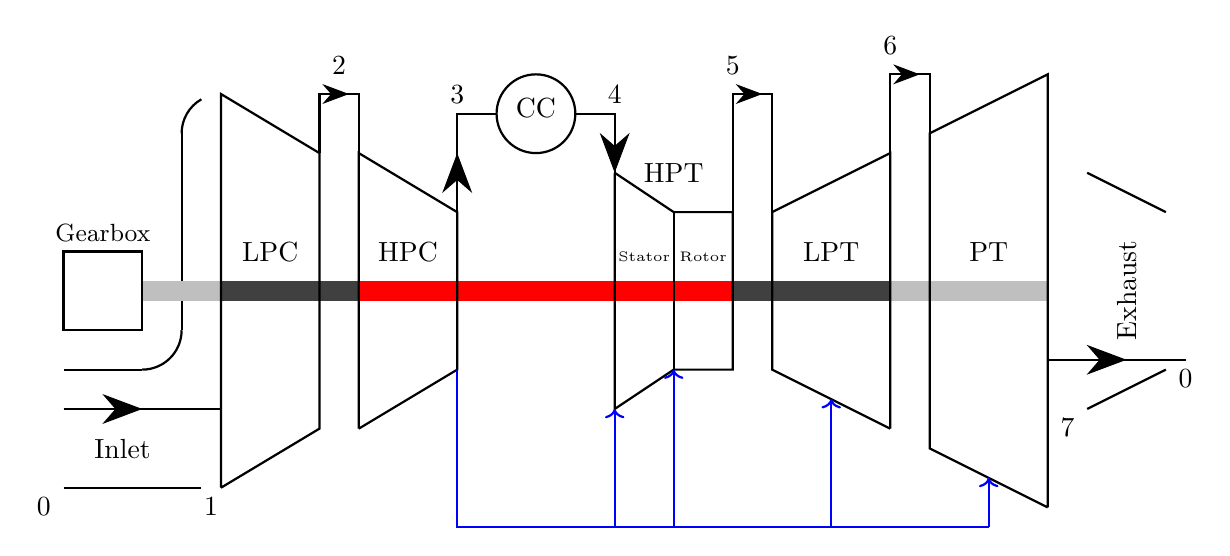
\begin{tikzpicture}[scale=0.5]

%\draw [lightgray](0,0) grid (30, 20);

% Inlet 
\draw [thick] (1, 5) -- (4.5, 5);
\draw [thick] (1, 8) -- (3, 8);
\draw [thick] (3, 8) arc (270:360:1);
\draw [thick] (4, 9) -- (4, 14);
\draw [thick] (4, 14) arc (180:120:1);

% SHAFTS
\fill [lightgray] (26, 9.75) rectangle (3, 10.25); % Power turbine shaft
\fill [darkgray] (22, 9.75) rectangle (5, 10.25); % High Pressure shaft
\fill [red] (8.5, 9.75) rectangle (18, 10.25); % Low Pressure shaft
%==============================================================================================

% Internal Engine Components
\draw [thick] (1, 7) -- (5, 7);
\draw [-{Stealth[scale=3]}] (1, 7) -- (3, 7);
%LPC
\draw [thick] (5,5) -- (5, 15) -- (7.5, 13.5) -- (7.5, 6.5) -- (5,5);
%---------------------
\draw [thick] (7.5, 13.5) -- (7.5, 15) -- (8.5, 15) -- (8.5, 13.5) ;
\draw [-{Stealth[scale=2]}] (7.5, 15) -- (8.25, 15);
%---------------------
%HPC
\draw [thick] (8.5,6.5) -- (8.5, 13.5) -- (11, 12) -- (11, 8) -- (8.5,6.5);

% Combustion Chamber
\draw [thick] (11, 12) -- (11, 14.5) -- (12, 14.5);
\draw [-{Stealth[scale=3]}] (11, 12) -- (11, 13.5);
\draw [thick] (13, 14.5) circle [radius=1];
\draw [thick] (14, 14.5) -- (15, 14.5) -- (15, 12);
\draw [-{Stealth[scale=3]}] (15, 14.5) -- (15, 13);

%HPT
\draw [thick]  (15, 13) -- (15, 7) -- (16.5, 8) -- (18, 8) -- (18, 12) -- (16.5, 12) -- (15, 13);
\draw [thick]  (16.5, 12) -- (16.5, 7);
%---------------------
\draw [thick] (18, 12) -- (18, 15) -- (19, 15) -- (19, 12) ;
\draw [-{Stealth[scale=2]}] (18, 15) -- (18.75, 15);
%---------------------


%LPT
\draw [thick] (22, 6.5) -- (22, 13.5) -- (19, 12) -- (19, 8) -- (22, 6.5);

%---------------------
\draw [thick] (22, 12) -- (22, 15.5) -- (23, 15.5) -- (23, 14) ;
\draw [-{Stealth[scale=2]}] (22, 15.5) -- (22.75, 15.5);
%---------------------

% Power Turbine
\draw [thick] (26,4.5) -- (26, 15.5) -- (23, 14) -- (23, 6) -- (26, 4.5);
\draw [thick] (26, 8.25) -- (29.5, 8.25);
\draw [-{Stealth[scale=3]}] (26, 8.25) -- (28, 8.25);

% Exhaust
\draw [thick] (27, 7) -- (29, 8);
\draw [thick] (27, 13) -- (29, 12);

%==============================================================================================

% Gearbox
\draw [thick] (1, 9) rectangle (3, 11);
\coordinate[label=above: \small{Gearbox}] (Y) at (2, 11);
% Naming


% Compressor
\coordinate[label=above: LPC] (A) at (6.25,10.5);
\coordinate[label=above: HPC] (B) at (9.75,10.5);

% Compressor
\coordinate[label=above: CC] (C) at (13,14.15);

% Turbine
\coordinate[label=above: HPT] (D) at (16.5,12.5);
\coordinate[label=above: \tiny{Stator}] (DA) at (15.75,10.5);
\coordinate[label=above: \tiny{Rotor}] (DB) at (17.25,10.5);



\coordinate[label=above: LPT] (E) at (20.5,10.5);
\coordinate[label=above: PT] (G) at (24.5,10.5);


\coordinate[label=above: Inlet] (H) at (2.5,5.5);
\coordinate[label=above: \rotatebox{90} {Exhaust}] (H) at (28,8.5);

% Stations
\coordinate[label=below: 1] (Y) at (4.75, 5);

\coordinate[label=above: 2] (Y) at (8, 15.25);

\coordinate[label=above: 3] (Y) at (11, 14.5);

\coordinate[label=above: 4] (Y) at (15, 14.5);

\coordinate[label=above: 5] (Y) at (18, 15.25);

\coordinate[label=above: 6] (Y) at (22, 15.75);

\coordinate[label=below: 7] (Y) at (26.5, 7);

\coordinate[label=below: 0] (Y) at (0.5, 5);

\coordinate[label=below: 0] (Y) at (29.5, 8.25);



% Cooling

% HPT VANE
\draw [blue, thick] (11, 8) -- (11, 4) -- (15, 4);
\draw [blue, thick, ->] (15, 4) -- (15, 7);
%HPT DISC
\draw [blue, thick] (15, 4) -- (16.5, 4);
\draw [blue, thick, ->] (16.5, 4) -- (16.5, 8);
% LPT DISC
\draw [blue, thick] (16.5, 4) -- (20.5, 4);
\draw [blue, thick, ->] (20.5, 4) -- (20.5, 7.25);
% PT DISC
\draw [blue, thick] (20.5, 4) -- (24.5, 4);
\draw [blue, thick, ->] (24.5, 4) -- (24.5, 5.25);

\end{tikzpicture}

  \caption{Engine Schematic}
  \label{fig:enter-label}
\end{figure} 

\clearpage

The key engine requirements are summarized in \autoref{tab:enginecharacteristics}.
\begin{table}[H]
    \caption{Engine Characteristics}
    \label{tab:enginecharacteristics}
    \centering
    \begin{tabular}[H]{l l l l}
    \toprule[1pt]
    \multicolumn{2}{c}{\textit{Engine Inlet}}    & \multicolumn{2}{c}{\textit{Compressor}}                    \\
    \midrule
    Inlet Loss     & 1.00 \%              &   Mass Flow                          &  5.21 $kg/sec$  \\
    && LPC PR & 4 \\
    && LPC Target Efficiency & 86.5 \% \\
    && HPC PR & 3 \\
    && HPC Target Efficiency & 85.5 \% \\
    && HPC Bleed Air (exit) & 9 \% \\
    \midrule
    \multicolumn{2}{c}{\textit{Combustor}}    & \multicolumn{2}{c}{\textit{Turbine}}                    \\
    \midrule
    Fuel to Air ratio & 0.02 & HPT Target Efficiency& 83 \%-85 \%\\
    Heating Value & 40007.2 $kJ/kg$ & HPT Vane Cooling Air& 3 \%\\
    Efficiency & 0.99 & HPT Disk Cooling Air& 1.65 \%\\
    Pressure Loss & 1.8 \% &LPT Target Efficiency& 91 \% \\
    RTDF & 5 \% &LPT Disk Cooling Air& 1.1 \%\\
    && ITD loss & 0.6 \% \\
    && PT Target Efficiency & 92 \%\\
    && PT disk cooling air & 1.25 \% \\
    && Exhaust Loss & 2.0 \% \\
    && Exhaust Mach Number & 0.15 \\
    \midrule[1pt]
    \end{tabular}
\end{table} 


This section discusses the method used for the cycle calculations. The calculations for each stage are presented as well.

\section{Inlet}
Since $P_{00} = P_a$ and $T_{00} = T_a$, the pressure drop across the inlet can be calculated as:
$$P_{01} = 0.99 \times P_{00} = 100.311 \; kPa$$
$$T_{01} = 296.483 \; K$$

\section{Low Pressure Compressor} \label{lpc}
The pressure at the LPT exit $(P_{02})$ can be calculated as:
$$P_{02} = PR_{LPC} \times P_{01} = 401.247 \; kPa$$

The temperature can be obtained using the following relation:
\begin{equation}
  T_{02} - T_{01} = \frac{T_{01}}{\eta_{lpc}} \left[  \left( \frac{P_{02}}{P_{01}} \right) ^{(\gamma - 1)/\gamma}  - 1  \right]
\end{equation}

$$T_{02} = 463.059 \; K$$

Therefore, the specific work done for the LPC:
$$W_{LPC} = c_{p, \, air} \times (T_{02} - T_{01}) = 167.409 \; kJ/kg$$

\section{High Pressure Compressor}

Following the steps from Section \ref{lpc}, $P_{03}$, $T_{03}$ and $W_{HPC}$ can be calculated:

$$P_{03} = PR_{HPC} \times P_{02} = 1203.741 \; kPa$$

$$T_{03} = 662.764 \; K$$

$$W_{HPC} = c_{p, \, air} \times (T_{03} - T_{02}) = 200.703 \; kJ/kg$$

Since the bleed air is obtained from the HPC exit, the resulting mass flow rate entering the combustion chamber:
$$\dot{m}_{combustion} = 0.91 \times \dot{m}_{total} = 4.741 \; kg/s$$

\section{Combustion Chamber}
Pressure at the exit of the combustion chamber can be calculated using the combustion chamber pressure loss:
$$P_{04} = P_{03} \times 0.982 = 1182.073 \; kPa$$

The temperature at the exit of the combustion chamber can be calculated using the following relation:
$$T_{04} = \frac{c_{p, \, air} \times T_{03} + f \times Q \times \eta_{cc}}{(1 + f) \times c_{p, \, gas}} = 1245.320 \; K$$
\clearpage
\section{High Pressure Turbine} \label{hpt_calcs}

The following points are noted for the calculations of the turbine temperatures and pressures with cooling \cite{saravanamuttoo2017}:
\begin{itemize}
  \item Turbine air cooling percentage considered as the percent flow of turbine inlet flow.
  \item Stator bleed contributes to power developed.
  \item Disc bleed do not contribute to power developed.
\end{itemize}

The combusted gas entering the high pressure turbine also included the mass of the fuel. This is calculated as:
$$\dot{m}_{HPT} = \dot{m}_{combustion} + 0.02 \times \dot{m}_{combustion} = 4.835 \; kg/s$$
Similarly, the mass flow of air to be used for vane and disc cooling for the HPT is as follows:
$$\dot{m}_{vane,\, HPT} = \dot{m}_{turbine} \times 0.03 = 0.1450 \; kg/s$$
$$\dot{m}_{disc,\, HPT} = \dot{m}_{turbine} \times 0.0165 = 0.0797 \; kg/s$$

To obtain the temperature after the vane, the following energy balance can be performed:
$$T_{\text{hpt after vane}} = \frac{{(\dot{m}_{\text{turbine}} \cdot c_{p_{\text{gas}}} \cdot T_{04}) + (\dot{m}_{vane,\, HPT} \cdot c_{p_{\text{air}}} \cdot T_{03})}}{{c_{p_{\text{gas}}} \cdot (\dot{m}_{\text{turbine}} + \dot{m}_{vane,\, HPT})}}$$
$$T_{\text{hpt after vane}} =  1225.9485\; K$$

The temperature after the rotor can be evaluated based on the power required by the HPC:
$$T_{\text{hpt after rotor}} = T_{04} - \frac{{1.01 \cdot W_{\text{hpc}}}}{{(m_{\text{turbine}} + \dot{m}_{vane,\, HPT}) \cdot c_{p,\,gas}}} = 1041.2535\; K$$

The HPT exit temperature can be calculated by accounting for the disc bleed air:
$$T_{05} = \frac{{((\dot{m}_{\text{turbine}} + \dot{m}_{vane,\, HPT}) \cdot c_{p_{\text{gas}}} \cdot T_{\text{hpt after rotor}}) + 
(\dot{m}_{disc,\, HPT} \cdot c_{p_{\text{air}}} \cdot T_{03})}}{{c_{p_{\text{gas}}} \cdot (\dot{m}_{\text{turbine}} + \dot{m}_{vane,\, HPT} + 
\dot{m}_{disc,\, HPT})}}
$$


$$T_{05} = 1033.9843\; K$$

The pressure can be evaluated using the isentropic efficiency. For this design, the HPT efficient has been selected as 84 \%. The following relation is used:
\begin{equation} \label{eq:pressure_eq}
  T_{04} - T_{05} = \eta_{HPT} T_{04} \left[ 1 - \left(  \frac{1}{P_{04}/P_{05}} \right) ^{(\gamma - 1)/\gamma}\right]
\end{equation}

$$P_{05} = 517.9223\; kPa$$

\section{Low Pressure Turbine}
The total mass of the gas entering the LPT includes the cooling air from the HPT as well:
$$\dot{m}_{LPT} = \dot{m}_{HPT} + \dot{m}_{disc,\, HPT}$$
$$\dot{m}_{disc,\, HPT} = 0.011 \times \dot{m}_{turbine}$$
Following similar calculation procedure as seen in Section \ref{hpt_calcs}, the following values are calculated:
$$T_{\text{lpt after rotor}} = 882.3564 \; K$$
$$T_{06} = 879.2135 \; K$$

\section{Exhaust}
Since the exit conditions are already given in the problem statement, the calculations for the exhaust are carried out first.
Using the exit loss and the exit mach number, the exit total pressure can be calculated using the following relation:
\begin{equation}
  \frac{P_{08}}{P_0} = \left[  1 + \left(  \frac{\gamma - 1}{2} \right) M_{exit}^2  \right]^{\frac{\gamma}{\gamma-1}}   
\end{equation}

$$P_{08} = 102.853\; kPa$$

Therefore, the Power Turbine exit pressure can be calculated as:
$$P_{07} = 1.02 \times P_{08} = 104.910\; kPa$$

\section{Power Turbine}
The total mass of the gas entering the PT includes the cooling air from the HPT and LPT:
$$\dot{m}_{PT} = \dot{m}_{LPT} + \dot{m}_{disc,\, LPT}$$

Incorporating ITD losses:
$$P_{06, \, PT} = (1 - ITD_{loss}) \times P_{06} = 240.755 \; kPa$$

Following similar calculation procedure from Section \ref{hpt_calcs}:
$$T_{\text{pt after rotor}} = 727.5310 \; K$$
After adding disc cooling air:
$$T_{07} = 725.8100 \; K$$


\section{Work and SFC}
The work for the HPT can be computed as following.

$$W_{HPT} = c_{p, \, gas} (T_{06} - T_{07}) = 212.0 kJ/kg$$


Work can be calculated as follows:
$$W_{PT} = c_{p, \, gas} (T_{06} - T_{07}) \times 0.99 = 172.4 \; kJ/kg$$

$$SFC = \frac{3600 \times 0.02}{W_{PT}} = 0.4176$$


\clearpage

%%%%%%%%%%%%%%%%%%%%%%%%%%%%%%%%%%%%%%%%%%%%%%%%%%%%%%%%%%%%%%%%%%%%%%%%%%%%%%%%%%%%%%%%%%
%               PART B             %
%%%%%%%%%%%%%%%%%%%%%%%%%%%%%%%%%%%%%%%%%%%%%%%%%%%%%%%%%%%%%%%%%%%%%%%%%%%%%%%%%%%%%%%%%%
\chapter{High Pressure Compressor Design}

In this section, the explanation of the High Pressure Compressor (HPC) design for the engine is provided. The HPC's integration with the High Pressure Turbine (HPT) is pivotal for the engine's operation. Employing an iterative method, the HPC's design was optimized, taking into account factors such as pressures, temperatures, and cycle calculations. \autoref{fig:HPCdesign} depicts the centrifugal compressor's configuration.

\begin{figure}[H]
    \centering
    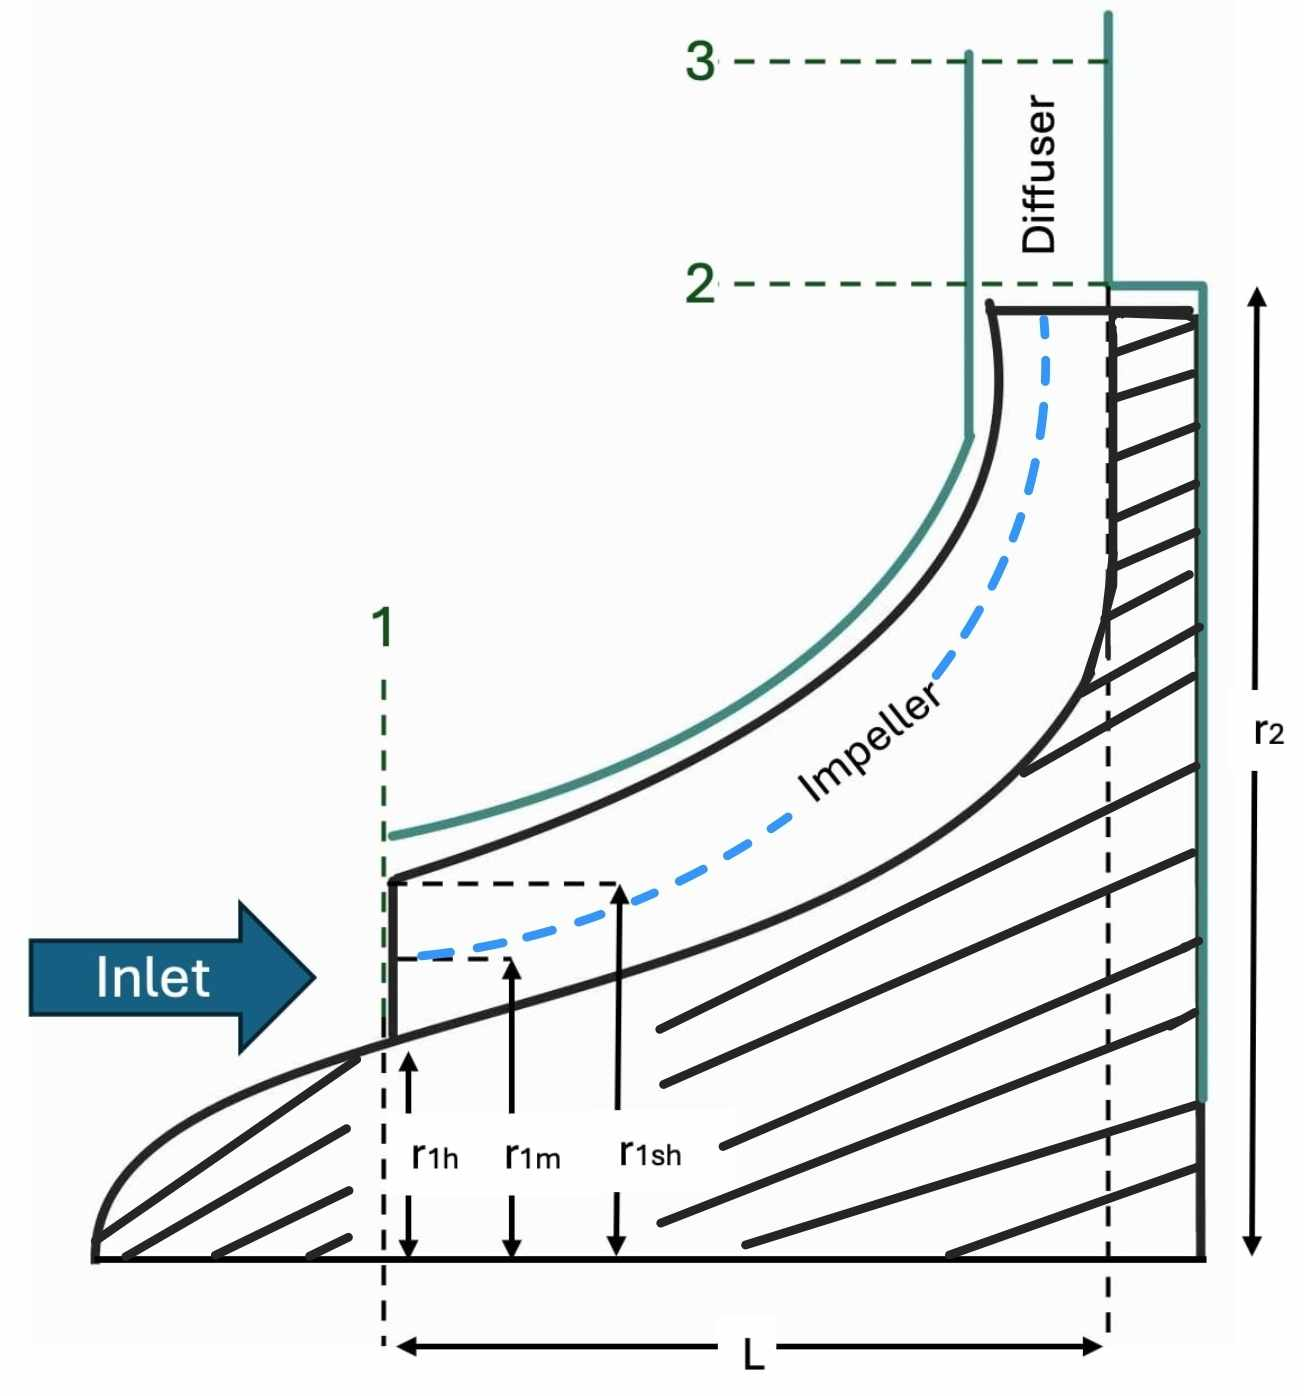
\includegraphics[width=0.5\textwidth]{figures/HPCdesign.jpeg}
    \caption{High Pressure Compressor Stages \cite{lectureslides}}
    \label{fig:HPCdesign}
\end{figure}

\section{Impeller Inlet Design Parameters for Geometry}

The rotational speed equations, presented in \autoref{Rotational Speed}, were derived from the velocity triangle depicted in \autoref{fig:ImpellerInletVelocityTriangle}. These equations underwent iterative adjustments of density to ensure alignment with the desired rotational speed of the HPT. A suitable value for the specific speed ($N_s$) was selected within the range of 55 to 85 to minimize losses effectively \cite{lectureslides}.

\begin{table}[H]
    \centering
    \caption{Rotational Speed  \cite{lectureslides}}
    \begin{tabular}{|l|c|c|c|} \hline 
          \textbf{Step} &\textbf{Variable}&  \textbf{Equation}& \textbf{Value}\\ \hline 
          0.01&Centrifugal Specific Speed&   $N_s$ was iterated& $76.23$\\ \hline 
          0.02&Density&  ${\rho_1}$ was iterated& $2.950 \frac{kg}{m^3}=0.08355 \frac{kg}{ft^3}$\\ \hline 
          0.03&Volume Flow&   $Q = \frac{m_{03}}{\rho_1}$& $62.44 \frac{ft^3}{s}$\\ \hline 
          0.04&Isentropic Enthalpy Rise&  $\Delta h_{0,\text{is}} = c_{\text{pa}} \cdot (T_{04} - T_{03})$ & $200.7 \frac{kJ}{kg}=86.29 \frac{Btu}{lb}$\\ \hline 
          0.05&Rotational Speed&  $N=\frac{{(N_s (778.26 \cdot \Delta h_{0,\text{is}}))^{3/4}}}{{\sqrt{Q}}}$& $N=40,245rpm ; w=4214 \frac{rad}{s}$\\ \hline
    \end{tabular}
    \label{Rotational Speed}
\end{table}

\begin{figure}[H]
    \centering
    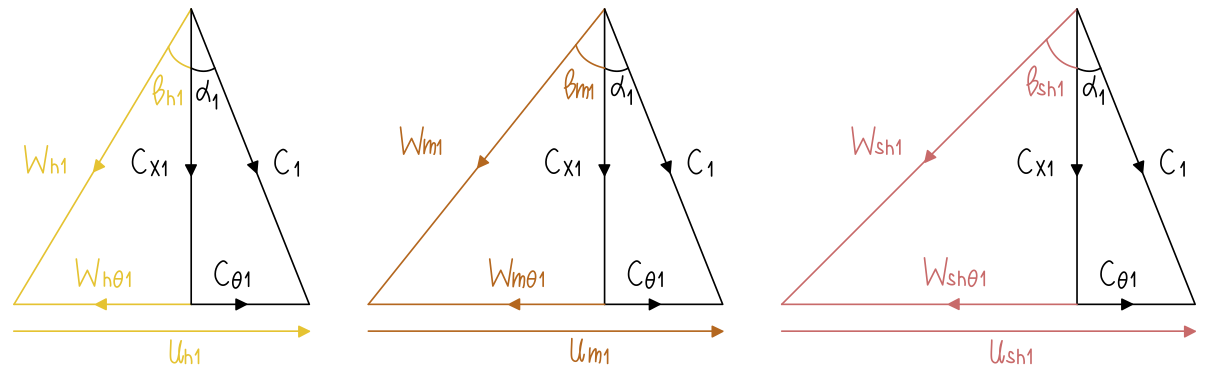
\includegraphics[width=1\textwidth]{figures/Impeller Inlet Velocity Triangle.png}
    \caption{Impeller Inlet Velocity Triangle \cite{lectureslides}}
    \label{fig:ImpellerInletVelocityTriangle}
\end{figure}

Similarly, the compressor's design formulas are outlined in \autoref{Compressor's Dimensions} and were derived from the principles illustrated in \autoref{fig:ImpellerExitVelocityTriangle} \cite{lectureslides}. Moreover, \autoref{fig:HPCdesign} provides examples of the radius configurations. Notably, there are fewer blades at the leading edge of the impeller compared to the trailing edge, owing to the presence of 16 splitter blades.

\begin{figure}[H]
    \centering
    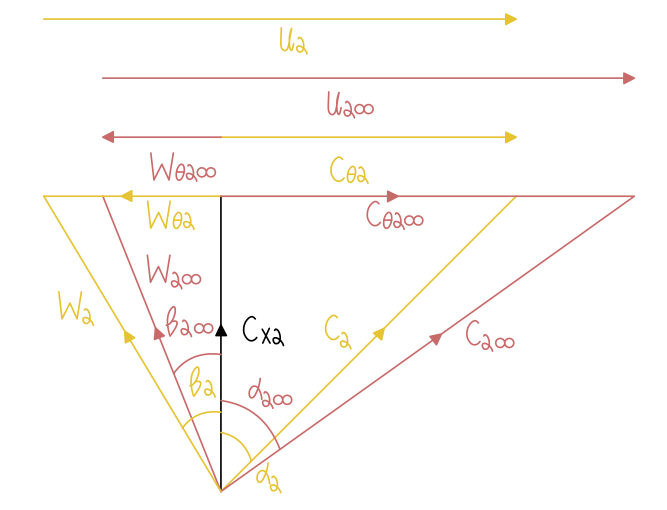
\includegraphics[width=0.5\textwidth]{figures/Impeller Exit Velocity Triangle.png}
    \caption{Impeller Exit Velocity Triangle \cite{lectureslides}}
    \label{fig:ImpellerExitVelocityTriangle}
\end{figure}

\begin{table}[H]
    \centering
    \caption{Compressor's Dimensions  \cite{lectureslides}}
    \begin{tabular}{|l|c|c|c|} \hline 
          \textbf{Step} &\textbf{Variable}&  \textbf{Equation}& \textbf{Value}\\ \hline 
         0.06&  Impeller Hub Leading Edge Radius&  $r_{1h}$ was iterated& $0.075m$\\ \hline 
         0.07&  Impeller Mean Leading Edge Radius&  $r_{1m}=\frac{r_{1h}+r_{1sh}}{2}$& $0.085m$\\ \hline 
         0.08&  Impeller Shroud Leading Edge Radius&  $r_{1sh}$ was iterated& $0.095m$\\ \hline 
         0.09&  Impeller Trailing Edge Radius&  $r_{2}$ was iterated& $0.125m$\\ \hline 
         0.10&  Radius Ratio&  $1.05\leq \frac{r_{3}}{r_{2}} \leq1.10$& $1.1$\\ \hline 
 0.11& Pressure Ratio& $0.9\leq\frac{r_{2}-r_{1h}}{L}\leq1.2$& $1.2$\\ \hline 
 0.12 & Diffuser Trailing Edge Radius & $r_{3}=r_{2} \cdot \frac{r_{3}}{r_{2}}$ & $0.1375m$\\ \hline 
0.13 & Compressor Length & $L=\frac{r_{2}-r_{1h}}{(\frac{r_{2}-r_{1h}}{L})}$& $0.04167m$\\ \hline 
0.14 & Etha max & $e_{max}$ was given& $0.01$\\ \hline 
0.15 & Impeller Exit Channel Height & $b_2= \frac{C_{r2} \cdot A_2}{C_2 \cdot2\pi \cdot r_2 (1-{B^*}_{2aero}-{B^*}_{2blade})}$& $0.00716m$\\ \hline 
0.16 & Trailing Edge Diffuser Height & $b_3=b_2$& $0.00716m$\\ \hline 
0.17 & Channel Height & $b_{2-3}=b_2$& $0.00716m$\\ \hline 
0.18 & Leading Edge Number of Blade & $N_{b1}$ was given& $16$\\ \hline 
0.19 & Trailing Edge Number of Blade & $N_{b2}$ was given& $32$\\ \hline
    \end{tabular}
    
    \label{Compressor's Dimensions}
\end{table}

\newpage

\autoref{tab:Incidence's Angles} shows the incidence's angles assumed for the compressor's design.

\begin{table}[H]
    \centering
    \caption{Incidence's Angles  \cite{lectureslides}}
    \begin{tabular}{|c|c|c|c|} \hline 
          \textbf{Step} &\textbf{Variable}&  \textbf{Equation}& \textbf{Value}\\ \hline 
         1.01&  Inlet Shroud Incidence's Angle&  $1\degree \leq i_{1sh} \leq 3\degree$& $2\degree$\\ \hline 
         1.02& Inlet Mean Incidence's Angle&  $2\degree \leq i_{1m} \leq 5\degree$& $4\degree$\\ \hline 
         1.03& Inlet Hub Incidence's Angle&  $5\degree \leq i_{1h} \leq 9\degree$& $7\degree$\\ \hline
    \end{tabular}
    
    \label{tab:Incidence's Angles}
\end{table}

The formulas utilized to derive the parameters and values for the first stage are displayed in \autoref{Stage 1}. Iterating the inlet swirl angle is crucial to achieving a high level of efficiency. Furthermore, shock waves are not expected, it's crucial that all of the Mach numbers are less than 1.

\begin{table}
    \centering
    \caption{Stage 1  \cite{lectureslides}}
    \begin{tabular}{|l|c|c|c|} \hline 
          \textbf{Step} &\textbf{Variable}&  \textbf{Equation}& \textbf{Value}\\ \hline 
1.04&  Inlet Temperature&  $T_{01}=T_{03:Part A}$& $463.1K$\\ \hline 
1.05&  Mass Flow Rate&  $\dot m_1= \dot m_{02}$& $5.216 \frac{kg}{s}$\\ \hline 
1.06&  Eye Are&  $\pi ({r_{1sh}}^2 - {r_{1h}}^2)$& $0.011m^2$\\ \hline 
1.07&  Axial Velocity&  $C_{x1}=\frac{\dot m_1}{\rho \cdot A_{1sh}}$& $165.5 \frac{m}{s}$\\ \hline 
1.08&  Inlet Swirl&  $5\degree \leq \alpha_1 \leq 35\degree$ & $20 \degree = 0.3491 rad$\\ \hline 
1.09& Absolute Velocity& $C_1=\frac{C_{x1}}{cos(\alpha_1)}$& $176.1 \frac{m}{s}$\\ \hline 
1.10& Horizontal Absolute Velocity& $C_{\theta1}=\frac{C_{x1}}{tan(\alpha_1)}$& $60.24 \frac{m}{s}$\\ \hline 
1.11& Blade Velocity at Tip& $U_{1sh}=w \cdot r_{1sh}$& $400.4 \frac{m}{s}$\\ \hline 
1.12& Horizontal Relative Velocity at Tip& $W_{\theta1sh}=U_{1sh}-C_{\theta1}$& $340.1 \frac{m}{s}$\\ \hline 
1.13& Inlet Backsweep Angle at Tip& $\beta_{1sh}=tan^{-1}(\frac{W_{\theta1sh}}{C_{x1}})$& $1.118 rad = 64 \degree$\\ \hline 
1.14& Relative Velocity at Tip& $W_{1sh}=\sqrt{C_{x1}^2+W_{\theta1sh}^2}$& $378.3 \frac{m}{s}$\\ \hline 
1.15& Gas Constant& $R_{air}=\frac{(\gamma_a-1)c_{pa}}{\gamma_a}$& $0.2871 \frac{kJ}{mol \cdot K}$\\ \hline 
1.16& Relative Mach Number at Tip& $M_{rel.sh}=\frac{W_{1sh}}{\sqrt{\gamma_a \cdot R_{air} \cdot T_{01}}}$& $0.8767$\\ \hline 
1.17& Blade Velocity at Hub& $U_{1h}=r_{1h} \cdot w$& $316.1 \frac{m}{s}$\\ \hline 
1.18& Blade Velocity at Mean& $U_{1m}=r_{1m} \cdot w$& $358.2 \frac{m}{s}$\\ \hline 
1.19& Horizontal Relative Velocity at Hub& $W_{\theta1h}=U_{1h}-C_{\theta1}$& $255.8 \frac{m}{s}$\\ \hline 
1.20& Horizontal Relative Velocity at Mean& $W_{\theta1m}=U_{1m}-C_{\theta1}$& $298.0 \frac{m}{s}$\\ \hline 
1.21& Inlet Backsweep Angle at Hub& $\beta_{1h}=tan^{-1}(\frac{W_{\theta1h}}{C_{x1}})$& $0.9965rad=57 \degree$\\ \hline 
1.22& Inlet Backsweep Angle at Mean& $\beta_{1m}=tan^{-1}(\frac{W_{\theta1m}}{C_{x1}})$& $1.064rad=61 \degree$\\ \hline 
1.23& Relative Velocity at Hub& $W_{1h}=\sqrt{C_{x1}^2+W_{\theta1h}^2}$& $305 \frac{m}{s}$\\ \hline 
1.24& Relative Velocity at Mean& $W_{1m}=\sqrt{C_{x1}^2+W_{\theta1m}^2}$& $341 \frac{m}{s}$\\ \hline 
1.25& Relative Mach Number at Hub& $M_{rel.h}=\frac{W_{1h}}{\sqrt{\gamma_a \cdot R_{air} \cdot T_{01}}}$& $0.7063$\\ \hline 
1.26& Relative Mach Number at Mean& $M_{rel.m}=\frac{W_{1m}}{\sqrt{\gamma_a \cdot R_{air} \cdot T_{01}}}$& $0.7900$\\ \hline
1.27& Mean Metal's Angle& $\beta^*_{1m}=\beta_{1m}-i_{1m}$& $62 \degree$\\ \hline 
1.28& Shroud Metal's Angle& $\beta^*_{1sh}=\beta_{1sh}-i_{1sh}$& $57 \degree$\\ \hline 
1.29& Hub Metal's Angle& $\beta^*_{1h}=\beta_{1h}-i_{1h}$& $50 \degree$\\ \hline 
    \end{tabular}
    
    \label{Stage 1}
\end{table}

\section{Impeller Exit Design Parameters for Geometry}
%slip factor, velocity triangles, etc

The plots to get the $U_2$ corrected at various values of $B^*_2$ are \autoref{fig:U2 Correcte B=0}, \autoref{fig:U2 Correcte B=35}, and \autoref{fig:U2 Correcte B=45}. Furthermore, the exit design parameter values and equations are displayed in \autoref{tab:stage 2}. To get a good efficiency, the exit back sweep angle and the exit swirl angle were iterated values. In Step 2.14, the relative velocity ratio needed to be between 0.5 and 0.6 in order to avoid an overly aggressive design. As well as that, for the design to be considered, the meridional velocity ratio needed to fall between 0.8 and 1.0. Lastly, there needs to be convergence between the start and exit back sweep angle verifications. \par

\begin{figure}[H]
  \centering
  \begin{subfigure}{0.49\linewidth}
    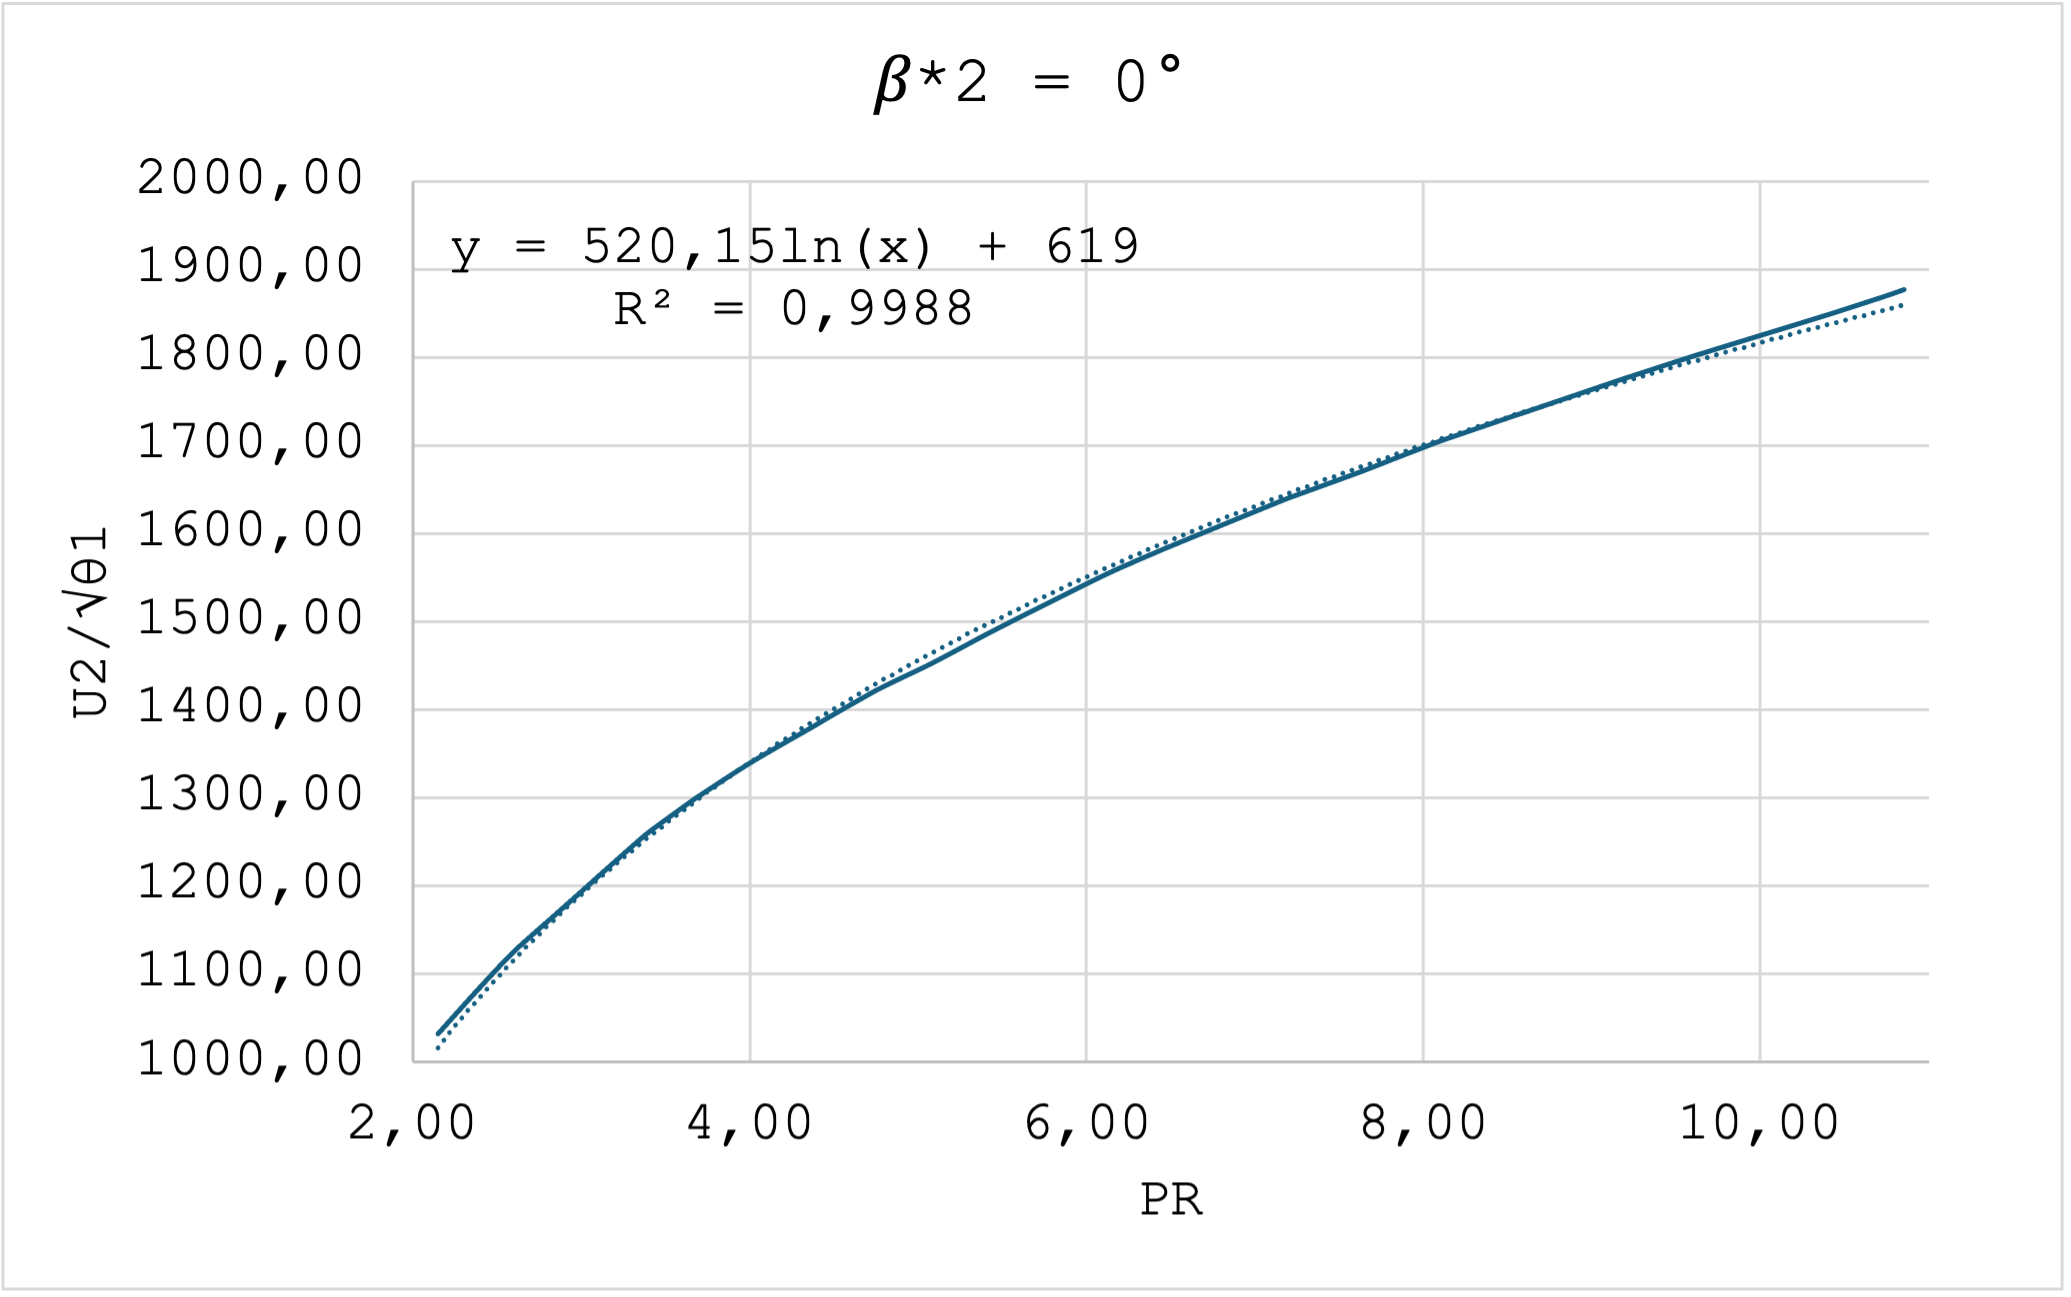
\includegraphics[width=\linewidth]{figures/B2=0.png}
    \caption{$U_2 \hspace{0.15cm} Corrected \hspace{0.15cm} for \hspace{0.15cm} \beta_2^*=0\degree$ \cite{lectureslides}}
    \label{fig:U2 Correcte B=0}
  \end{subfigure}
  \hfill
  \begin{subfigure}{0.49\linewidth}
    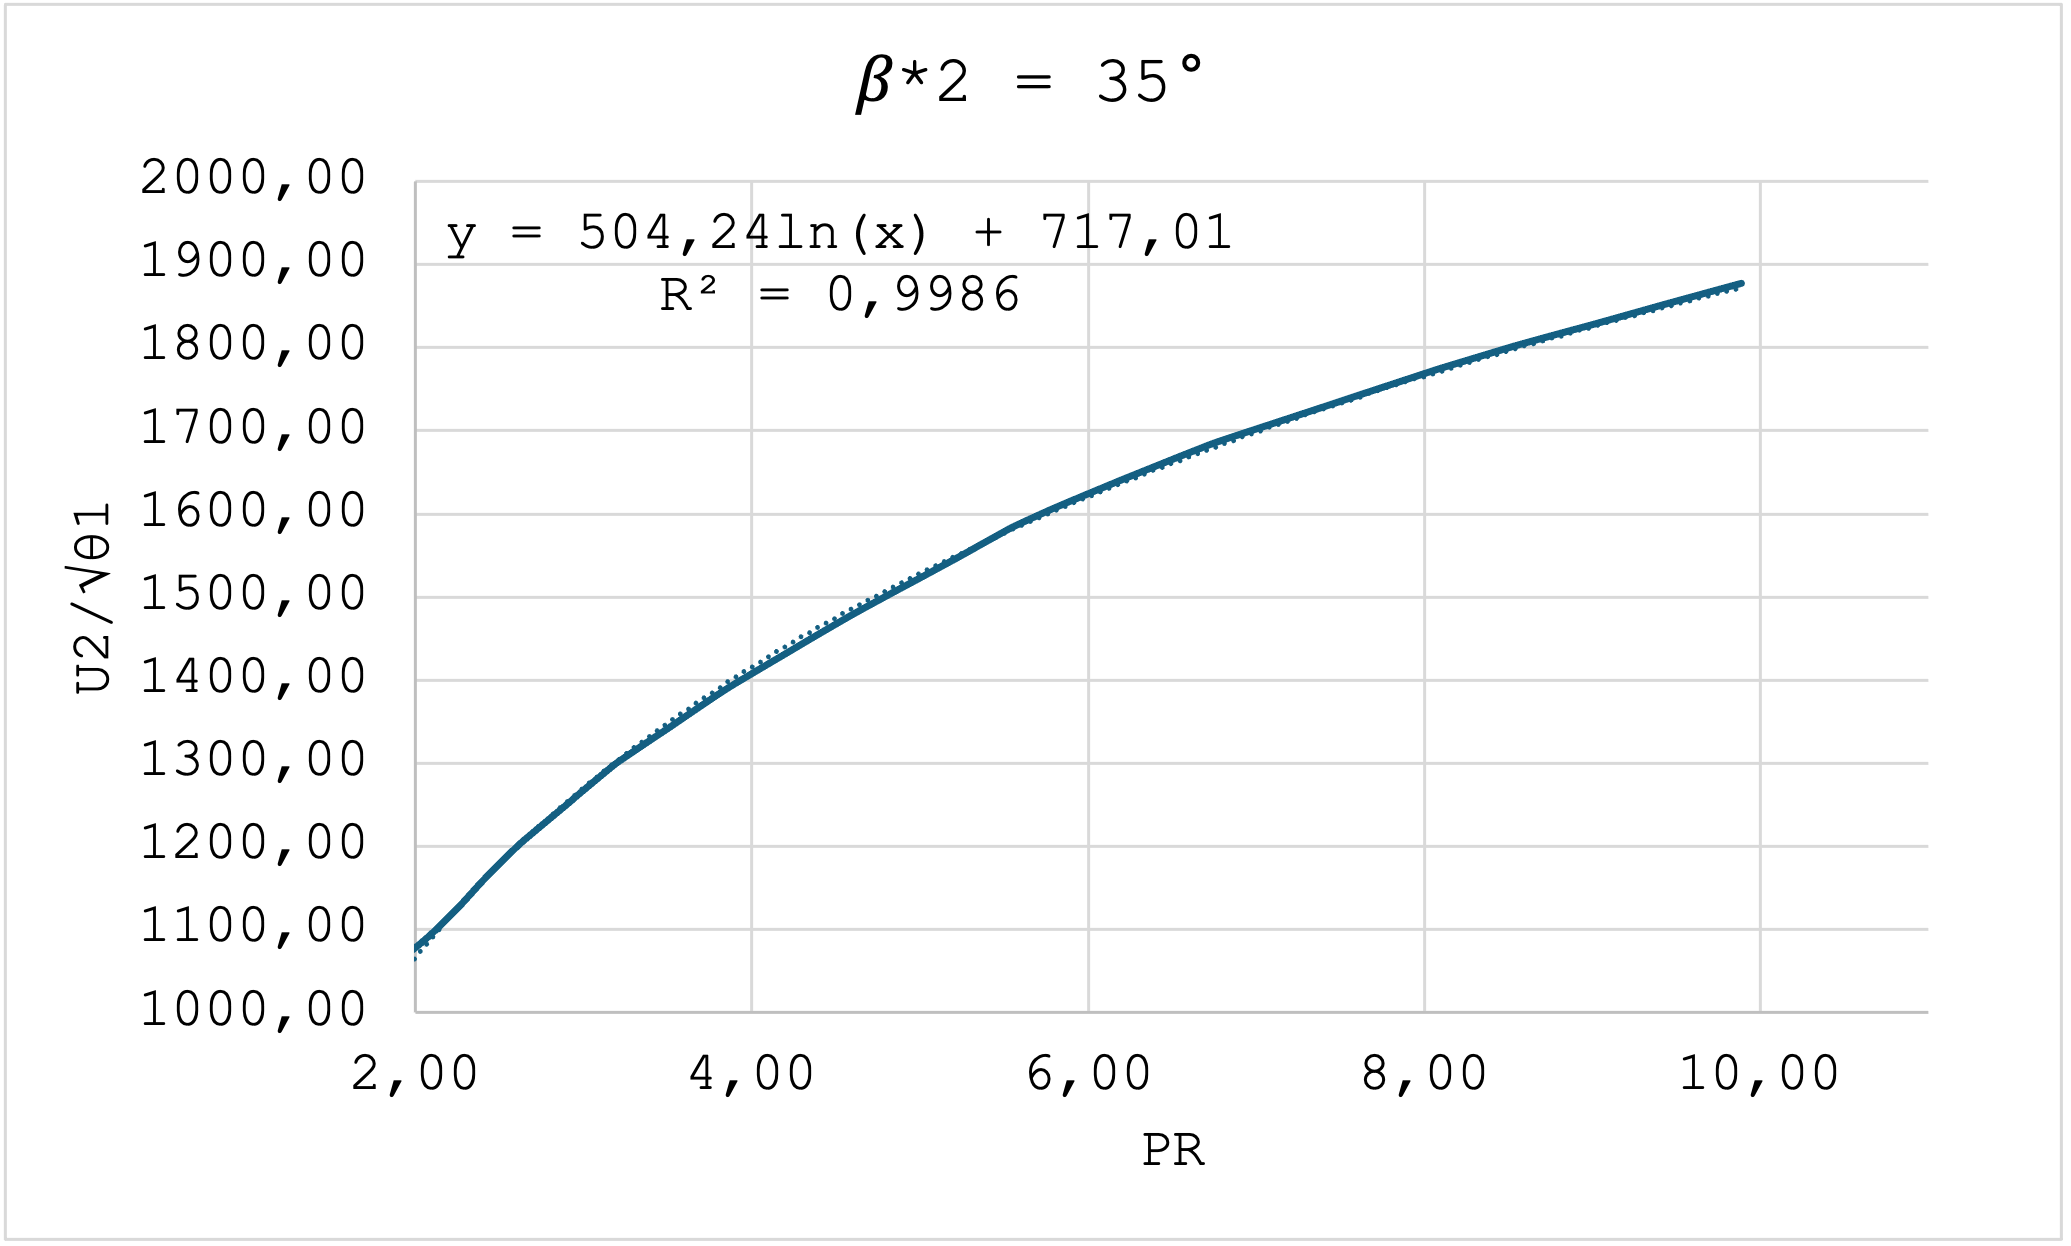
\includegraphics[width=\linewidth]{figures/B2_35.png}
    \caption{$U_2 \hspace{0.15cm} Corrected \hspace{0.15cm} for \hspace{0.15cm} \beta_2^*=35\degree$ \cite{lectureslides}}
    \label{fig:U2 Correcte B=35}
  \end{subfigure}
  
  \vspace{20pt}
  
  \begin{subfigure}{0.49\linewidth}
    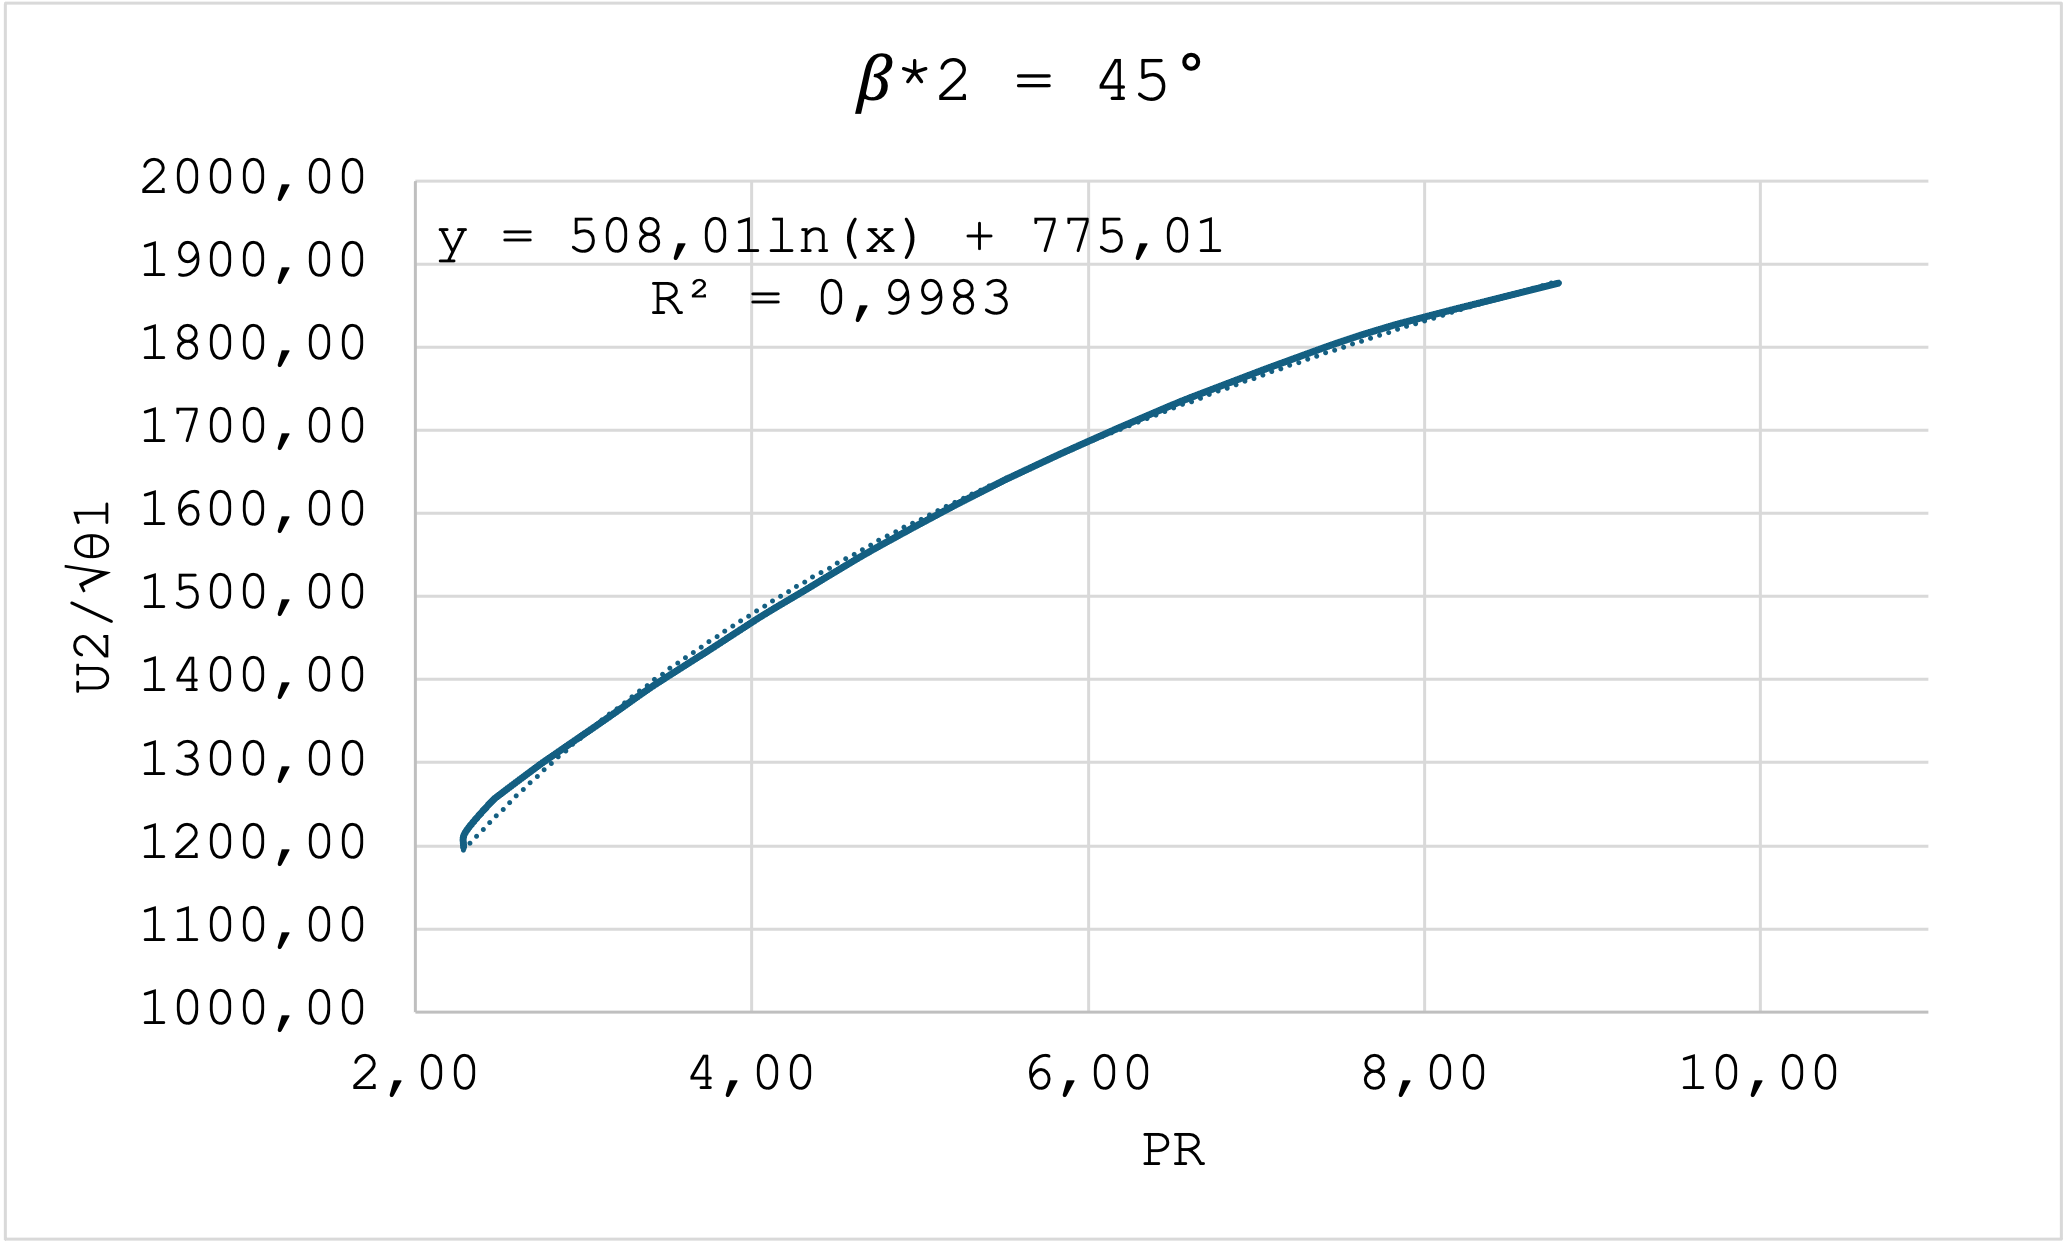
\includegraphics[width=\linewidth]{figures/B2=45.png}
    \caption{$U_2 \hspace{0.15cm} Corrected \hspace{0.15cm} for \hspace{0.15cm} \beta_2^*=45\degree$ \cite{lectureslides}}
    \label{fig:U2 Correcte B=45}
  \end{subfigure}
  \hfill

  \caption{Blade Velocity Corrected for Differing $\beta_{2}^{\star}$ Angles}
  \label{fig:Blade Velocity Corrected for Differing  Angles}
\end{figure}

\begin{table}[H]
    \centering
    \caption{Stage 2  \cite{lectureslides}}
    \begin{tabular}{|l|c|c|c|} \hline 
          \textbf{Step} &\textbf{Variable}&  \textbf{Equation}& \textbf{Value}\\ \hline 
         2.01&  Exit Backsweep Angle&  $0\degree \leq {\beta^*}_2 \leq 40\degree$& $31 \degree=0.5411rad$\\ \hline 
         2.02&  Flow Turning Angle&  $\theta_1=\frac{T_{01} \cdot 1.8}{518.7}$& $1.607$\\ \hline 
         2.03&  Speed Ratio&  \autoref{fig:U2 Correcte B=35}& $1262 \frac{ft}{s}$\\ \hline 
         2.04&  Impeller Exit Speed&  $U_2=(\frac{U_2}{\sqrt{\theta_1}}) \cdot \sqrt{\theta_1}$& $1599 \frac{ft}{s}= 487.5 \frac{m}{s}$\\ \hline 
         2.05&  Outlet Temperature&  $T_{02}=T_{03.partA}$& $662.8K$\\ \hline 
         2.06&  Enthalpy's Change&  $\Delta h_0=c_{pa} \cdot (T_{02}-T_{01})$& $200.7 \frac{kJ}{kh}$\\ \hline 
         2.07&  Horizontal Absolute Velocity&  $C_{\theta2}=\frac{\delta h_0-C_{\theta1} \cdot U_{1m}}{U_2}$& $367.4 \frac{m}{s}$\\ \hline 
         2.08&  Exit Swirl&  $\beta_2>{\beta^*}_2$& $37 \degree=0.6458rad$\\ \hline 
         2.09&  Horizontal Relative Velocity&  $W_{\theta2}=U_2-C_{\theta2}$& $120.1 \frac{m}{s}$\\ \hline
 2.10& Axial Velocity& $C_{r2}=\frac{W_{\theta2}}{tan(\beta_2)}$& $159.4 \frac{m}{s}$\\\hline
 2.11& Relative Velocity& $W_2=\frac{W_{\theta2}}{tan(\beta_2)}$& $199.6 \frac{m}{s}$\\\hline
 2.12& Outlet Swirl& $\alpha_2=tan^{-1} (\frac{C_{\theta2}}{C_{r2}})$& $1.161rad=67 \degree$\\\hline
 2.13& Absolute Velocity& $C_2=\sqrt{C_{\theta2}^2+C_{r2}^2}$& $400.5 \frac{m}{s}$\\\hline
 2.14& Relative Velocity Ratio& $\frac{W_2}{W_{1sh}}$& $0.5276$\\\hline
 2.15& Meridional Velocity Ratio& $\frac{C_{r2}}{C_{x1}}$& $0.9629$\\\hline
 2.16& Thermo Work& $W_{thermo}=\frac{W_{HPC}}{5.216}$& $200.7 \frac{kJ}{kg}$\\\hline
 2.17& Slip Factor& $\sigma=1-\frac{0.63 \pi}{N_{b3}}$& $0.9381$\\\hline
 2.18& Exit Backsweep Angle VERIFICATION& ${\beta^*}_2=tan^{-1} (\frac{U_2-\frac{C_{\theta2}}{\sigma}}{C_{r2}})$& $0.5416rad=31\degree$\\\hline
 2.19& Mass Flow Rate& $\dot m_2= \dot m_1$& $5.216 \frac{kg}{s}$\\\hline
 2.20& Impeller Outlet Area& $A_2=\frac{A_{1sh} \cdot C_{x1}}{C_{r2}}$& $0.01109m^2$\\\hline
 2.21& B*aero& $0.12 \leq B^*_{2(aero)} \leq 0.17$& $0.17$\\\hline
 2.22& B*blade& $0.03 \leq B^*_{2(blade)} \leq 0.06$& $0.05$\\\hline
 2.23& B*2& $B^*_2=B^*_{2(aero)}+B^*_{2(blade)}$& $0.2150$\\\hline
 2.24& Density& $\rho_2=\frac{\dot m_2}{A_2 \cdot C_{r2}}$& $2.950\frac{kg}{m^3}$\\\hline
    \end{tabular}
    
    \label{tab:stage 2}
\end{table}

As depicted in \autoref{fig:VanelessDiffuserStability}, the flow passing through the vaneless diffuser exhibits distinct stable and stalling regions, delineated by a blue curve. Designs positioned above this curve are considered stable. Our design, as shown in \autoref{fig:VanelessDiffuserStability}, resides comfortably within the stable region. Therefore, the assumptions guiding its development were deemed valid.

\begin{figure}[H]
    \centering
    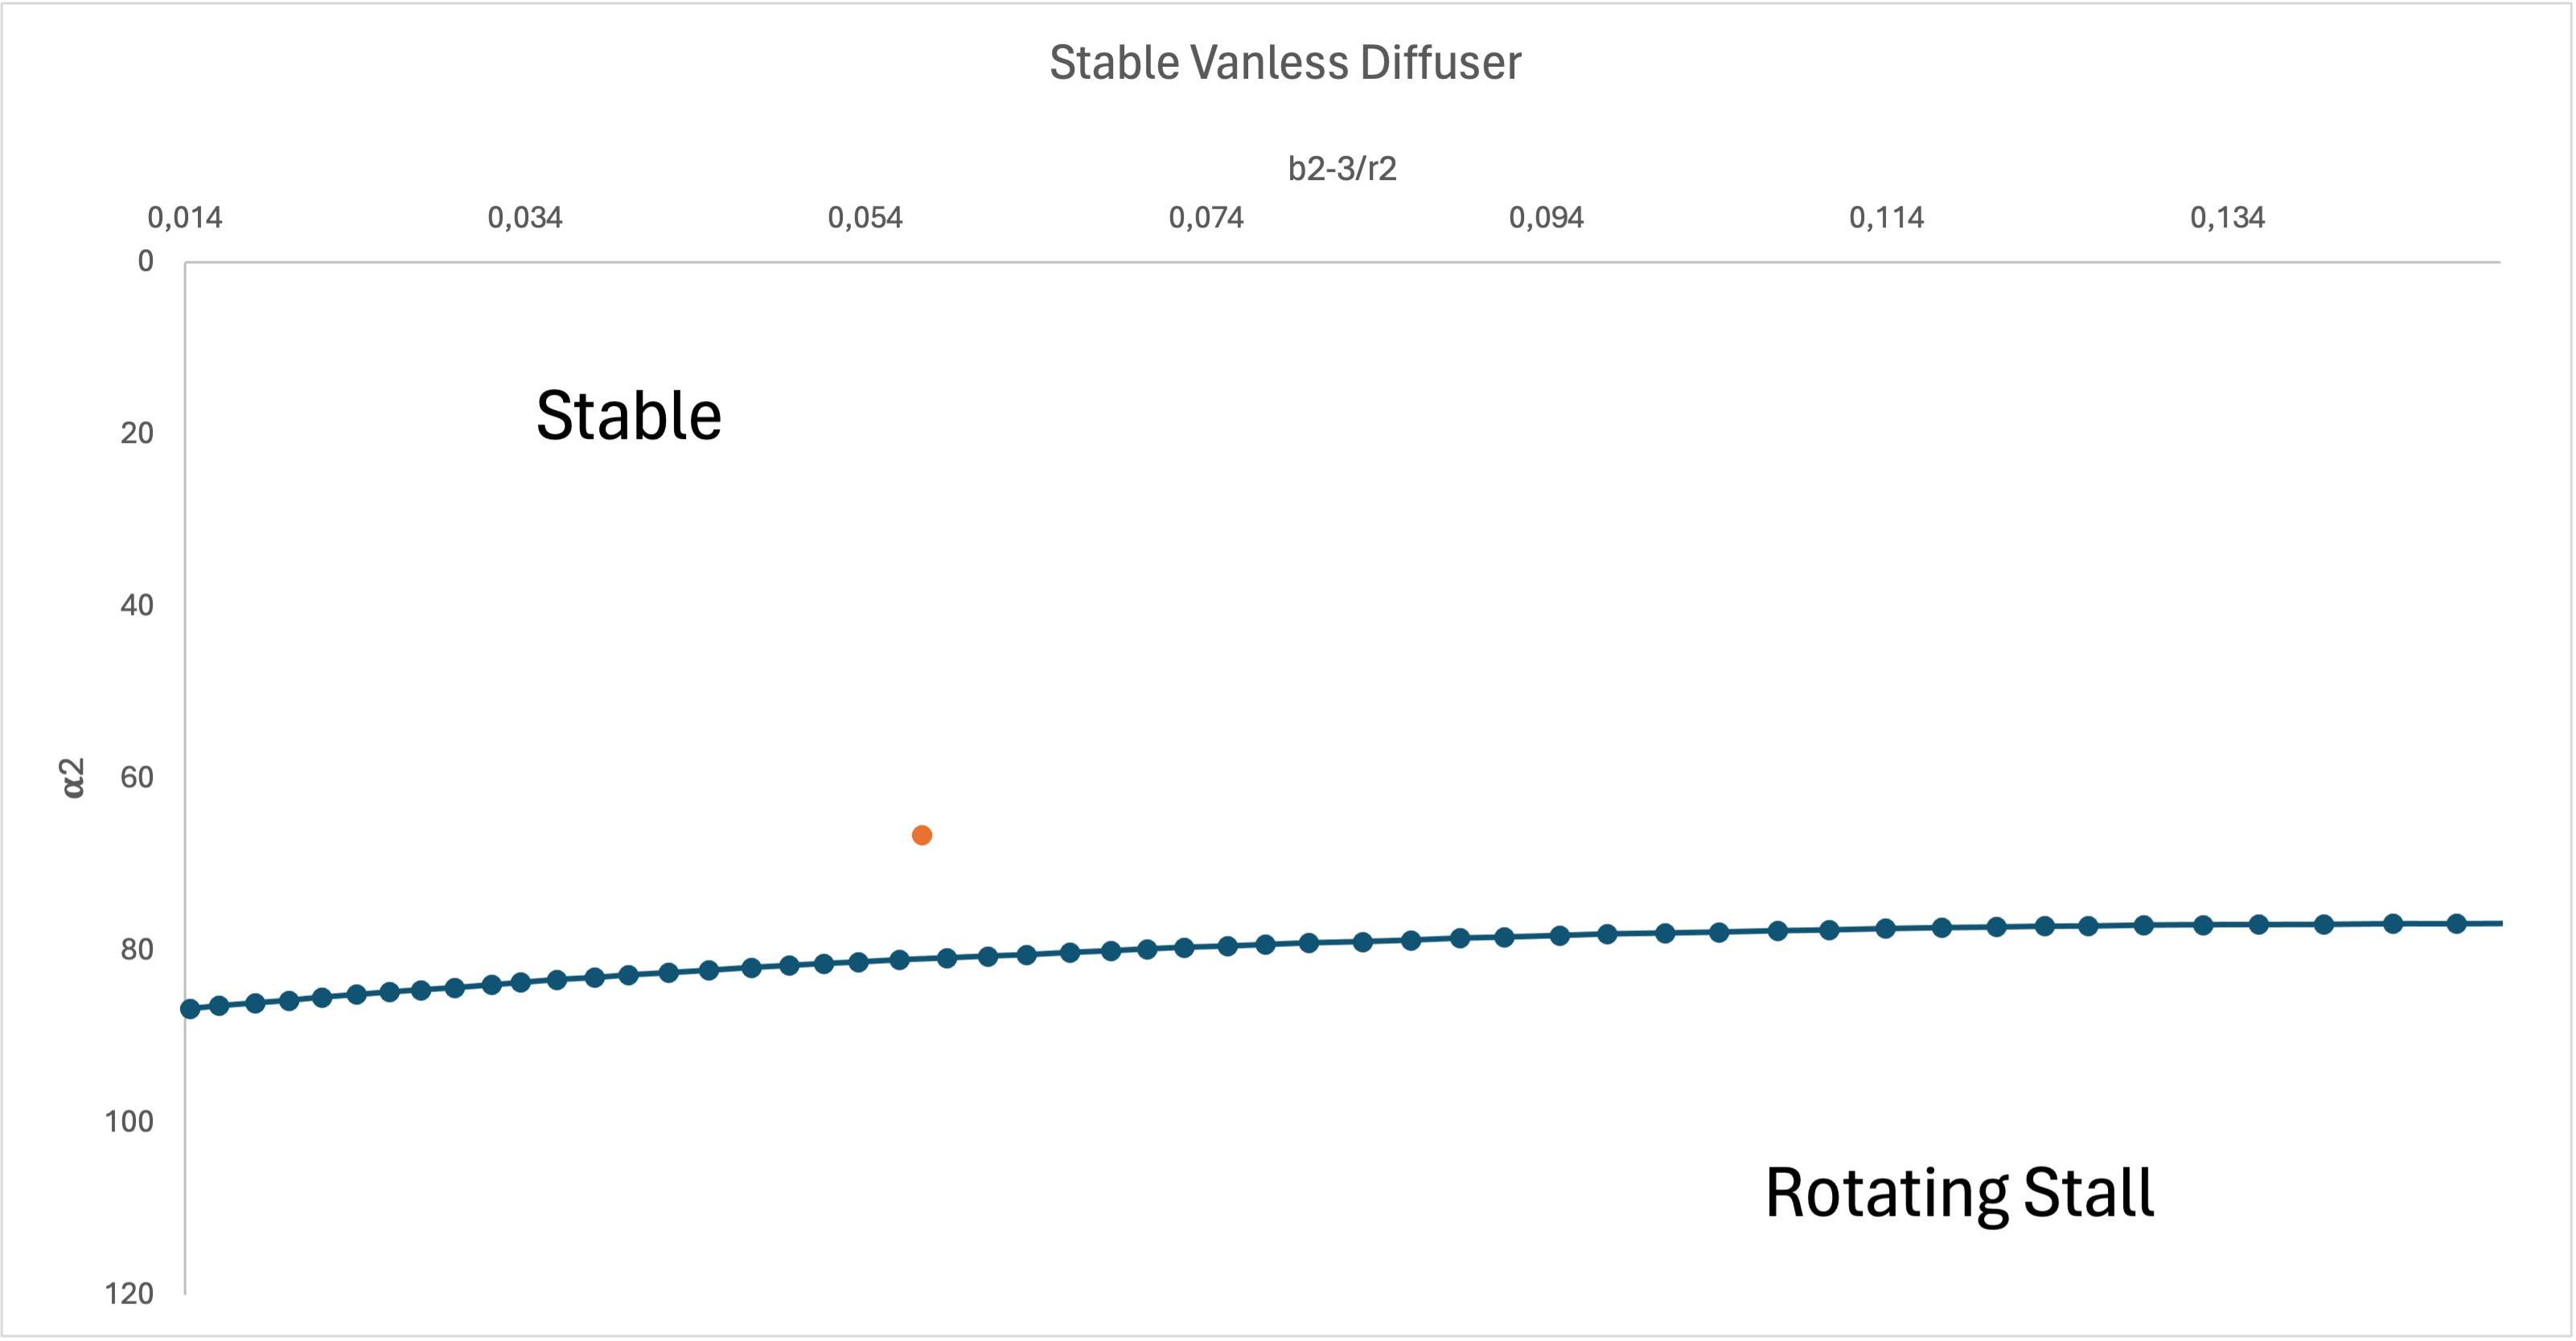
\includegraphics[width=1\textwidth]{figures/StableVanlessDiffuser.png}
    \caption{Vaneless Diffuser Stability \cite{lectureslides}}
    \label{fig:VanelessDiffuserStability}
\end{figure}

\section{Diffuser Design Parameters}
The diffuser exit's design parameter values and equations are displayed in \autoref{tab:stage 3}. The density was an important parameter to iterate in order to obtain accurate results at the throat. Finally, the throat aspect ratio is within the range of 0.8 and 1.2.


\begin{table}[H]
    \centering
\caption{Stage 3  \cite{lectureslides}}
\label{tab:stage 3}
    \begin{tabular}{|c|c|c|c|} \hline 
        \textbf{Step} &\textbf{Variable}&  \textbf{Equation}& \textbf{Value}\\ \hline  
         3.01&  Inlet Impeller Pressure&  $P_{01} = P_{02:Part A}$& 401.2 kPa\\ \hline 
         3.02&  Adiabatic Efficiency&  $\eta$ was given& 0.8850\\ \hline 
         3.03&  Outlet Impeller Pressure&  $P_{02} = P_{01}\left(\frac{\eta}{T_{01}} \left(T_{02} - T_{01}\right) + 1 \right)^{\frac{\gamma_{a}}{\gamma_{a} - 1}}$& 1244 kPa\\ \hline 
         3.04&  Vaneless Diffuser Exit Pressure&  $P_{03} = 0.99 * P_{02}$& 1232 kPa\\ \hline 
         3.05&  Horizontal Absolute Velocity&  $C_{\theta3} = C_{\theta2} \frac{r_{2}}{r_{3}} $& 334.0 $\frac{m}{s}$\\ \hline 
         3.06&  Diffuser Exit Area&  $ A_{3} = 2 \pi r_{3} b_{3} $& 6.186E-03 $m^{2}$\\ \hline 
         3.07&  Density&  $\rho_{3}$ was iterated& 3.089 $\frac{kg}{m^{3}}$\\ \hline 
         3.08&  Axial Velocity& $C_{r3} = C_2 * \left(\frac{r_2 * \rho_{2}}{r_3 * \rho_{3}} \right)$&  347.8  $\frac{m}{s}$\\ \hline 
         3.09&  Outlet Swirl&  $\alpha_{3} = tan^{-1}\left(\frac{C_{r3}}{C_{\theta3
         }}\right)$& 0.8055 rad  $(46.15\degree)$\\ \hline
 3.10& Absolute Velocity& $C_{3} = \sqrt{C_{r3}^{2} + C_{\theta3}^{2}}$&482.2 $\frac{m}{s}$\\\hline
 3.11& Stagnation Outlet Temperature& $T_{03}=T_{03.partA}$&662.8 K\\\hline
 3.12& Outlet Mach number& $\sqrt{\frac{C_{3}^{2}}{T_{03}\left(\gamma_{a}R_{air} - \frac{1}{2}\left(\gamma_{a} - 1\right)\frac{C_{3}^2}{T_{03}}\right)}}$&1.028\\ \hline 
 3.13& Static Outlet Temperature& $T_{3} = T_{03} - \frac{C_{r3}^{2}}{2c_{pa}}$&602.6 K\\\hline
 3.14& Static Pressure& $P_{3} = P_{03}\left(\frac{T_{03}}{T_{3}}\right)^{\frac{\gamma_{a} - 1}{\gamma_{a}}}$&1265.5 kPa\\\hline
 3.15& Density VERIFICATION& $\rho_{3} = \frac{\rho_{1}\left(\left(\gamma_{a} + 1\right)M_{3}^{2}\right)}{\left(\gamma_{a} - 1\right)M_{3}^{2} + 2}$&3.090 $\frac{kg}{m^{3}}$\\\hline
 3.16& Throat Blockage& B* was assumed&2.000E-02\\\hline
 3.17& Diameter& $d_{3} = 2r_{3}$&0.2750 m\\\hline
 3.18& Flow Incidence Angle& $i_{3}$ is assumed&-0.05236 rad $(-3.000\degree)$\\\hline
 3.19& Inlet Vane Angle& $\alpha_{3}* = \alpha_{3} - i_{3}$&0.8579 rad $(49.15\degree)$\\\hline
 3.20& Diffuser Vane Count& $18 \leq N_{v} \leq 25$&18\\\hline
 3.21& Throat Temperature& $T_{0}^{*} = T_{03}$ & 662.8 K \\\hline
 3.22& Throat Pressure& $P_{0}^{*} = P_{03}$ & 1231.6 kPa \\\hline
 3.23& Throat Mass Flow Rate& $\dot{m^{*}} = \rho^{*} * A_{3} * C_{r3} * 1.0125$ & 6.728 $\frac{kg}{s}$ \\\hline 
 3.24& Throat Mach Number& $M^{*}$ & 1.0 \\\hline
 3.25& Throat Area& $\frac{1}{A^{*}} = \frac{\sqrt{g\gamma_{a}}(1 - B^{*})P_{0}^{*}M^{*}}{\dot{m^{*}}\sqrt{R_{air}T_{0}^{*}}} (1+(\frac{\gamma_{a} - 1}{2}) M^{*2})^{\frac{-1 - \gamma_{a}}{2\gamma_{a} - 2}} $& 0.00113 $m^{2}$ \\\hline
 3.26& Individual Throat Area& $a^{*} = \frac{A^{*}}{N_v}$ & 0.00006299 $m^{2}$ \\\hline
 3.27& Diffuser Throat Width& $w^{*} = \frac{a^{*}}{b_3}$ & 0.0088 m \\ \hline 
 3.28& Throat Aspect Ratio& $AR_{th} = \frac{b^{*}}{w^{*}}$ & 0.8139 \\ \hline
    \end{tabular}
    
    
\end{table}

\clearpage
%%%%%%%%%%%%%%%%%%%%%%%%%%%%%%%%%%%%%%%%%%%%%%%%%%%%%%%%%%%%%%%%%%%%%%%%%%%%%%%%%%%%%%%%%%
%               PART C             %
%%%%%%%%%%%%%%%%%%%%%%%%%%%%%%%%%%%%%%%%%%%%%%%%%%%%%%%%%%%%%%%%%%%%%%%%%%%%%%%%%%%%%%%%%%
\chapter{High Pressure Turbine Design}

This section covers the aerodynamic design and performance analysis of the high pressure axial turbine. The methodology discussed in the following subsections is presented in the chronological order of the design. Section 2 concludes with an overview of how the high pressure turbine code is implemented in the Python programming language. 

\vspace{10pt}
\noindent \textbf{Note} that $\gamma$ is equal to 1.333, $c_{pg}$ is equal to 1.148 $kJ/{kg K}$ and R is equal to 0.287 $kJ/{kg K}$ in this section.\par





\section{High Pressure Turbine Design Approach}

An iterative approach has been used during the preliminary design phase of the high pressure turbine. \autoref{fig:xdsm_gt_design} presents a systematic approach taken by the turbine team to converge to a feasible design. The figure presents different systems used to navigate the feasible design space. \par 


Several constraints have been strictly implemented throughout the design process to contain the results in a finite and physically valid design space. These design constrants and checks have been discussed in detail in the following subsections. The design space is unimodel and hence, a global search strategy has been adopted for optimization \cite{mdobook}.
An XDSM diagram (\autoref{fig:xdsm_gt_design}) visually represents the interactions and data dependencies between different components, aiding in understanding the complex system \cite{mdobook}. 

\begin{figure}
    \centering
    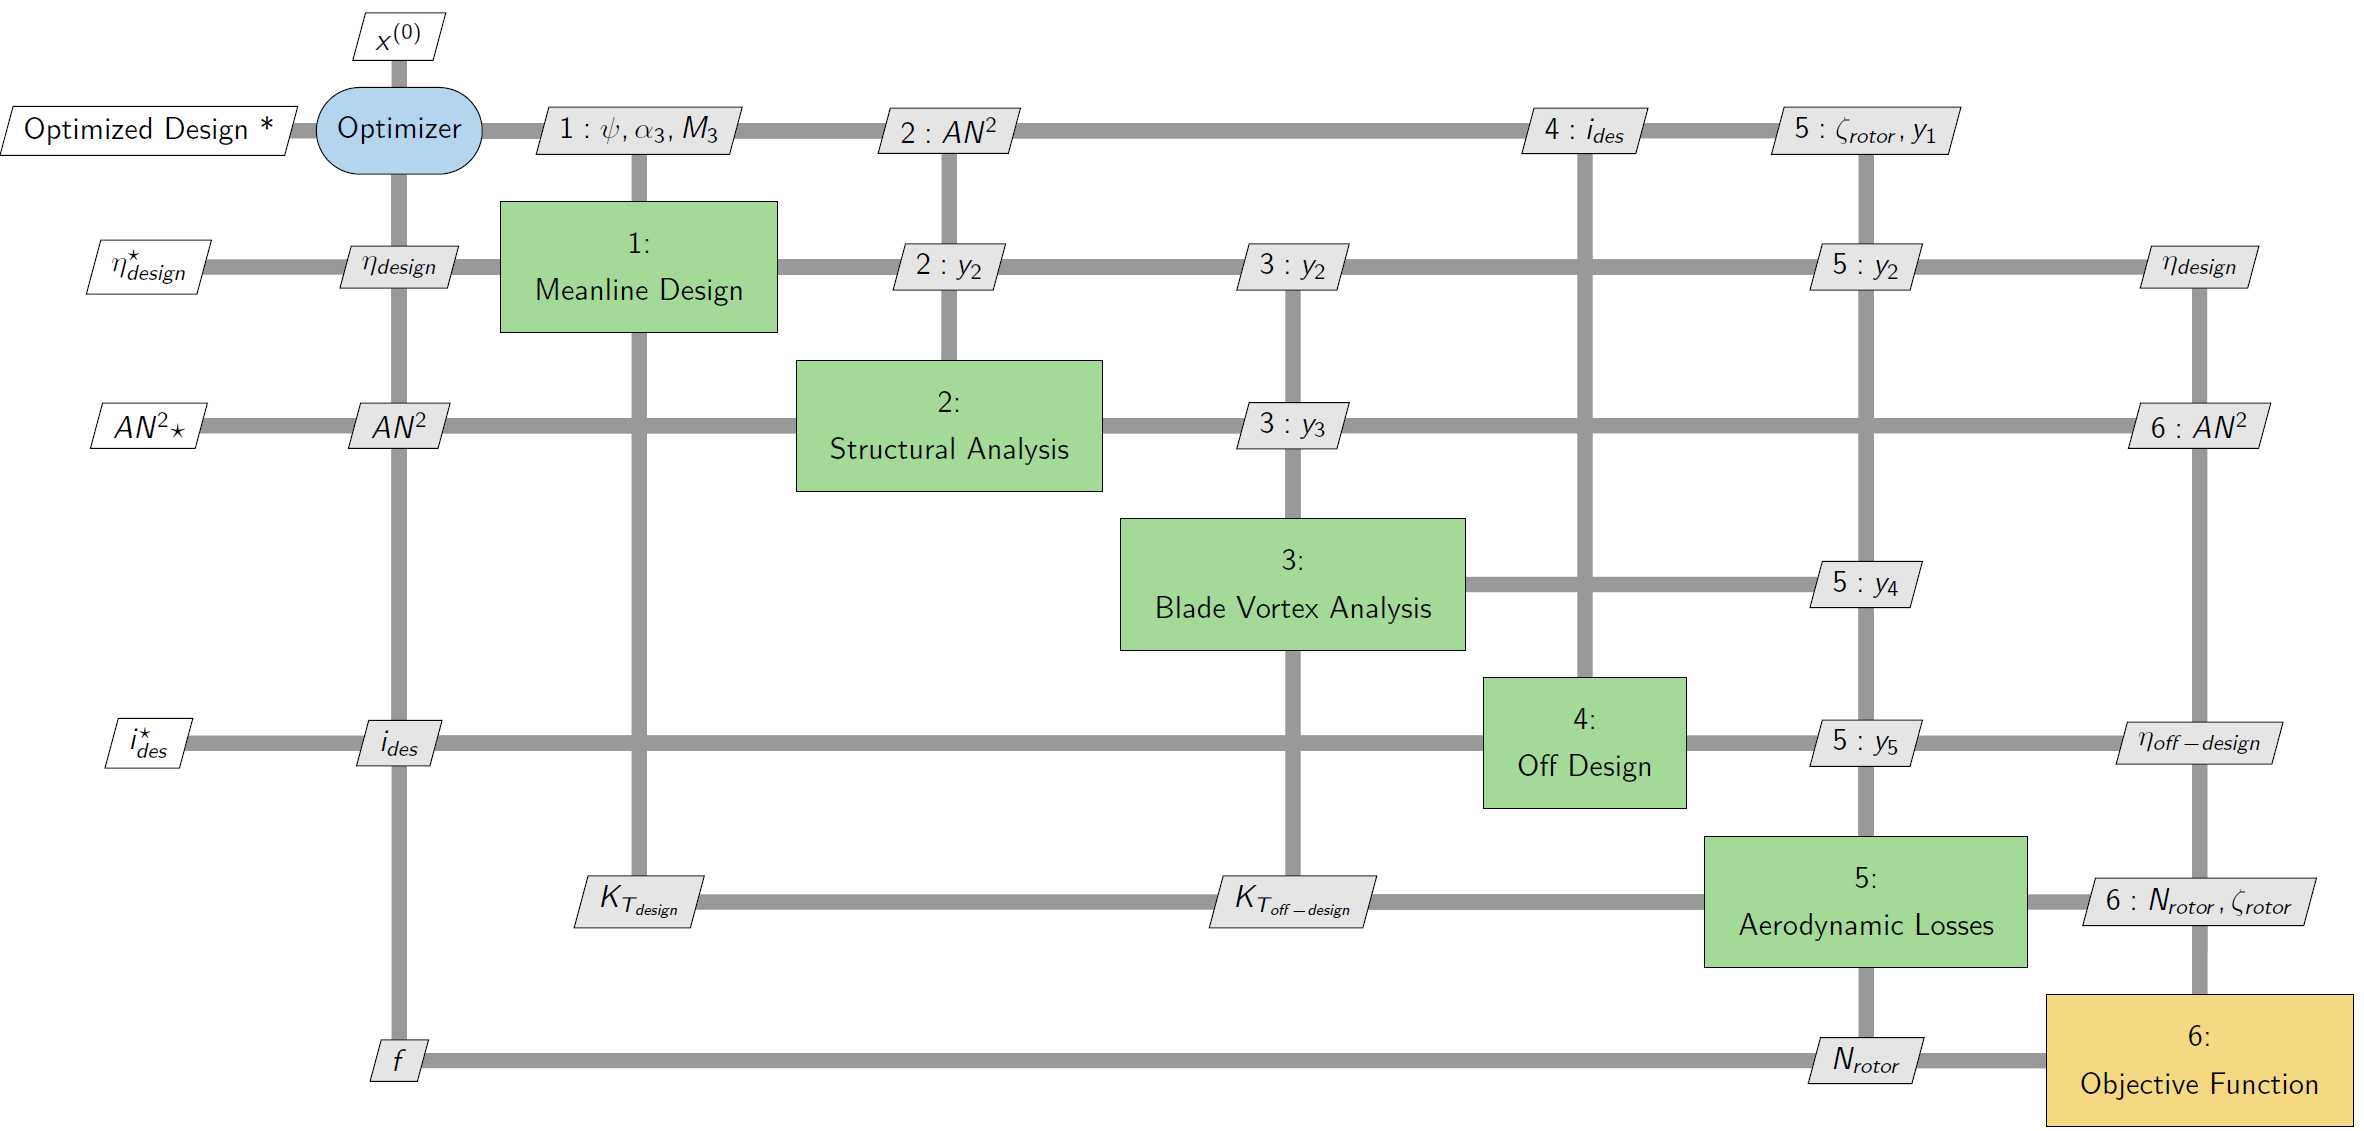
\includegraphics[width=0.99\linewidth]{figures/gt_xdsm.png}
    \caption{XDSM for High Pressure Turbine Design}
    \label{fig:xdsm_gt_design}
\end{figure}

The following procedure is used to formulate the optimization problem in order to derive at a design.
\begin{enumerate}
    \item Defining design variables.
    \begin{itemize}
        \item Design Efficiency
        \item Off Design Efficiency
        \item Number of Rotors
        \item Blade life
    \end{itemize}

    \item The method of weighted sums is used to define the optimization objective function. The idea is to combine all of the objectives into one objective function using weighted sums. However, the data is needed to be normalized first, thisis done using the following relation:
    \begin{equation}
        X_{\text{normalized}} = \frac{X - X_{\text{minimum}}}{X_{\text{maximum}} - X_{\text{minimum}}}
    \end{equation}

    \item The optimization function looks as following. The method of weighted sums is used to obtain the result of the optimization function. The data is analyzed using a global search optimization strategy.
    \begin{equation}
        y = f(\eta_{\text{final}}, \; \eta_{\text{final off-design}}, \; N_{\text{rotor}}, \; AN^2)
    \end{equation}
    \begin{equation}
        y = A \left( \frac{1}{\eta_{\text{final}}} \right) + B(\eta_{\text{final}} - \eta_{\text{final off-design}}) + C(N_{\text{rotor}}) + D(AN^2)
    \end{equation}
    The objective function $y = f(x)$ is minimized to obtain the optimized based on the chosen weights. Where A, B, C and D are the weights that can be tuned to optimize the design.

\end{enumerate}
 


\section{Meanline Design}
The meanline design covered in this section is the final result of the optimization process discussed previously. Note that from this section onward, station ``1" (shown as a subscript 01 or 1) refers to the vane/nozzle inlet, while station ``2" (subscript 02 or 2) is the vane exit/rotor inlet and station ``3" (subscript 03 or 3) refers to the vane exit. Finally, angles denoted as $\alpha$ and $\beta$ refer to the absolute and relative flow angles, respectively (the angle nomenclature used is consistent with Saravanamuttoo)\par

The table below summarizes several key input parameters. The reaction is temperature-based, the stage loading follows the Saravanamuttoo definition (twice that of Moustapha) and the $\alpha_3$, mach at exit ($M_3$) and $AN^2$ are within the ranges specified in the problem statement - note that each of these factors are inputs to the design process and the final values shown in the table below are the result of the optimization process described in the previous subsection. The shaft speed is also within the acceptable range provided by the compressor group. The temperature-based reaction of 0.527 is slightly higher than some turbines (typically in the 0.45-0.49 range \cite{saravanamuttoo2017}) because in this particular design, there is vane cooling assumed to be directly on the vanes while only disc cooling on the rotor. It is assumed that biasing the turbine slightly is acceptable under these conditions. \par

\begin{table}[H]
\caption{Dimensionless Parameters and Process Inputs}
\centering
\begin{tabular}{|c|c|p{0.6\textwidth}|}
\hline
\textbf{Property} & \textbf{Value} & \textbf{Source/Details}\\ \hline
$R_{mean}$ & 0.527 & Temperature-based. Detailed in "Station 2" subsection below. \\ \hline
$\psi$ & 3.21 (or 1.605 Moustapha) & Within the standard range in both Moustapha and Saravanamuttoo. 3.21 selected on the basis of optimization, discussed later in this report. \\ \hline
$U_{mean}$ & 363.2 m/s & Computed directly from the stage loading using the work in Part A.\\ \hline
$AN^2$ & $1.819x10^7 m^{2}rpm^{2}$ & Within the limits provided in the outline (units converted from imperial to metric). Selected based on optimization\\ \hline
$\omega$ & 4214.5 rad/s & Within operating limits of the compressor. Selected based on optimization procedure. \\ \hline
\end{tabular}
\label{tab:my_label}
\end{table}
\par

The code example below shows how the stage loading is used to compute $U_{mean}$.
\begin{figure}[H]
    \begin{minted}[frame=lines, fontsize=\footnotesize,linenos]{python}
def calc_U(psi):
    """
    This function calculates the metal speed U.
    Input:  Stage loading coefficient "psi"
    Output: Returns the value of U
    """
    U = numpy.sqrt((2*c_p_gas*1000*(T_02_cycle - T_03)) / (psi))
    return U
    \end{minted}
    \caption{Code snippet for calculation $U_{meanline}$.}
    \label{fig:code_U_meanline}
\end{figure}

Furthermore, the implementation of the meanline design in Python uses multiple checks to ensure that the design is conforming to physics and is following good design practices \cite{farokhi2022}. The table below summarizes the key checks used throughout the meanline design process.\par

\begin{table}[H]
\caption{Physics and Design Checks}
\centering
\begin{tabular}{|c|p{0.6\textwidth}|}
\hline
\textbf{Property}  & \textbf{Details}\\ \hline
$V_3 > V_2$ &  Ensures that relative velocity increases across the rotor\\ \hline
$C_2 > C_1$ & Ensures the absolute velocity increases across the stator\\ \hline
$U_{hub} < 335.28 m/s$ & Ensures the limit of 1100 ft/s at hub is not exceeded \\ \hline
$\rho_1 > \rho_2 > \rho_3$ & Ensures that density decreases across the turbine \\ \hline
$P_{03,rel} < P_{02,rel}$ & Physics check ensuring that relative stagnation pressure decreases across the turbine \\ \hline
$M_{2,hub} < 1$ & Ensures the largest value of absolute speed is below Mach 1 \\ \hline
$M_{3,rel,tip} < 1$ & Ensures the largest value of relative speed is below Mach 1 \\ \hline
\end{tabular}
\label{tab:my_label}
\end{table}
\par

Finally, some additional key assumptions include:
\begin{itemize}
    \item  Increasing axial velocity across the turbine.
    \item  The stator area is a converging duct
    \item  The rotor area is constant ($A_2 = A_3$)
\end{itemize}

\subsection{Station 1 - Nozzle/Vane Inlet}
From cycle calculations and the given information in the problem statement, station 1 (vane inlet) is completely defined. The table below summarizes the key properties of station 1. The third column shows the source of the information (either ``Cycle Calculations" from Part A, ``Given in Problem Statement" or ``Calculated") and detailed calculations follow the table for properties denoted as "Calculated". \par

\begin{table}[H]
\caption{Station 1 - Vane/Nozzle Inlet}
\centering
\begin{tabular}{|c|c|c|}
\hline
\textbf{Property} & \textbf{Value} & \textbf{Source}\\ \hline
$T_{01}$ & 1245.3 K & Cycle Calculations \\ \hline
$P_{01}$ & 1182.1 kPa & Cycle Calculations\\ \hline
$\dot{m}_1$ & 4.836 kg/s & Cycle Calculations\\ \hline
$T_{1}$ & 1242.1 K & Calculated \\ \hline
$P_{1}$ & 1169.8 kPa & Calculated\\ \hline
$\rho_{1}$ & 3.282 $kg/m^3$ & Calculated\\ \hline
$M_{1}$ & 0.125 & Given in Problem Statement\\ \hline
$C_1$ & 86.2 m/s & Calculated \\ \hline
$C_{w1}$ & 15 m/s & Calculated \\ \hline
$C_{a1}$ & 84.9 m/s& Calculated\\ \hline
$\alpha_1$ & -10 degrees & Given in Problem Statement\\ \hline
$A_1$ & 0.0174 & Calculated \\ \hline
\end{tabular}
\label{tab:my_label}
\end{table}


From the properties above, the meanline velocity triangle at station 1 is completed, as shown in the figure below (angles in degrees and velocities in m/s). 

\begin{figure}[H]
    \centering
    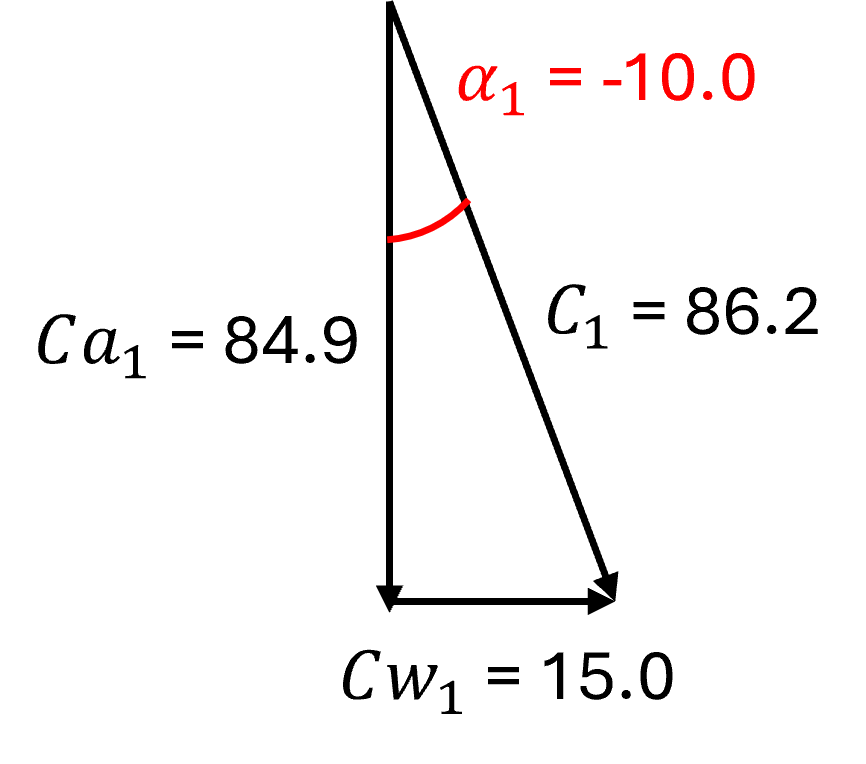
\includegraphics[width=0.3\linewidth]{figures/velocty_triangle_1.png}
    \caption{Velocity Triangle 1 - Nozzle Inlet}
    \label{fig:enter-label}
\end{figure}

\par
The code example below shows how the static temperature and pressure are obtained using the Mach number and the compressible flow equations. The static temperature is used to then compute the total speed ($C_1$), which with the given angle of $\alpha_1$ = -10, is used to obtain $C_{w1}$ and $C_{a1}$. 

\begin{figure}[H]
    \begin{minted}[frame=lines, fontsize=\footnotesize,linenos]{python}
def calc_properties(M, T_stagnation, P_stagnation):
    T = T_stagnation/(1 + ((gamma_g - 1)/2) * M**2)
    P = P_stagnation/((1 + ((gamma_g - 1)/2) * M**2))**(gamma_g/(gamma_g - 1))
    rho = P/(0.287*T)
    c = M * numpy.sqrt(gamma_g * 287 * T) 
    return T, P, rho, c
    \end{minted}
    \caption{Code snippet for calculating gas properties.}
    \label{fig:code_gas_properties}
\end{figure}
\par
The following subsection covers the mean line design at station 3 (rotor exit) which is necessary to complete before moving on to stage 2 (nozzle exit). 

\subsection{Station 3 - Rotor Exit}
The table below summarizes the gas properties at station 3 (rotor exit) in addition to key parameters such the velocities and angles. As in the previous subsection, the third column shows the source of the information. Detailed explanations follow the table for properties denoted as "Calculated". \par

\begin{table}[H]
\caption{Station 3 Properties - Rotor Exit}
\centering
\begin{tabular}{|c|c|p{0.6\textwidth}|}
\hline
\textbf{Property} & \textbf{Value} & \textbf{Source} \\ \hline
$T_{03}$ & 1041.3 K & Cycle Calculations\\ \hline
$P_{03}$ & 517.9 kPa & Cycle Calculations\\ \hline
$T_{3}$ & 996.4 K & Calculated - Same approach as station 1 in previous subsection\\ \hline
$P_{3}$ & 433.6 KPa & Calculated - Same approach as station 1 in previous subsection\\ \hline
$\rho_{3}$ & 1.53 $kg/m^3$ & Calculated - Same approach as station 1 in previous subsection\\ \hline
$\dot{m}_3$ & 5.06 kg/s & Cycle Calculations.\\ \hline
$C_3$ & 321.3 m/s & Calculated using Mach number and alpha 3 as inputs\\ \hline
$C_{a3}$ & 295.0 m/s & Calculated\\ \hline
$C_{w3}$ & 127.2 m/s & Calculated\\ \hline
$U_{mean}$ & 363.2 m/s & Calculated from Stage Loading \\ \hline
$\alpha_3$ & 23.3 degrees & Range Given in Problem Statement. Optimization process resulted in this value being selected.\\ \hline
$V_3$ & 572.3 m/s & Calculated \\ \hline
$V_{w3}$ & 490.5 m/s & Calculated\\ \hline
$\phi_3$ & 0.812 & Calculated\\ \hline
$\beta_3$ & 59.0 degrees & Calculated\\ \hline
$M_{3,rel}$ & 0.93 & Calculated\\ \hline
$P_{03,rel}$ & 743.3 kPa & Calculated\\ \hline
$A_3$ & 0.0123 $m^2$ & Calculated \\ \hline
\end{tabular}
\label{tab:my_label}
\end{table}
\par


From the properties above, the meanline velocity triangles at station 3 can be completed are and displayed in the figure below (angles in degrees and velocities in m/s).

\begin{figure}[H]
    \centering
    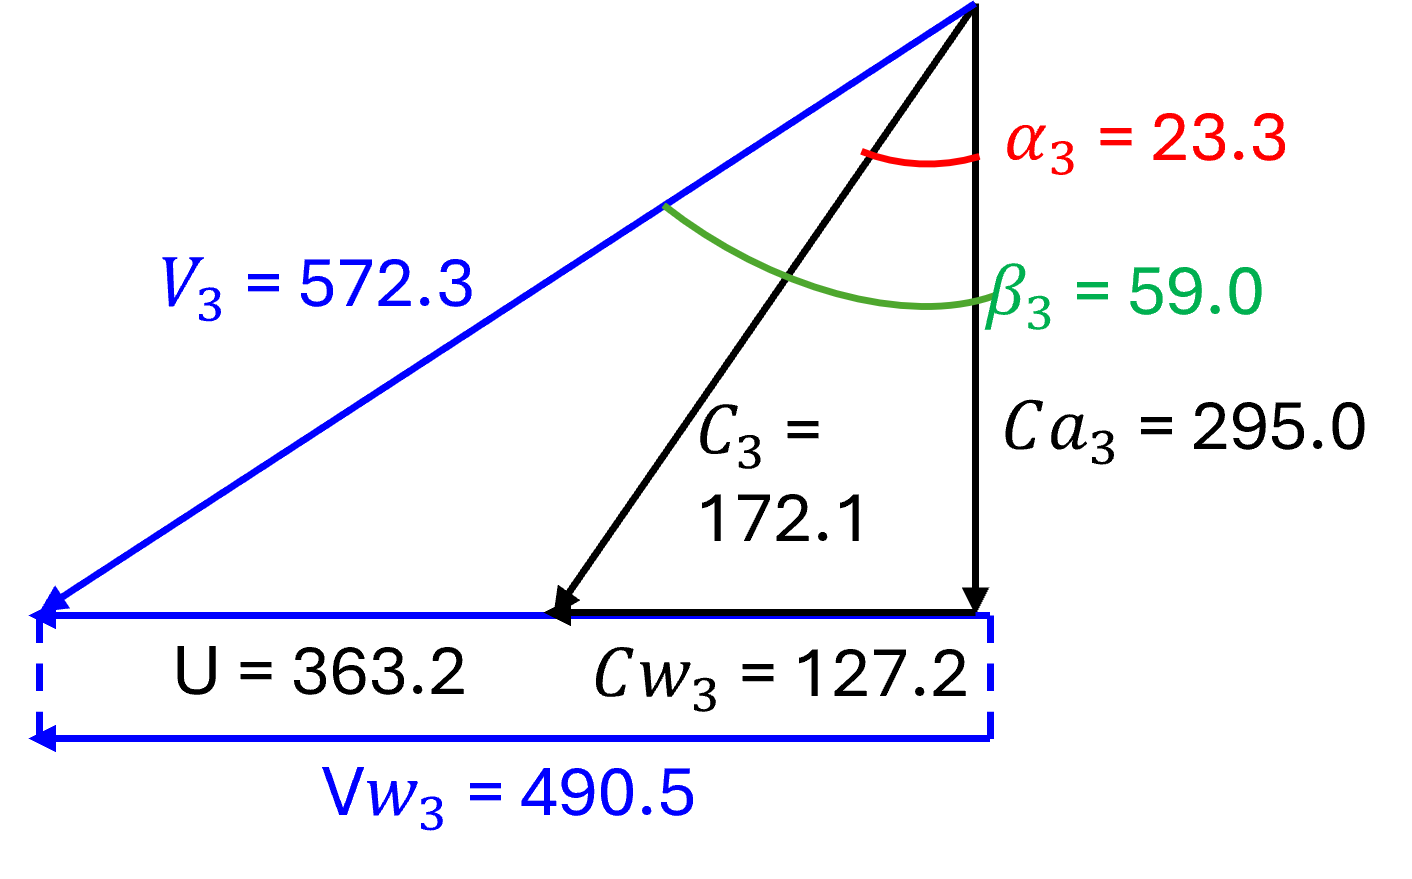
\includegraphics[width=0.4\linewidth]{figures/velocity_triangle_3.png}
    \caption{Velocity Triangle 3 - Rotor Exit}
    \label{fig:enter-label}
\end{figure}


Similar to previous subsection, all properties listed as "Calculated" are detailed below. Note that the gas properties ($\rho_3, P_3, T_3$) and total absolute velocity $C_3$ are calculated using the exact same process as outlined in the previous subsection for station 1. Based on the approach taken by the team, Mach number at the exit and absolute exit angle are inputs within the range provided in the outline.
\par


\begin{figure}[H]
    \begin{minted}[frame=lines, fontsize=\footnotesize,linenos]{python}
def calc_stage_3(U, C_3, T_3, rho_3,P_3,alpha_3):
    C_a_3 = C_3 * np.cos(np.radians(alpha_3))
    C_w_3 = math.sqrt(C_3**2 - C_a_3**2)
    V_w_3 = U + C_w_3
    alpha_3 = numpy.rad2deg(numpy.arcsin(C_w_3/C_3))
    V_3 = np.sqrt(V_w_3**2 + C_a_3**2)
    flow_coefficient_3 =  C_a_3 / U
    beta_3 = np.rad2deg(np.arctan(V_w_3 / C_a_3))
    a_3 = np.sqrt(gamma_g * R * 1000 * T_3)
    M_3_rel = V_3 / a_3
    A_3 = m_dot_3/(rho_3 * C_a_3)
    P_03_rel = P_3*(1+ (gamma_g-1)/2 * M_3_rel**2)**(gamma_g/(gamma_g-1))
    return C_a_3, C_w_3,  V_3, V_w_3, flow_coefficient_3, beta_3, a_3, M_3_rel, A_3, P_03_rel
    \end{minted}
    \caption{Code snippet for calculating properties for turbine stage 3.}
    \label{fig:code_stage_3}
\end{figure}

\par

\subsection{Station 2 - Nozzle Exit / Rotor Inlet}
With station 3 completed, station 2 can now be calculated. 
The table below summarizes the gas properties at station 2 (nozzle exit) in addition to the key parameters such as the temperature-based reaction, velocities and angles. 

\begin{table}[H]
\caption{Station 2 Properties - Nozzle Exit / Rotor Inlet}
\centering
\begin{tabular}{|l|c|c|}
\hline
\textbf{Property} & \textbf{Value} & \textbf{Source} \\ \hline
$T_{02}$ & 1225.9 K & Cycle Calculations\\ \hline
$P_{02}$ & 1182.2 kPa & Cycle Calculations\\ \hline
$T_{2}$ & 1122.3 K& Calculated\\ \hline
$P_{2}$ & 830.2 kPa & Calculated\\ \hline
$\rho_{2}$ & 2.577 $kg/m^3$ & Calculated\\ \hline
$\dot{m}_2$ & 4.98 kg/s & Cycle Calculations\\ \hline
$C_2$ & 487.9 m/s & Calculated\\ \hline
$C_{a2}$ & 172.1 m/s& Calculated\\ \hline
$C_{w2}$ & 456.5 m/s & Calculated\\ \hline
$U_{mean}$ & 363.2 m/s & Calculated \\ \hline
$\alpha_2$ & 69.3 degrees & Calculated\\ \hline
$V_2$ & 195.7 m/s & Calculated\\ \hline
$V_{w2}$ & 93.3 m/s & Calculated\\ \hline
$\phi_2$ & 0.4737 & Calculated\\ \hline
$\beta_2$ & 28.5 degrees & Calculated\\ \hline
$M_{2,abs}$ & 0.744 & Calculated \\ \hline
$P_{02,rel}$ & 880.7 kPa & Calculated\\ \hline
$A_2$ & 0.0123 $m^2$ & Equal to Area 3.\\ \hline
\end{tabular}
\label{tab:my_label}
\end{table}



From the properties in the table above, the velocity triangle in the image below is derived for station 2. The velocities are in units m/s and the angles in degrees. 

\begin{figure}[H]
    \centering
    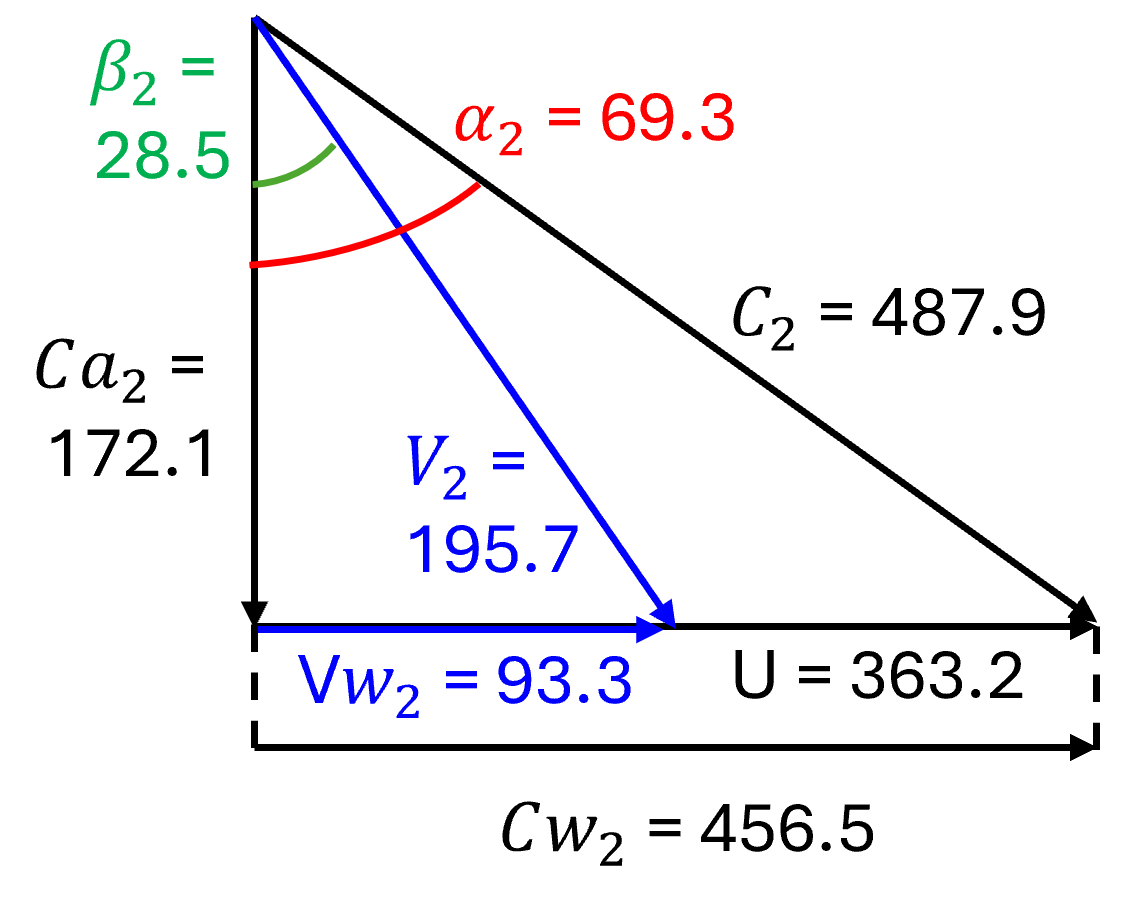
\includegraphics[width=0.4\linewidth]{figures/velocity_triangle_2.png}
    \caption{Velocity Triangle 2 - Rotor Inlet}
    \label{fig:enter-label}
\end{figure}

Similar to previous sections, all properties listed as ``Calculated" are detailed below. Note that this process requires iteration until convergence to ensure agreement between the equation of state (ideal gas law) and the conservation of mass. Also, $V_{w2}$ and $C_{w2}$, together with previously determined $V_{w3}$ and $C_{w3}$, ensure that the work always conforms to the turbine work needed in Part A. That is $Work = U_{mean} x (C_{w2} + C_{w3}) = U_{mean} x (V_{w2} + V_{w3})$ = 212 kJ/kg (as shown in Part A).Inputs that do not result in convergence are simply discarded and the next set of inputs is computed.

\par



\begin{figure}[H]
    \begin{minted}[frame=lines, fontsize=\footnotesize,linenos]{python}
def calc_stage_2_trial(U,T_1,T_3,P_3,A_3,V_w_3):
    error = 1
    max_iterations = 10000
    count = 0
    T_2 = 1060
    increment = 0.01
    V_w_2 = (c_p_gas * 1000 * (T_02_cycle - T_03) / (U)) - V_w_3
    C_w_2 = (V_w_2 + U)

    while count < max_iterations:
        
        P_2 = P_01 * ((T_2/T_02_cycle) ** (gamma_g/(gamma_g - 1))) 
        rho_2 = P_2/(R*T_2)
        T_02 = T_2 + (C_w_2**2 + (m_dot_2/(rho_2*A_3))**2)/(2*c_p_gas*1000)
        #print(T_02)
        error = np.abs(T_02_cycle - T_02) 
        count = count + 1
        if (0 < error < 0.001):
            break
        else:
            T_2 = T_2 + increment
    
    if count != max_iterations:
        reaction = (T_2 - T_3)/(T_1 - T_3)
        A_2 = A_3
        C_a_2 = (m_dot_2)/(rho_2 * A_2) 

        flow_coefficient_2 = C_a_2 / U
        a_2 = np.sqrt(gamma_g * R * 1000 * T_2)
        
        beta_2 = np.rad2deg(np.arctan(V_w_2 / C_a_2))
        V_2 = np.sqrt(V_w_2**2 + C_a_2**2)
        
        C_2 = np.sqrt(C_w_2**2 + C_a_2**2)
        alpha_2 = np.rad2deg(np.arctan(C_w_2/C_a_2))
        M_2 = C_2 / a_2
        M_2_rel = V_2 / a_2
        P_02 = P_2*(1+ (gamma_g-1)/2 * M_2**2)**(gamma_g/(gamma_g-1))
        P_02_rel = P_2*(1+ (gamma_g-1)/2 * M_2_rel**2)**(gamma_g/(gamma_g-1))

    return T_02, T_2, P_2, rho_2, A_2, C_a_2, flow_coefficient_2, a_2,
            V_w_2, beta_2, V_2, C_w_2, C_2, alpha_2, M_2, M_2_rel,P_02,P_02_rel, reaction

    \end{minted}
    \caption{Code snippet for calculating properties for turbine stage 3.}
    \label{fig:code_stage_2}
\end{figure}
% \cite{saravanamuttoo2017} <- This is the cohen textbook :)

\section{Free Vortex Design}
The free vortex design involves the calculation of the rotor hub and tip velocities and angles in addition to other parameters such as the blade height. It is assumed that the stagnation pressure and stagnation temperature are not a function of the radius, but that the static temperature and pressure do change with radius as the total speeds change radially. 

Before calculating the hub and tip velocities and angles, the rotational speed, hub radius, tip radius, meanline radius and blade height need to be computed. The table below shows the final values of these properties. 

\begin{table}[H]
\caption{Blade Dimensional Parameters and Shaft Speed}
\centering
\begin{tabular}{|l|c|c|}
\hline
\textbf{Property} & \textbf{Value} & \textbf{Source} \\ \hline
$\omega$ & 4214.5 rad/s & Calculated\\ \hline
$r_{hub}$ & 0.0758 m & Calculated\\ \hline
$r_{tip}$ &0.0966 m & Calculated\\ \hline
$r_{mean}$ &0.0862 m & Calculated\\ \hline
$h$ & 0.0207 m & Calculated \\\hline
\end{tabular} 
\label{tab:my_label}
\end{table}
\par

The calculations below show how the values in the table above were established. 

\begin{figure}[H]
    \begin{minted}[frame=lines, fontsize=\footnotesize,linenos]{python}
class aerostructural():
    def calc_structural(an_squared_pointer, area_2_pointer, U_meanline_pointer):
        N = numpy.sqrt((an_squared_pointer)/area_2_pointer)
        omega = N*2*numpy.pi/60
        r_meanline = U_meanline_pointer/omega
        h = (area_2_pointer * (N/60))/U_meanline_pointer
        r_hub = r_meanline - (h/2)
        r_tip = r_meanline + (h/2)
        return N, omega, r_hub, r_tip, r_meanline, h
    \end{minted}
    \caption{Code snippet for calculating shaft speed and radial dimensions.}
    \label{fig:code_structural}
\end{figure}





The hub triangles may now be computed based on the parameters above and the information from the preceding subsection. The table below shows the hub triangles, assuming a free vortex design.

\begin{table}[H]
\caption{Hub Properties}
\centering
\begin{tabular}{|l|c|c|}
\hline
\textbf{Property} & \textbf{Value} & \textbf{Source} \\ \hline
$T_{2,hub}$ & 1095.7 K & Calculated\\ \hline
$P_{2,hub}$ & 754.1 kPa & Calculated\\ \hline
$T_{3,hub}$ & 994.3 K & Calculated\\ \hline
$P_{3,hub}$ & 429.8 kPa & Calculated\\ \hline
$C_{2,hub}$ & 546.7 m/s & Calculated\\ \hline
$C_{a2}$ & 172.1 m/s & Calculated\\ \hline
$C_{w2,hub}$ & 520.4 m/s & Calculated\\ \hline
$U_{hub}$ & 319.5 m/s & Calculated\\ \hline
$C_{3,hub}$ & 328.5 m/s & Calculated\\ \hline
$C_{a3}$ & 295.0 m/s & Calculated\\ \hline
$C_{w3,hub}$ & 144.5 m/s & Calculated\\ \hline
$\alpha_{2,hub}$ & 71.7 degrees & Calculated\\ \hline
$\alpha_{3,hub}$ & 26.1 degrees & Calculated\\ \hline
$V_{2,hub}$ & 263.4 m/s  & Calculated\\ \hline
$V_{w2,hub}$ & 199.4 m/s& Calculated\\ \hline
$V_{3,hub}$ & 550.5 K & Calculated\\ \hline
$V_{w3,hub}$ & 464.8 m/s & Calculated\\ \hline
$\beta_{2,hub}$ & 49.2 degrees& Calculated\\ \hline
$\beta_{3,hub}$ & 57.6 degrees & Calculated\\ \hline
$M_{2,rel,hub}$ & 0.41 & Calculated\\ \hline
$M_{2,abs,hub}$ & 0.84 & Calculated \\ \hline
$R_{hub}$ & 0.41 & Calculated \\ \hline
\end{tabular} 
\label{tab:my_label}
\end{table}
\par

The calculations below show how the values in the table above were established. Note that although not explicitly shown in the code below $C_{w2,hub}$, $C_{w3,hub}$, $V_{w2,hub}$ and $V_{w3,hub}$  are calculated from trigonometry using the angles in the table. The full code is available in the appendix.

\begin{figure}[H]
    \begin{minted}[frame=lines, fontsize=\footnotesize,linenos]{python}
def calc_hub_angles(r_m_pointer, r_hub_pointer, alpha_2_pointer, alpha_3_pointer, 
flow_coeff_2_pointer, flow_coeff_3_pointer,
U_pointer, C_a_2, a_2,T_02, T_03,T_1,C_a_3):
        alpha_2_hub_rad = numpy.arctan((r_m_pointer/r_hub_pointer) 
        *numpy.tan(numpy.deg2rad(alpha_2_pointer)))
        alpha_2_hub_deg = numpy.rad2deg(alpha_2_hub_rad)
    
        alpha_3_hub_rad = numpy.arctan((r_m_pointer/r_hub_pointer) 
        *numpy.tan(numpy.deg2rad(alpha_3_pointer)))
        alpha_3_hub_deg = numpy.rad2deg(alpha_3_hub_rad)
    
        beta_2_hub_rad = numpy.arctan((r_m_pointer/r_hub_pointer) 
        *numpy.tan(numpy.deg2rad(alpha_2_pointer)) - (r_hub_pointer/r_m_pointer)*
        (flow_coeff_2_pointer)**(-1))
        beta_2_hub_deg = numpy.rad2deg(beta_2_hub_rad)
    
        beta_3_hub_rad = numpy.arctan((r_m_pointer/r_hub_pointer) 
        *numpy.tan(numpy.deg2rad(alpha_3_pointer)) + (r_hub_pointer/r_m_pointer)*
        (flow_coeff_3_pointer)**(-1))
        beta_3_hub_deg = numpy.rad2deg(beta_3_hub_rad)

        U_hub = U_pointer * (r_hub_pointer / r_m_pointer)

        V_2_hub = C_a_2/np.cos(beta_2_hub_rad)
        C_2_hub = C_a_2/np.cos(alpha_2_hub_rad)
        C_3_hub = C_a_3/np.cos(alpha_3_hub_rad)
        
        T_2_hub = T_02 - (C_2_hub**2)/(2*c_p_gas*1000)
        T_3_hub = T_03 - (C_3_hub**2)/(2*c_p_gas*1000)
        T_1_hub = T_1 #assumed since no free vortexing

        a_2_hub = np.sqrt(gamma_g*T_2_hub*R*1000)

        M_2_rel_hub = V_2_hub / a_2_hub 
        M_2_hub = C_2_hub / a_2_hub

        reaction_hub = (T_2_hub-T_3_hub)/(T_1_hub-T_3_hub)

        return alpha_2_hub_deg, alpha_3_hub_deg, beta_2_hub_deg, beta_3_hub_deg,
        U_hub, V_2_hub, C_2_hub, M_2_rel_hub, M_2_hub,reaction_hub
    \end{minted}
    \caption{Code snippet for calculating turbine hub properties.}
    \label{fig:code_turbine_hub}
\end{figure}

Similar to the hub properties shown above, the table below contains the corresponding tip properties, assuming a free vortex design.

\begin{table}[H]
\caption{Tip Properties}
\centering
\begin{tabular}{|c|c|c|}
\hline
\textbf{Property} & \textbf{Value} & \textbf{Source} \\ \hline
$T_{2,tip}$ & 1140.7 K & Calculated\\ \hline
$P_{2,tip}$ & 886.0 kPa & Calculated\\ \hline
$T_{3,tip}$ & 997.8 K & Calculated\\ \hline
$P_{3,tip}$ & 436.6 kPa & Calculated\\ \hline
$C_{2,tip}$ & 442.3 m/s & Calculated\\ \hline
$C_{a2}$ & 172.1 m/s & Calculated\\ \hline
$C_{w2,tip}$ & 407.4 m/s & Calculated\\ \hline
$U_{tip}$ & 406.9 m/s &Calculated \\ \hline
$C_{3,tip}$ & 316.2 m/s & Calculated\\ \hline
$C_{a3}$ & 295.0 m/s & Calculated\\ \hline
$C_{w3,tip}$ & 113.8 m/s & Calculated\\ \hline
$\alpha_{2,tip}$ & 67.1 degrees & Calculated\\ \hline
$\alpha_{3,tip}$ & 21.1 degrees & Calculated\\ \hline
$V_{2,tip}$ & 172.1 m/s & Calculated\\ \hline
$V_{w2,tip}$ & 0.5 m/s & Calculated\\\hline
$V_{3,tip}$ & 599.1 m/s & Calculated\\ \hline
$V_{w3,tip}$ & 521.4 m/s & Calculated\\\hline
$\beta_{2,tip}$ & 0.18 degrees & Calculated\\ \hline
$\beta_{3,tip}$ & 60.5 degrees & Calculated\\ \hline
$M_{2,rel,tip}$ & 0.263 &Calculated\\ \hline
$M_{2,abs,tip}$ & 0.675 & Calculated \\ \hline
$M_{3,rel,tip}$ & 0.97 & Calculated \\ \hline
$R_{tip}$ & 0.585 & Calculated \\ \hline
\end{tabular} 
\label{tab:my_label}
\end{table}
\par

The process in determining the tip values is exactly the same as outlined at the hub. For the sake of avoiding repetition, the code for the tip (identical process as the hub) is omitted from the body of the report but the full code is available in the Appendix. 




\section{Aerodynamic Losses}
Turbine design optimization study must account for flow losses. Losses can be calculated using viscous, three-dimensional CFD analysis, but this approach has drawbacks due to its place in the design cycle \cite{moustapha2003}. Until precise blade shapes are known at a later stage, CFD analysis is not possible. Hence, a meanline analysis incorporating aerodynamic losses as functions of blade row inlet and exit velocity triangles, and overall geometric features is used for the scope of this analysis. The methodology is adapted from reference \cite{moustapha2003}.\par

The profile loss is the result of skin friction on the surface and depends on the blade's contact area with the fluid, surface finish, Reynolds number, and Mach number of the flow. These effects are influenced by the airfoil's geometry. Annulus losses are also caused by friction on the endwall surfaces \cite{moustapha2003}. \par 

Secondary flow, which consists of vortices resulting from boundary layers and passage curvature, causes some fluid to move in directions other than the main flow direction. Trailing vortices are formed at the blade's trailing edge when the flow separates, creating a wake. The wake's momentum deficit and the kinetic energy in the trailing vortices contribute to losses. Tip clearance losses occur in rotors when fluid leaks into the gap between the blade tip and the shroud, contributing little to no expansion work. The resulting tip leakage vortex interacts with corner and passage vortices, creating complex flow patterns within the passage. \par

Hence, the total pressure loss of a blade row is calculated as the sum of different losses as mentioned previously in this section. \autoref{eq:total_loss_cofficient} is the relation used. \par

\begin{equation}
    \label{eq:total_loss_cofficient}
    K_T = K_p f_{Re} + K_s + K_{TE} + K_{clr}
\end{equation}

\subsection{Profile Loss}
Profile loss coefficient is calculated based on a set of cascade set results. The profile loss coefficient is calculated as follows:
\begin{equation}
    \label{eq:profile_loss_eq}
    K_p = 0.914 \left(       \frac{2}{3} K_p^\star  K_{accel} + K_{sh}  \right)
\end{equation}

\begin{equation}
        \label{eq:k_p_star}
        K_p^\star = \left\{   K_{P(\beta_1 = 0)}    \left| \frac{\beta_1}{\alpha_2} \right| \left(\frac{\beta_1}{\alpha_2} \right)   \left[K_{P(\beta_1 = \alpha_2)} - K_{P(\beta_1 = 0)} \right]            \right\}  \left(   \frac{t_{max}/c}{0.2}\right)^{(\beta_1 / \alpha_2)}
\end{equation}

\vspace{10pt}
\autoref{eq:k_p_star} can be used to interpolate for any given angle $\beta_1$ and $\alpha_2$ using the graphs provided in reference \cite{moustapha2003}. To make the design process faster and to calculate the values for multiple design choices, the graphs were digitized and added to a database, where a linear regression machine learning model is used to provide the value for any given input. \par \autoref{fig:code_model_prediction} presents a sample code for predicting the loss coefficients based on the provided. Since the loss calculation model discussed in Chapter 2 of reference \cite{moustapha2003} uses a lot of correlations which have been presented in forms of graphs, the same technique is used to predict the required values and will not be discussed again in the following sections.

\begin{figure}[H]
    \begin{minted}[frame=lines, fontsize=\footnotesize,linenos]{python}
    def figure_2_3a(pitch_chord_ratio, exit_flow_angle):
        fig_2_3a = pd.read_csv(r'_input_database\figure_2_3a.csv')
        X = fig_2_3a[['pitch_chord_ratio', 'exit_flow_angle']]
        y = fig_2_3a['K_P_1']
    
        X, X_test, y, y_test = train_test_split(X, y, test_size=0.2)
    
        model = LinearRegression()
        model.fit(X_train, y_train)
        K_P_1 = model.predict(X)
        
        return K_P_1[0]
    \end{minted}
    \caption{Example code for calculating profile loss coefficient, $K_{P, \, 1}$.}
    \label{fig:code_model_prediction}
\end{figure}

\begin{equation}
    \label{eq:k_sh}
            K_{sh} = {\left( \frac{\Delta p_0}{q_1}\right)}_{sh}  \left( \frac{p_1}{p_2}\right)  \frac{   1 -      {\left(   1 + \frac{\gamma-1}{2} M_1^2 \right)}^{\gamma/(\gamma-1)}}{1 - {\left(  1 + \frac{\gamma-1}{2} M_2^2 \right)}^{\gamma/(\gamma-1)}}      
\end{equation}

where,

$${\left( \frac{\Delta p_0}{q_1}\right) }_h = 0.75(M_{1, \, hub} - 0.4)^{1.75}$$

and

$${\left( \frac{\Delta p_0}{q_1}\right)}_{sh} = \left( \frac{r_h}{r_t} \right){\left( \frac{\Delta p_0}{q_1}\right) }_h$$

\vspace{20pt}
The effect of exit Mach number and channel flow acceleration is corrected for using the following relations:

\begin{equation}
    \label{eq:k_accel}
    \begin{aligned}
        K_{accel} = 1 - K_2 (1-K_1) \\
        K_1= \begin{cases}1.0 & \text { for } M_2 \leq 0.2 \\ 1-1.25\left(M_2-0.2\right) & \text { for } M_2>0.2\end{cases} \\
        K_2 = (M_1/M_2)^2
    \end{aligned}
\end{equation}


\subsection{Secondary Loss}

Secondary losses experienced on the vane and blades are calculated next using the procedure outlined in the reference \cite{moustapha2003}. Because no graphs or figures were needed to determine the secondary loss coefficient variables, it could be simply calculated using the iterated outputs from the main Python code. The following \autoref{eq:k_sl} was used to find the secondary loss coefficient:
\begin{equation}
\label{eq:k_sl}
    K_s = 1.2 \times K^*_s \times K_s
\end{equation}
\indent The \textit{$1.2$} value figuring in the previous expression is used to compensate for the trailing edge losses that are calculated as a loss itself, and not integrated within profile or secondary loss calculations. Furthermore, $K_s$ is known as the subsonic Mach number correction factor for secondary losses, which is added to adjust the loss predictions for the effects of compressibility at subsonic speeds. Finally, $K^*_s$ is the uncorrected secondary loss coefficient. The latter is found by using \autoref{eq:k*_sl}:

\begin{equation}
\label{eq:k*_sl}
    K^*_s = 0.0334 f_{(AR)} \left(\frac{\cos \alpha_2}{\cos \beta_1}\right) \left(\frac{C_L}{s/c}\right)^2 \frac{\cos^2 \alpha_2}{\cos^3 \alpha_m}
\end{equation}

Where $f_{(AR)}$, known as the aspect ratio function, is found using \autoref{eq:f_AR_sl}:

\begin{equation}
\label{eq:f_AR_sl}
\begin{aligned}
f_{(AR)} = \begin{cases} 
\frac{1 - 0.25\sqrt{2 - h/c}}{h/c} & \text{for } h/c \leq 2 \\
\frac{1}{h/c} & \text{for } h/c > 2 
\end{cases}
\end{aligned}
\end{equation}

Where $\frac{C_L}{s/c}$, being the lift coefficient to pitch-to-chord ratio, is found with \autoref{eq:cl_s/c}:

\begin{equation}
\label{eq:cl_s/c}
    \frac{C_L}{s/c} = 2 \left(\tan \alpha_1 + \tan \alpha_2\right) \cos \alpha_m
\end{equation}

Finally, $\alpha_m$, is known as the mean gas angle and is calculated with \autoref{eq:alpha_m_sl}:

\begin{equation}
\label{eq:alpha_m_sl}
    \alpha_m = \tan^{-1} \left[\frac{1}{2} \left(\tan \alpha_1 - \tan \alpha_2\right)\right]
\end{equation}

$\alpha_1$ and $\alpha_2$ are the relative and absolute gas angles for the vane and blade. The last element required to find the secondary loss coefficient, $K_s$, can be found using the following \autoref{eq:k_s_sl}:

\begin{equation}
\label{eq:k_s_sl}
    K_s = 1 - K_3 (1 - K_{accl})
\end{equation}

$K_{accl}$ is the same variable as the one used for profile loss subsonic Mach number correction, while $K_3$ is simply the inverse of the aspect ratio squared. 

Once all the necessary coefficients were obtained, the secondary loss coefficients that were found were verified for both the stator and the rotor against typical literature secondary loss coefficient values. These values placed the secondary loss coefficients from this design at a very low positive incidence angle (below $10^\circ$) in the typical breakdown of losses chart figure 2.2 of reference \cite{moustapha2003}.

\subsection{Trailing Edge Loss}

Because this design does not use the basic types of blades, such as impulse blading and axial entry nozzle, the coefficient required from figure 2.10 of reference \cite{moustapha2003}, in order to calculate trailing edge losses has to be interpolated. This is done by using the trailing edge thickness to throat opening ratio and applying it to both basic types of blades within the figure. Lastly, the values are then inserted into the following \autoref{eq:delta_phi_squared}, to find $\Delta\phi^{2}_{\text{TE}}$, an energy coefficient:

\begin{equation}
\label{eq:delta_phi_squared}
\Delta\phi^{2}_{\text{TE}} = \Delta\phi^{2}_{\text{TE}, \beta_1 = 0} + \left| \frac{\beta_1}{\alpha_2} \right| \left( \frac{\beta_1}{\alpha_2} \right) \left[ \Delta\phi^{2}_{\text{TE}, \beta_1 = \alpha_2} - \Delta\phi^{2}_{\text{TE}, \beta_1 = 0} \right]
\end{equation}

The energy coefficient is then used to find the trailing edge loss coefficient using \autoref{eq:K_TE}:

\begin{equation}
\label{eq:K_TE}
K_{\text{TE}} = \frac{1 - \frac{\gamma - 1}{2} M_2^2 \left( \frac{1}{1 - \Delta\phi^{2}_{\text{TE}}} - 1 \right)^{- \frac{\gamma}{\gamma - 1}} - 1}{\left[ 1 - \left( 1 + \frac{\gamma - 1}{2} M_2^2 \right)^{- \frac{\gamma}{\gamma - 1}} \right]}
\end{equation}

$\gamma$ is the gas constant, while $M_2$ is the Mach number at the exit of the stator or rotor, depending on which is being calculated.

Another important aspect of trailing edge losses is it allows to find the number of blades for the rotor and the number of vanes for the stator. This is a very important parameter of the design, as it will have a high influence on many aspects, such as performance, weight, noise, etc. This is possible using variables found and needed through trailing edge losses and is found using the following \autoref{eq:N}:

\begin{equation}
\label{eq:N}
N = \frac{2\pi \cdot r_{\text{meanline}}}{\text{Pitch}}
\end{equation}

\subsection{Tip Clearance Loss}

\indent One of the given design parameters is for an unshrouded rotor, which influences the efficiency drop due to tip clearance losses. This can be found using figure 2.21 from reference \cite{moustapha2003}. Using the tip clearance to blade span ratio, it can be iterated for an approximate efficiency change. However, for a more detailed and precise analysis, the first step is to find the turbine efficiency, for which the following \autoref{eq:eta_tt} is used: 

\begin{equation}
\label{eq:eta_tt}
\eta_{tt} = \frac{1}{\left\{ 1 + \left[ \frac{(\zeta_N \ast V_2^2 + \zeta_R \ast V_{r3}^2)}{2\ (h_{01} - h_{03})} \right] \right\}}
\end{equation}

\indent The turbine rotor ($\zeta_R$) and nozzle ($\zeta_N$) loss coefficient values for the latter, are found using the \autoref{eq:zeta_r}: 

\begin{equation}
\label{eq:zeta_r}
    \begin{aligned}
        \zeta_R = \frac{K_T}{1 + 0.5 \gamma M_{r3}^2}
    \end{aligned}
\end{equation}

Once the overall turbine efficiency at 0 tip clearance is calculated, the unshrouded \autoref{eq:delta_eta} for efficiency loss due to tip leakage is used:

\begin{equation}
\label{eq:delta_eta}
\frac{\left( \frac{\Delta\eta}{\eta_0} \right)}{\left( \frac{\Delta t_c}{h \cos{\alpha_2}} \right) \frac{r_t}{r_m}} = 0.93
\end{equation}

This equation gives the efficiency drop due to losses including tip clearance losses, which becomes the overall efficiency of the designed HPT.


\subsection{Aerodynamic Losses Results}
The following section presents the results computed using the methodology in the previous section.


\begin{table}[H]
    \caption{Loss Calculation Results.}
    \label{tab:loss_calcs}
    \centering
    \begin{tabular}[H]{l l l l}
    \toprule[1pt]
    \multicolumn{2}{c}{\textbf{Stator Losses}}    & \multicolumn{2}{c}{\textbf{Rotor Losses}}          \\
    \midrule
    $K_{p, stator}$     & 0.027602              &   $K_{p, rotor}$                          &  0.029181  \\
    $K_{s, stator}$    &  0.097244 & $K_{s, rotor}$ & 0.079922 \\
    $K_{TET, stator}$   &  0.009733 & $K_{TET, rotor}$  & 0.021612 \\
    $K_{stator}$   &  0.134580 & $K_{rotor}$  & 0.130715 \\
    \midrule

    \end{tabular}
\end{table}

\begin{table}[H]
    \caption{Stator and Rotor Geometry Values - meanline.}
    \label{tab:blade_geom}
    \centering
    \begin{tabular}[H]{l l l l}
    \toprule[1pt]
    \multicolumn{2}{c}{\textbf{Stator Geometry}}    & \multicolumn{2}{c}{\textbf{Rotor Geometry}}          \\
    \midrule
    $c_{true,stator}$     & 0.052807 m             &   $c_{true,rotor}$                          &  0.015955 m  \\
    $c_{axial,stator}$    &  0.029256 m & $c_{axial,rotor}$ & 0.014141 m \\
    $\Phi_{stator}$   &  $56.3568^o$ & $\Phi_{rotor}$  & $27.5833^o$ \\
    $Pitch_{stator}$   &  0.040356 & $Pitch_{rotor}$  & 0.010865 \\
    $o_{stator}$   &  0.014234 m & $o_{rotor}$  & 0.005600 m \\
    $N_{stator}$   &  13 & $N_{rotor}$  & 49 \\
    $\zeta_{stator}$   &  0.877338 & $\zeta_{rotor}$  & 0.915409 \\
    \midrule

    \end{tabular}
\end{table}

\autoref{fig:detail_blade_geom} shows the geometric parameters of the final rotor blade design.
\begin{figure}[H]
    \centering
    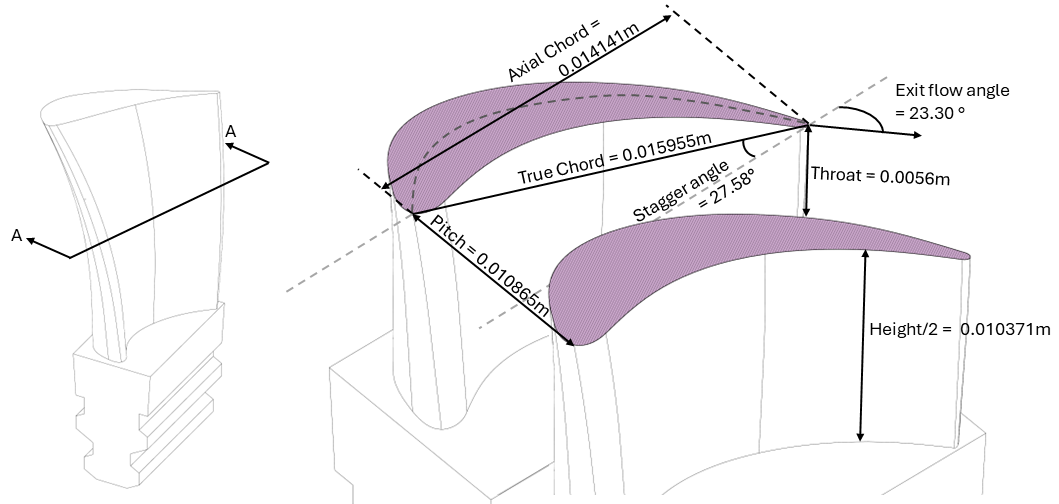
\includegraphics[width=0.99\linewidth]{figures/blade_detail_geom.png}
    \caption{Detail Blade Geometry}
    \label{fig:detail_blade_geom}
\end{figure}


\clearpage

\section{HPT Off-Design}
\subsection{HPT Off-Design Meanline Analysis}

 The off-design analysis begins, in which the blade speed is reduced by 10 percent (from 363.2 m/s to 326.9 m/s at the meanline), begins with the following assumptions:
\begin{itemize}
\item Assuming the mass flow rate is constant between on-design and off-design.
\item Assuming the vane exit properties are the same as in design conditions
\item Assume blade exit relative flow angle is the same as in design conditions (deviation = 0)
\end{itemize}

The table below summarizes the key off-design parameters.

\begin{table}[H]
    \centering
    \caption{Off-design Velocities and Angles}
    \begin{tabular}{|l|l|l|l|} \hline
        \multicolumn{2}{|c|}{\textbf{Stage 2}} & \multicolumn{2}{c|}{\textbf{Stage 3}} \\ \hline
        $\alpha_2$ & 69.35° & $\alpha_3$ & 29.91° \\ \hline
        $\beta_2$ & 36.99° & $\beta_3$ & 58.98° \\ \hline
        $C_{a_2}$ & 172.06 & $C_{a_3}$ & 300.6 \\ \hline
        $V_{w_2}$ & 129.61 & $V_{w_3}$ & 499.79 \\ \hline
        $V_2$ & 215.41 & $V_3$ & 583.22 \\ \hline
        $C_2$ & 487.86 & $C_3$ & 346.77 \\ \hline
        $C_{w_2}$ & 456.51 & $C_{w_3}$ & 172.89 \\ \hline
        $U_{OD}$& 326.9 & $U_{OD}$& 326.9 \\ \hline
    \end{tabular}
\end{table}

The image below shows the off-design velocity triangles compared with the on-design triangles. Note that the orange-dotted triangles are the design point triangles. 

\begin{figure}[H]
\centering
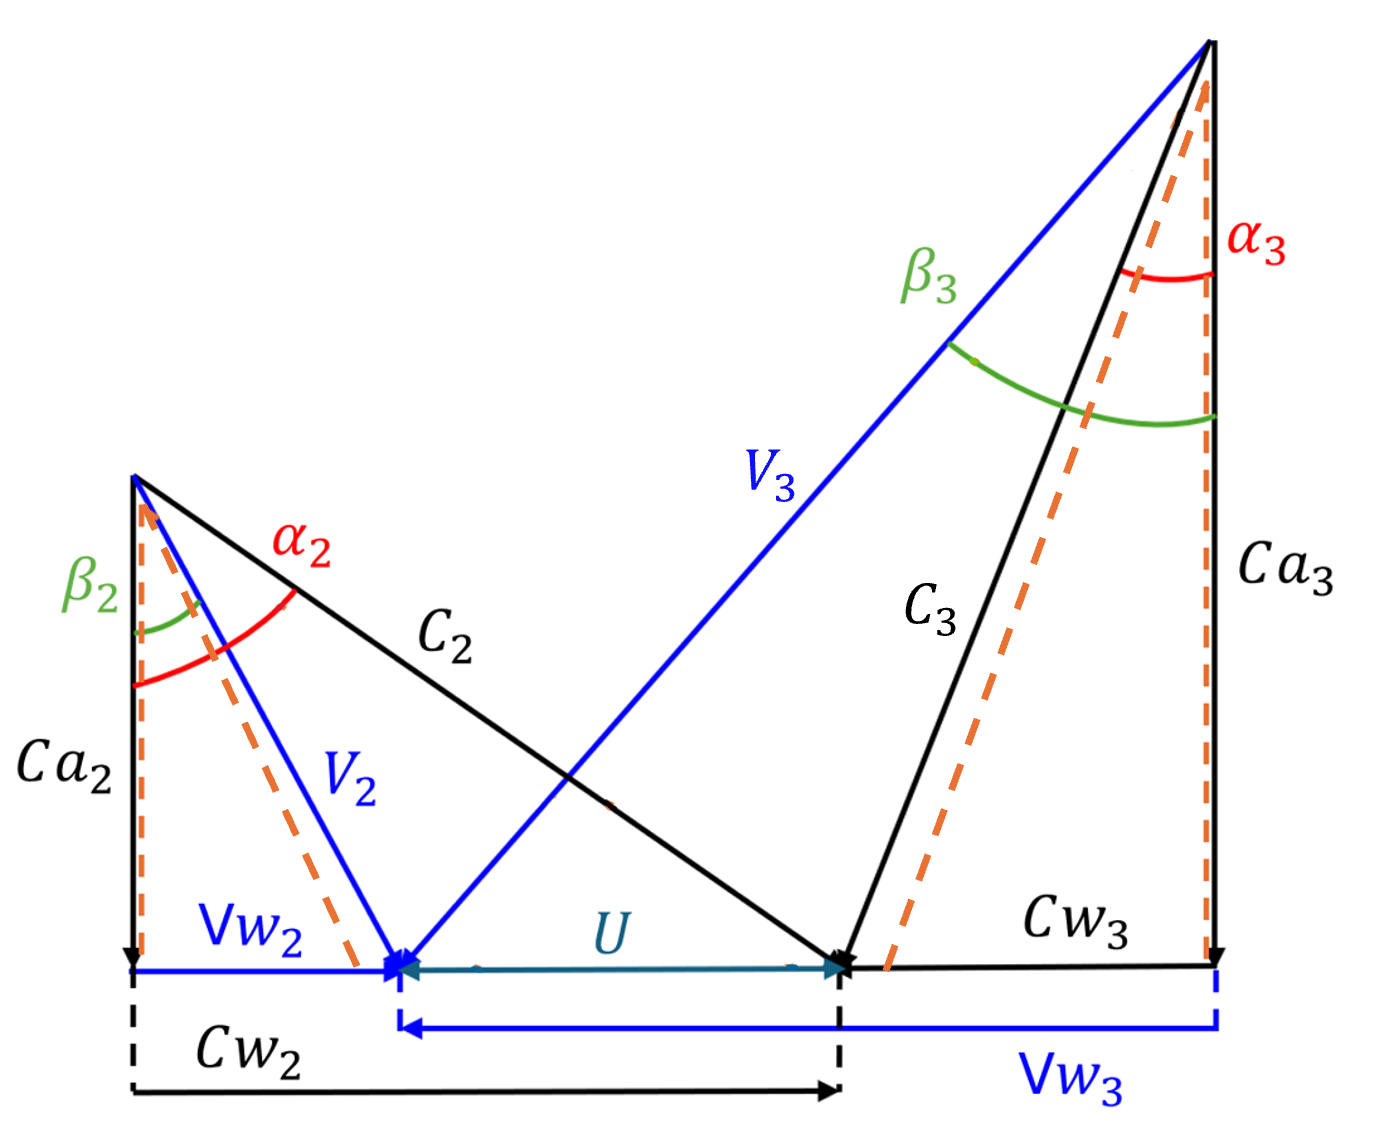
\includegraphics[width=0.5\textwidth]{figures/od_triangles.png}
\caption{Off-design and On-design velocity triangles}
\end{figure}

In addition, the off-design pressures, temperatures, work and incidence are shown in the table below for the exit. 

\begin{table}[H]
\centering
\caption{Off-design gas properties and incidence}
\begin{tabular}{|l|l|}
\hline
$T_{3,od}$ & 988.9 K\\ \hline
$T_{03,od}$ & 1041.3 K\\ \hline
$P_{3,od}$ & 421.32 kPa\\ \hline
$\rho_{3,od}$ & 1.48 $kg/m^3$\\ \hline
$W_{od}$ & 205.7 $kJ/kg$\\ \hline
$M_{3,rel,od}$ & 0.948\\ \hline
$Incidence$ & 8.52 degrees\\ \hline
\end{tabular}
\end{table}

The Python code below shows how the off-design parameters in the tables above were computed. In short, $Ca_3$ is iterated until the final $Ca_3$ satisfies both the equation of state (ideal gas law) and the conservation of mass for the given conditions and known exit geometry. The "LHS" variable is derived from beginning with the ideal gas law, then substituting $\rho$ for $P/{RT}$. The LHS equation becomes the known constants of $\dot{m}$, the gas constant R and known exit area. The RHS of the equation is equal to $Ca_3 * P/{T}$ which are all ultimately functions of $Ca_3$ as shown in the code. Therefore, by iterating $Ca_3$ until the RHS and LHS of the equations are in agreement (within some tolerance), then both the equation of state and conservation of mass are satisfied.
\clearpage
\begin{figure}[H]
    \begin{minted}[frame=lines, fontsize=\footnotesize,linenos]{python}
class off_design():   
    def calc_off_design(A_3, U_mean,beta_3,Ca_2, Cw_2, beta_2, a_2, a_3):
        U_mean_od = U_mean *0.9
        C_w_2_od = Cw_2
        flow_coeff_2_od = Ca_2/U_mean_od
        V_w_2_od = Cw_2 - U_mean_od
        beta_2_od = np.arctan(V_w_2_od/Ca_2)
        beta_2_od_deg = np.rad2deg(alpha_2_rel_od)
        incidence_2 = alpha_2_rel_od_deg - beta_2 
        v_2_od = np.sqrt(V_w_2_od**2 + Ca_2**2) 
        M_2_rel_od = v_2_od / a_2 
        T_2 = a_2**2/(gamma_g*R*1000)
        LHS = R*m_dot_3/A_3
        error_threshold = LHS * 0.01 #1 percent error of the LHS
        Ca_3_range = np.linspace(100,400,1000)
        Ca_3_od = 0
        for i in Ca_3_range:
            V_w_3_od = i * np.tan(np.deg2rad(beta_3))
            C_w_3_od = V_w_3_od - U_mean_od
            C_3_od = np.sqrt(i**2 + C_w_3_od**2)
            T_3_od = T_03 - (C_3_od**2)/(2*1000*c_p_gas)
            P_3_od = P_03 * (T_3_od/T_03)**(gamma_g/(gamma_g-1))
            RHS = i *P_3_od/T_3_od
            a_3_od = math.sqrt(gamma_g*R*1000*T_3_od)
            if np.abs(LHS - RHS) < error_threshold:
                Ca_3_od = i
                alpha_3_od = np.rad2deg(np.arctan(C_w_3_od/Ca_3_od))
                rho_3_od = P_3_od/(R*T_3_od)
                work_od_cw = U_mean_od*(C_w_3_od + C_w_2_od)
                work_od_vw = U_mean_od*(V_w_3_od + V_w_2_od)
                flow_coeff_3_od = Ca_3_od/U_mean_od
                V_3_od = np.sqrt(V_w_3_od**2 + Ca_3_od**2)
                M_3_rel_od = V_3_od/a_3_od
                # For physics check
                P_2 = P_3_od * ((T_2/T_3_od) ** (gamma_g/(gamma_g - 1)))
                P_02_rel = P_2*(1+ (gamma_g-1)/2 * M_2_rel_od**2)**(gamma_g/(gamma_g-1))
                P_03_rel = P_3_od*(1+ (gamma_g-1)/2 * M_3_rel_od**2)**(gamma_g/(gamma_g-1))
                break
            return T_3_od, rho_3_od, P_3_od, alpha_3_od, beta_2_od_deg, flow_coeff_2_od, 
            incidence_2, v_2_od, C_w_3_od,Ca_3_od,U_mean_od,flow_coeff_3_od, work_od_cw,
            work_od_vw, M_2_rel_od, M_3_rel_od, P_02_rel, P_03_rel
    \end{minted}
    \caption{Code snippet for calculating turbine hub properties.}
    \label{fig:code_turbine_hub}
\end{figure}

The following subsection outlines the losses that result from the 8.52 degrees of incidence observed above. 

\subsection{HPT Off-design Losses}

The same procedure as for the meanline design is used in terms of losses, such as finding the profile, secondary, trailing edge and tip clearance losses. Because trailing edge and tip clearance losses are calculated using the same equations as for on-design, only the profile and secondary losses calculations are shown. Throughout this section, snippets of code are attached to each loss to showcase and explain the design process.

For profile losses, \autoref{fig:code_turbine_hub} shows the code used to find the profile losses for off-design. Firstly, the following \autoref{eq:phi_squared_p0} was used to find the necessary correlation variables to find profile loss:

\begin{equation}
\label{eq:phi_squared_p0}
\phi_{P0}^2 = \frac{1}{1 + \frac{K_{P0}}{K_1 + K_2 K_{P0}}}
\end{equation}

In the meantime, Figure 2.34 from reference \cite{moustapha2003} was used to get the 2nd constant needed for the profile loss correlation formula. In that graph, the x-axis is represented by this \autoref{eq:figure2.34}:

\begin{equation}
\label{eq:figure2.34}
\left(\frac{d}{s}\right)^{-1.6} \left(\frac{\cos\beta_{1b}}{\cos\beta_{2b}}\right)^{-2} \left(\beta_1 - \beta_{1,\text{des}}\right)
\end{equation}

Once both values were found, $\phi$-squared could now be calculated with \autoref{eq:phi_squared_p}:

\begin{equation}
\label{eq:phi_squared_p}
\phi_P^2 = \phi_{P0}^2 - \phi_{\text{INC} - P}^2
\end{equation}

Finally, the last step is to plug the latter into the off-design profile loss \autoref{eq:K_p_od}:

\begin{equation}
\label{eq:K_p_od}
K_p = \frac{K_1(1 - \phi_p^2)}{\phi_p^2 - K_2(1 - \phi_p^2)}
\end{equation}

\begin{figure}[H]
    \begin{minted}[frame=lines, fontsize=\footnotesize,linenos]{python}
def off_design_k_p(inputs):
        phi_squared_P0 = 1 / (1 + ((K_p_rotor) / (K_1_rotor + K_2_rotor * K_p_rotor)))
        s = pitch_chord_ratio_rotor * c_true
        d_s = LE_diameter_rotor/s 
        graph_x = (d_s)**(-1.6) * (np.cos(np.radians(beta_2)) / 
        np.cos(np.radians(beta_3)))**(-2) * (np.radians(incidence))

        def figure_2_34(graph_x):
            fig_2_34 = pd.read_csv(r'_input_database\figure_2_34.csv')
            x = fig_2_34['graph_x'].values
            y = fig_2_34['deg_of_accel'].values

            interp_func = interp1d(x, y, kind='cubic')
            interpolated_y = interp_func(graph_x)

            return interpolated_y
        deg_of_accel = figure_2_34(graph_x)
        phi_squared_P = phi_squared_P0 - deg_of_accel
        K_p_od = (K_1_rotor * (1-phi_squared_P)) / (phi_squared_P - K_2_rotor *
        (1-phi_squared_P))
    \end{minted}
    \caption{Code snippet for calculating off design primary losses}
    \label{fig:code_turbine_hub}
\end{figure}

Afterwards, for the secondary losses, the process was simpler, where a ratio of the design and off-design secondary losses was obtained through the figure 2.35 from the reference \cite{moustapha2003}. Once that was done, the rest of the procedure was simply interpolating the various data points to optimize for the best value, which is outlined in the snippet of code of \autoref{fig:code_od_ks}.





\begin{figure}[H]
    \begin{minted}[frame=lines, fontsize=\footnotesize,linenos]{python}
def off_design_k_s(inputs):
        d_c = LE_diameter_rotor/c_true
        graph_x_2 = (d_c)**(-0.3) * (np.cos(np.radians(beta_2)) / 
        np.cos(np.radians(beta_3)))**(-1.5) * ((np.radians(incidence))/(np.radians(beta_2) 
        + np.radians(beta_3)))
        if graph_x_2 < 0.27:
            def figure_2_35(graph_x_2):
                fig_2_35 = pd.read_csv(r'_input_database\figure_2_35.csv')
                x = fig_2_35['x'].values
                y = fig_2_35['K_K_des'].values
                interp_func = interp1d(x, y, kind='cubic')
                interpolated_y = interp_func(graph_x_2)
                return interpolated_y
            
            K_K_des = figure_2_35(graph_x_2)
            K_s_od =  K_K_des * K_s_rotor
    \end{minted}
    \caption{Code snippet for calculating off design secondary losses.}
    \label{fig:code_od_ks}
\end{figure}

Afterwards, the trailing edge losses and tip clearance losses were calculated using the same method as on-design meanline aerodynamic losses, where trailing edge losses permitted to output all the various blade geometry features, and tip clearance allowed to calculate the final efficiency following the decrease from aerodynamic losses. Once those same calculations were done for the rest of the off-design losses, the new off-design total-to-total efficiency was calculated, showing how much the off-design was affected by it. The final off-design efficiency for this design holds at a 87.21\%, following the addition of a -4 degree incidence. For all the efficiency values extracted from this process and outputted from the code, see \autoref{tab:calculated_design_efficiencies}





\section{Efficiency Calculation}

The following table, \autoref{tab:calculated_design_efficiencies} compiles all the calculated efficiencies, including total-to-total and final efficiencies for both on design and off-design parameters:

\begin{table}[ht]
\centering
\caption{Calculated Design Efficiencies}
\label{tab:calculated_design_efficiencies}
\begin{tabular}{|l|l|l|}
\hline
\textbf{Efficiency}                 & \textbf{Value} & \textbf{Comments}\\ \hline
$\eta_{tt}$                & 90.26 \% &    Turbine total-to-total efficiency     \\ \hline
$\eta_{final}$             & 88.50 \% &    Final design efficiency     \\ \hline
$\eta_{final,od}$          & 86.96 \% &    Off design efficiency     \\ \hline
$\eta_{final,od,new}$      & 87.21 \% &    Off design efficiency after adding design incidence     \\ \hline
$\Delta\eta_{final}$       & 1.13 \% &    Off design efficiency drop    \\ \hline
\end{tabular}

\end{table}
\clearpage

%%%%%%%%%%%%%%%%%%%%%%%%%%%%%%%%%%%%%%%%%%%%%%%%%%%%%%%%%%%%%%%%%%%%%%%%%%%%%%%%%%%%%%%%%%
%               PART D             %
%%%%%%%%%%%%%%%%%%%%%%%%%%%%%%%%%%%%%%%%%%%%%%%%%%%%%%%%%%%%%%%%%%%%%%%%%%%%%%%%%%%%%%%%%%
\chapter{Trade Studies}
\section{Trade Study 1: Blade Material}

The selection of a turbine blade material is one which should be taken with great care. These materials must be able to withstand extremely high temperatures while also maintaining their structural integrity at extremely high rotational speeds. Due to these extremely harsh environments, chromium nickel alloys are often chosen. With their high strength and low density, along with its ease of manufacturing make it a favorite in the aerospace industry.

In this trade study, this alloy shall be used as a baseline material, and compared with materials that have similar thermal and stress characteristics, while having both higher and lower densities and varying lifespans. These differences will be used to calculate the impact on the cost to the consumer which shall be compared to the overall lifetime cost of an engine.

The materials used in the trade study will be shown as such: Material X shall be the baseline material. The baseline density of 0.296kg/m3 shall be used, along with characteristics such as melting point, yield stress, etc. This material has a Factory Standard Cost (FSC) of 150 USD and will be rated at 5000 hours of life capability. Material Y offers a cheaper solution, with an FSC of 125USD per blade, a 5 percent lower density, and a life capability of 4000 hours. Material Z is a more durable solution, offering an FSC of 175USD per blade, with a 5 percent higher material density, and a lifecycle capacity of 8000 hours. These values are also summarized in the table below.
\begin{table}[H]
\centering
\caption{Summary of Trade Study Materials}
\begin{tabular}{|c|c|c|c|}
\hline
\textbf{Material} & \textbf{FSC (USD)} & \textbf{Life Capability (hrs)} & \textbf{Density (to baseline)} \\ \hline
Material X        & \$150               & 5000                            & --                              \\ \hline
Material Y        & \$125               & 4000                            & -5\%                            \\ \hline
Material Z        & \$175               & 8000                            & +5\%                            \\ \hline
\end{tabular}

\end{table}

For each blade configuration, the number of overhauls required will also be calculated. The timing of an overhaul shall be determined by the turbine blade life capability outlined above. Each overhaul shall be estimated to cost the client 90,000USD. The number of total overhauls is assumed based on an estimated engine lifespan of 25,000 hours, with an average of 2,500 hours per year.

Further, an increase of 60 percent shall be added to the blade costs as a sale markup.
With this information, the total cost to the client has been calculated and tabled below.

\begin{table}[H]
\centering
\caption{Lifetime Cost per Engine}
\begin{tabular}{|c|c|c|c|}
\hline
                         & \textbf{Material X} & \textbf{Material Y} & \textbf{Material Z} \\ \hline
Sale Price, Blades (USD) & 9,300               & 7,750               & 10,850              \\ \hline
Lifetime Overhaul Cost** (USD) & 450,000          & 540,000             & 270,000             \\ \hline
Overhauls Required       & 5                   & 6                   & 3                   \\ \hline
\textbf{Total Cost (USD)} & \textbf{464,880}   & \textbf{552,400}   & \textbf{287,360}   \\ \hline
\end{tabular}

\end{table}

From the table above, although Material Z has a higher upfront cost, the lifetime cost savings are substantial. Further, with an overhaul taking time away from the working time of the aircraft, the operator’s losses due to the aircraft remaining stationary for weeks cannot be ignored. By having two less scheduled overhauls, the client will not only save over 180,000 USD, but gain weeks of usable time for their aircraft. Unfortunately, the cost of choosing Material Z is an increase in weight of 5 percent. To help reduce this weight increase, another trade study was conducted to reduce the engine weight. 

\section{Trade Study 2: Weight Reduction}

As with any element of an aircraft, the engine shall be designed with weight considerations in mind. As such, a trade study to reduce the engine weight has been conducted. To reduce the weight, an attempt at increasing the engine efficiency has been made. To increase the efficiency, the peak cycle temperature can be increased, resulting in a decrease in specific fuel consumption (SFC). While keeping the output power of the engine the same, a lower volume of fuel should be needed, leading to a reduction in weight. This reduction in fuel weight should also save the operator in running costs, as the engine becomes more fuel efficient.

To accommodate for the increase in temperature, additional cooling shall be provided to the HPT such that for every 100°F of increase, cooling increases 1 percent from baseline. This will in turn reduce the HPT efficiency by 0.2 percent. The primary reduction in weight would focus on the amount of fuel consumed by the engine, as with an increase in peak temperature causing an increase in efficiency, less fuel consumption will occur. 

The increases in temperature were chosen to be ever 100°F up until approximately 2000°F as this was to be considered the design limit of the material, while considering the extra cooling. These initial points were split further to allow for more detailed analysis, adding four points between each temperature. This led to a total of 12 data points for consideration. Due to the large processing time associated with this computation, the solution was not refined further. 

By inserting the various temperatures into the Python script, the engine SFC, and air-to-fuel ratio are output given the power output remains constant. This then allows for the fuel consumption to be calculated, which will then demonstrate the decrease in weight due to fuel. The tabulated data for the key points of increases of 100°F is shown below.

\begin{table}[H]
\centering
\caption{Results of Increasing Peak Cycle Temperature}
\begin{tabular}{|c|c|c|c|c|}
\hline
\textbf{Peak temp (K)} & \textbf{SFC} & \textbf{Fuel to air ratio} & \textbf{Fuel Operational Cost (USD/hr)} & \textbf{Fuel weight (lbs)} \\ \hline
1245                    & 0.41761      & 0.2                         & 402.52                                 & 751.38                     \\ \hline
1301                    & 0.36369      & 0.017416                    & 350.55                                 & 654.36                     \\ \hline
1357                    & 0.32323      & 0.015478                    & 311.56                                 & 581.57                     \\ \hline
\end{tabular}

\end{table}

From this analysis, a sharp decrease in the fuel consumption per hour can be observed. With the rising cost of fuel and companies continually being required to lower emissions, this could prove as a vital selling point of the engine. This in turn means that 169.81 lbs can be saved for every hour of flight, proving to also be economical in terms of the weight of the propulsion system.

Furthermore, we may also reduce weight through other means. If the client deems the weight loss outweighs the significant cost increase for overhauls, a lighter material such as Material Y could be chosen. This however is not recommended, as the gains would be too few to warrant the cost. Alternatively, the turbine can be optimized to use the least number of blades possible. This would reduce the sale cost to the client, as well as save weight. However, the blades would be more highly loaded, but would still be within the acceptable range to maintain the promised life capability.

The result of the trade studies has allowed for a more cost efficient and marketable engine. Based on the conducted trade studies, the final recommendation is as follows:
\begin{enumerate}
    \item Select Material Z for the turbine blades: This material’s long-life capability proves that it is the most cost-effective option and the weight gain from choosing this option can be mitigated.
    \item Increase the peak cycle temperature to 1357K: Increasing the peak cycle temperature allows for a more fuel-efficient engine and saves weight on fuel.
    \item Reduce the blade count in the turbine: Reducing the number of blades in the rotor and stator of the turbine will keep the sale cost low for the client, while saving weight on engine design.
\end{enumerate}
\clearpage

%%%%%%%%%%%%%%%%%%%%%%%%%%%%%%%%%%%%%%%%%%%%%%%%%%%%%%%%%%%%%%%%%%%%%%%%%%%%%%%%%%%%%%%%%%
%               CONCLUSION             %
%%%%%%%%%%%%%%%%%%%%%%%%%%%%%%%%%%%%%%%%%%%%%%%%%%%%%%%%%%%%%%%%%%%%%%%%%%%%%%%%%%%%%%%%%%
\chapter{Conclusion}

To conclude this technical report, the optimization process for the gas turbine engine design was presented with detailed sections for the cycle calculations, high pressure compressor, high pressure turbine, and finally the trade studies. In the cycle calculation the overall engine cycle was covered and afterwards, a detailed high pressure compressor design is shown, followed by an extensive high pressure turbine design. This included the meanline design, free vortex design, aerodynamic losses and finally the off-design parameters. Finally, the trade studies were presented in order to select an appropriate blade material and decrease the overall weight.

The turbine conforms to all constraints provided in the outline, and conforms to physics. The turbine design summarized in this paper is the result of an optimization process discussed previously and takes into account engine efficiency, efficiency drop during off-design operation, number of rotor blades and the structural limit of the blade (via $AN^2$).

\begin{table}[htbp]
\centering
\begin{tabular}{|c|c|}
\hline
\textbf{Column 1} & \textbf{Column 2} \\ \hline
$\eta_{final}$ & 88.50\% \\ \hline
$\eta_{off design}$ & 87.21\% \\ \hline
$AN^2$ & 1,819,183 \\ \hline
$M_{abs,exit}$ & 0.522 \\ \hline
$\alpha_{exit}$ & 23.30 degrees \\ \hline
$\omega$ & 4214.5 rad/s \\ \hline
\end{tabular}
\caption{Turbine Characteristics}
\label{tab:turbine_characteristics}
\end{table}

The compressor in turn functions within the given constraints, including a relative Mach number below 1, aspect ratio of the diffuser is between 0.8 and 1.2 and the relative (0.5 and 0.6) and axial velocity range (between 0.8 and 1).

By incorporating trade studies into the design process, a more refined, optimized solution was determined and this aims to reduce the cost and downtime of the engine to the client. By following the recommendations outlined in this report, the final design showcases an engine which proves to be competitive in an ever-growing market. 

\clearpage
%%%%%%%%%%%%%%%%%%%%%%%%%%%%%%%%%%%%%%%%%%%%%%%%%%%%%%%%%%%%%%%%%%%%%%%%%%%%%%%%%%%%%%%%%%
%               REFERENCES              %
%%%%%%%%%%%%%%%%%%%%%%%%%%%%%%%%%%%%%%%%%%%%%%%%%%%%%%%%%%%%%%%%%%%%%%%%%%%%%%%%%%%%%%%%%%
\bibliographystyle{plain}
\bibliography{refs}
\pagebreak


%%%%%%%%%%%%%%%%%%%%%%%%%%%%%%%%%%%%%%%%%%%%%%%%%%%%%%%%%%%%%%%%%%%%%%%%%%%%%%%%%%%%%%%%%%
%               SETS APPENDIX FORMATTING              %
%%%%%%%%%%%%%%%%%%%%%%%%%%%%%%%%%%%%%%%%%%%%%%%%%%%%%%%%%%%%%%%%%%%%%%%%%%%%%%%%%%%%%%%%%%
\appendix
\chapter*{APPENDICES}
Space left blank on purpose.
\addcontentsline{toc}{chapter}{Appendices}
\renewcommand{\chaptername}{Appendix} 
%%%%%%%%%%%%%%%%%%%%%%%%%%%%%%%%%%%%%%%%%%%%%%%%%%%%%%%%%%%%%%%%%%%%%%%%%%%%%%%%%%%%%%%%%%
%               END OF APPENDIX FORMATTING             %
%                 APPENDIX CONTENT BEGINS             %
%%%%%%%%%%%%%%%%%%%%%%%%%%%%%%%%%%%%%%%%%%%%%%%%%%%%%%%%%%%%%%%%%%%%%%%%%%%%%%%%%%%%%%%%%%


\chapter{Python Script} \label{sec:app_output}
Space left blank on purpose.
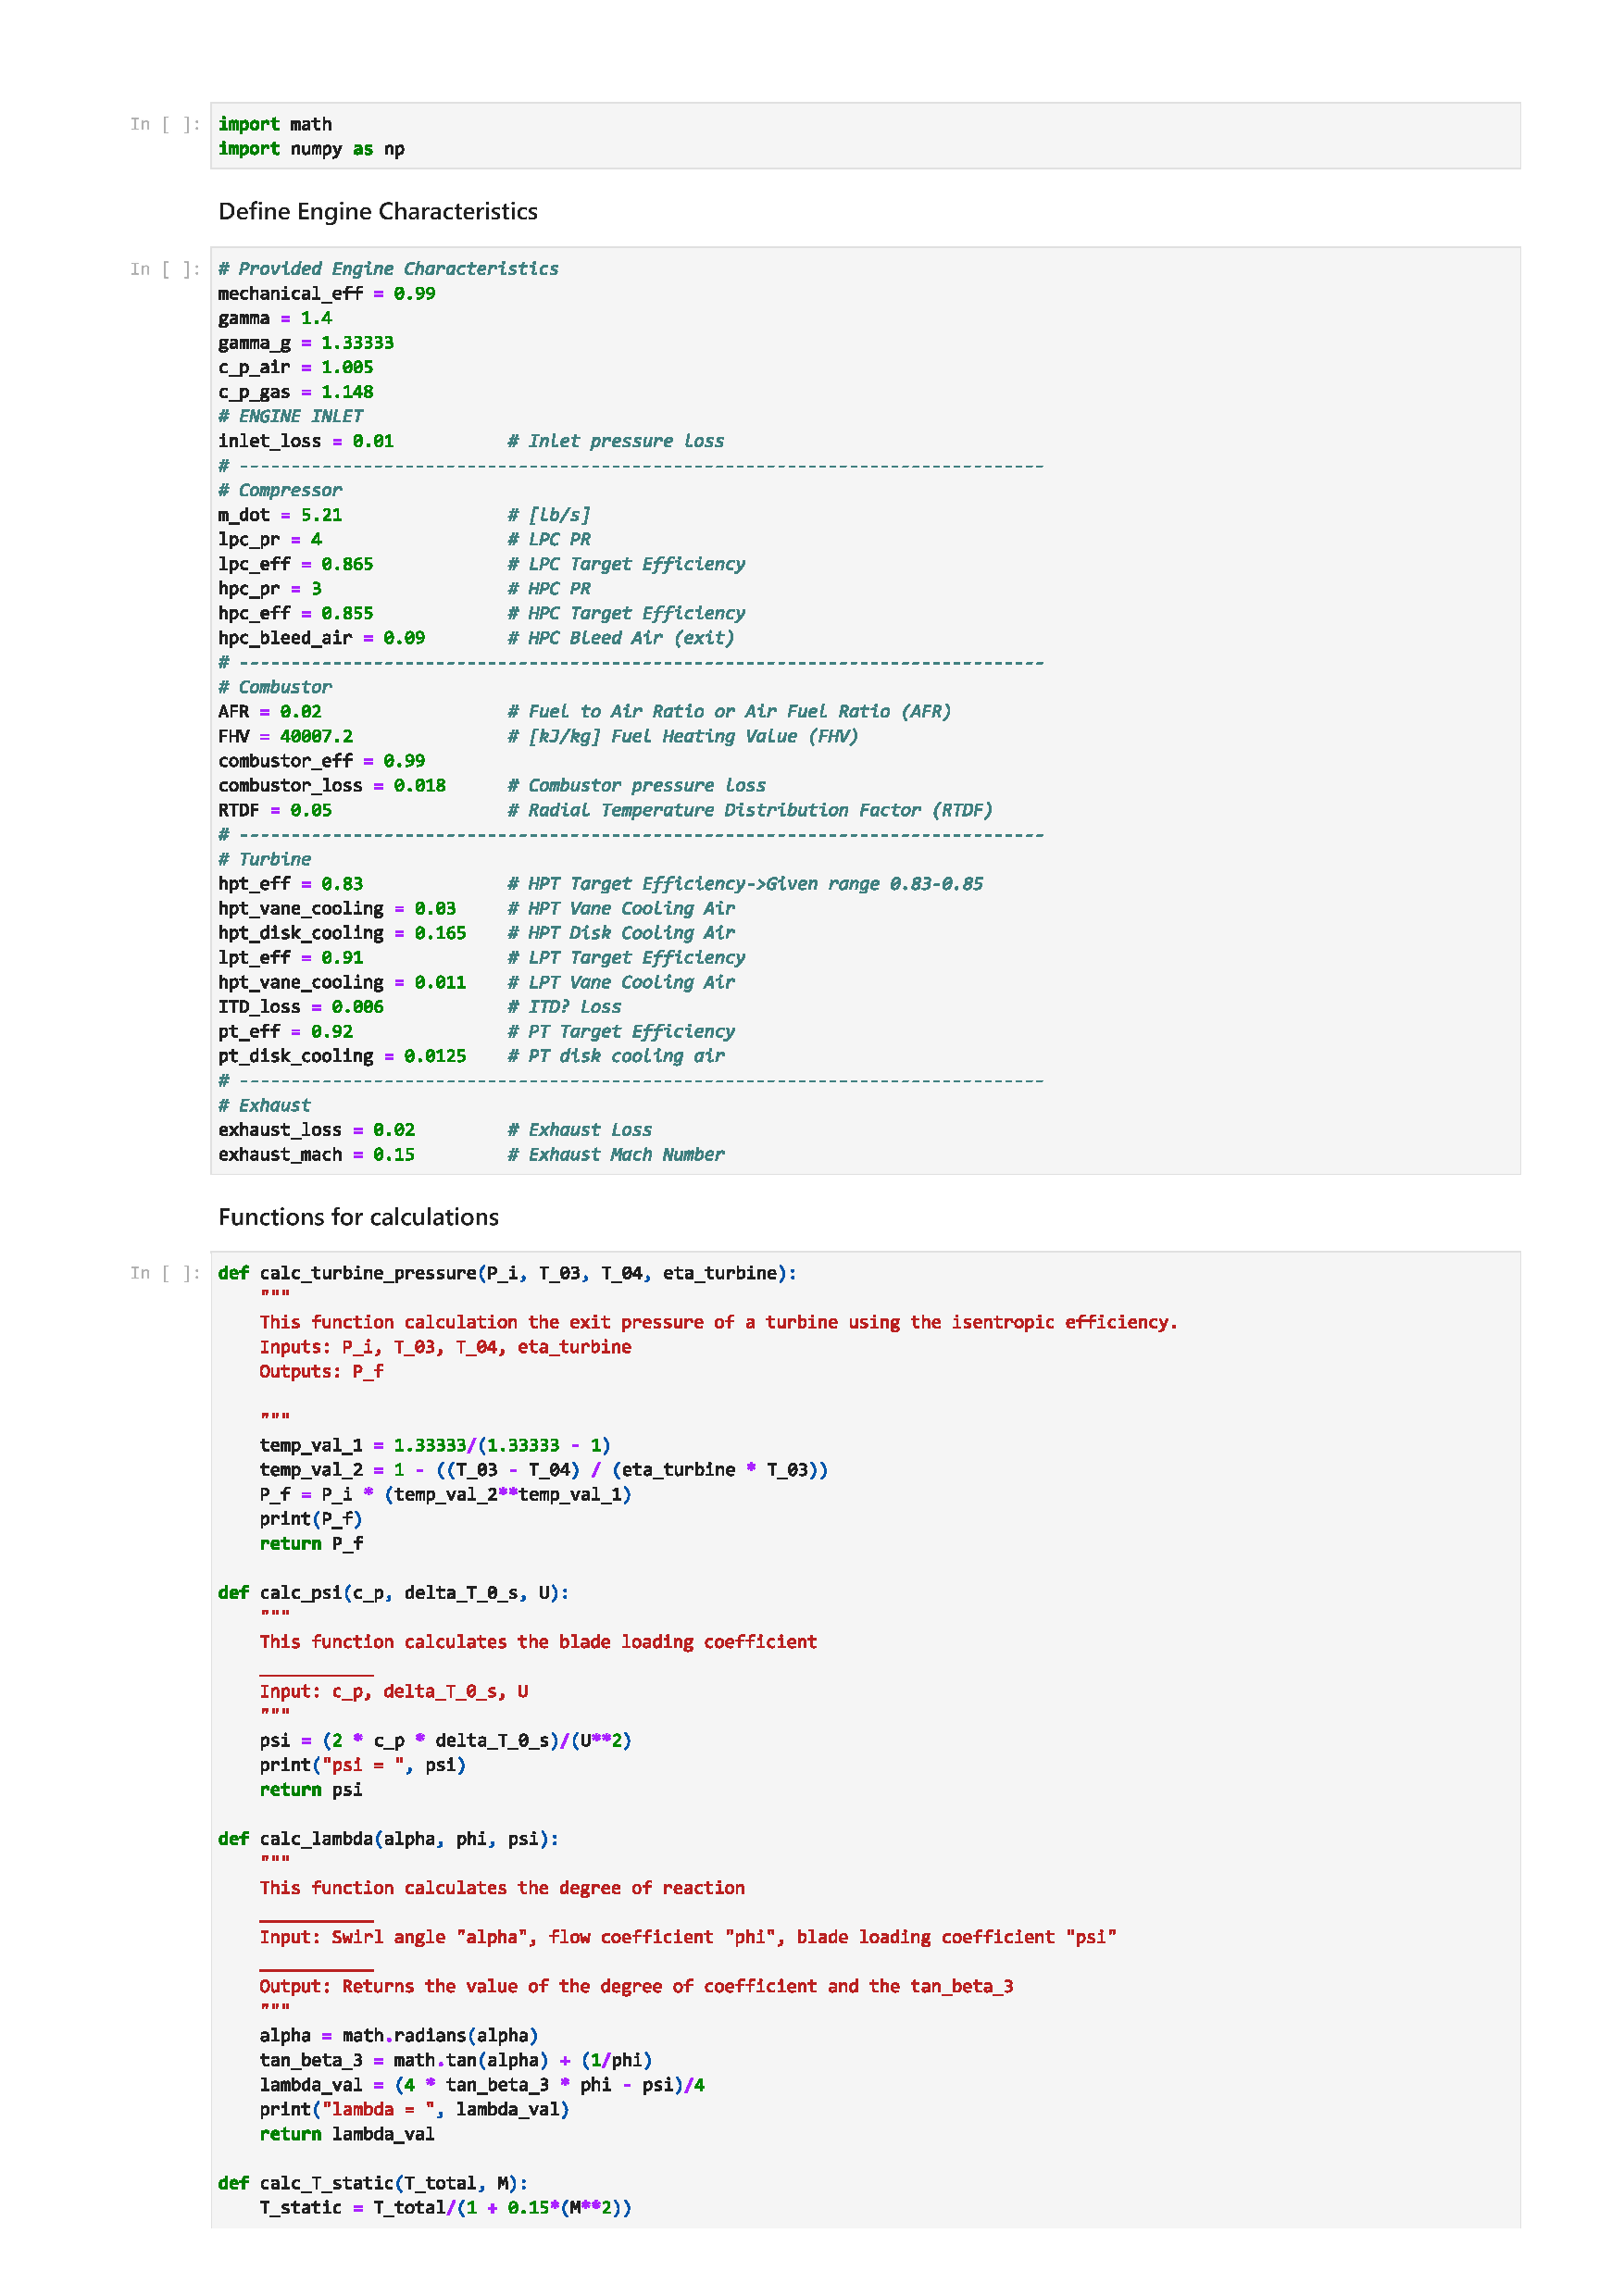
\includepdf[pages=-]{attachments/app.pdf}


\chapter{HPT Calculation Functions}
Space left blank on purpose.
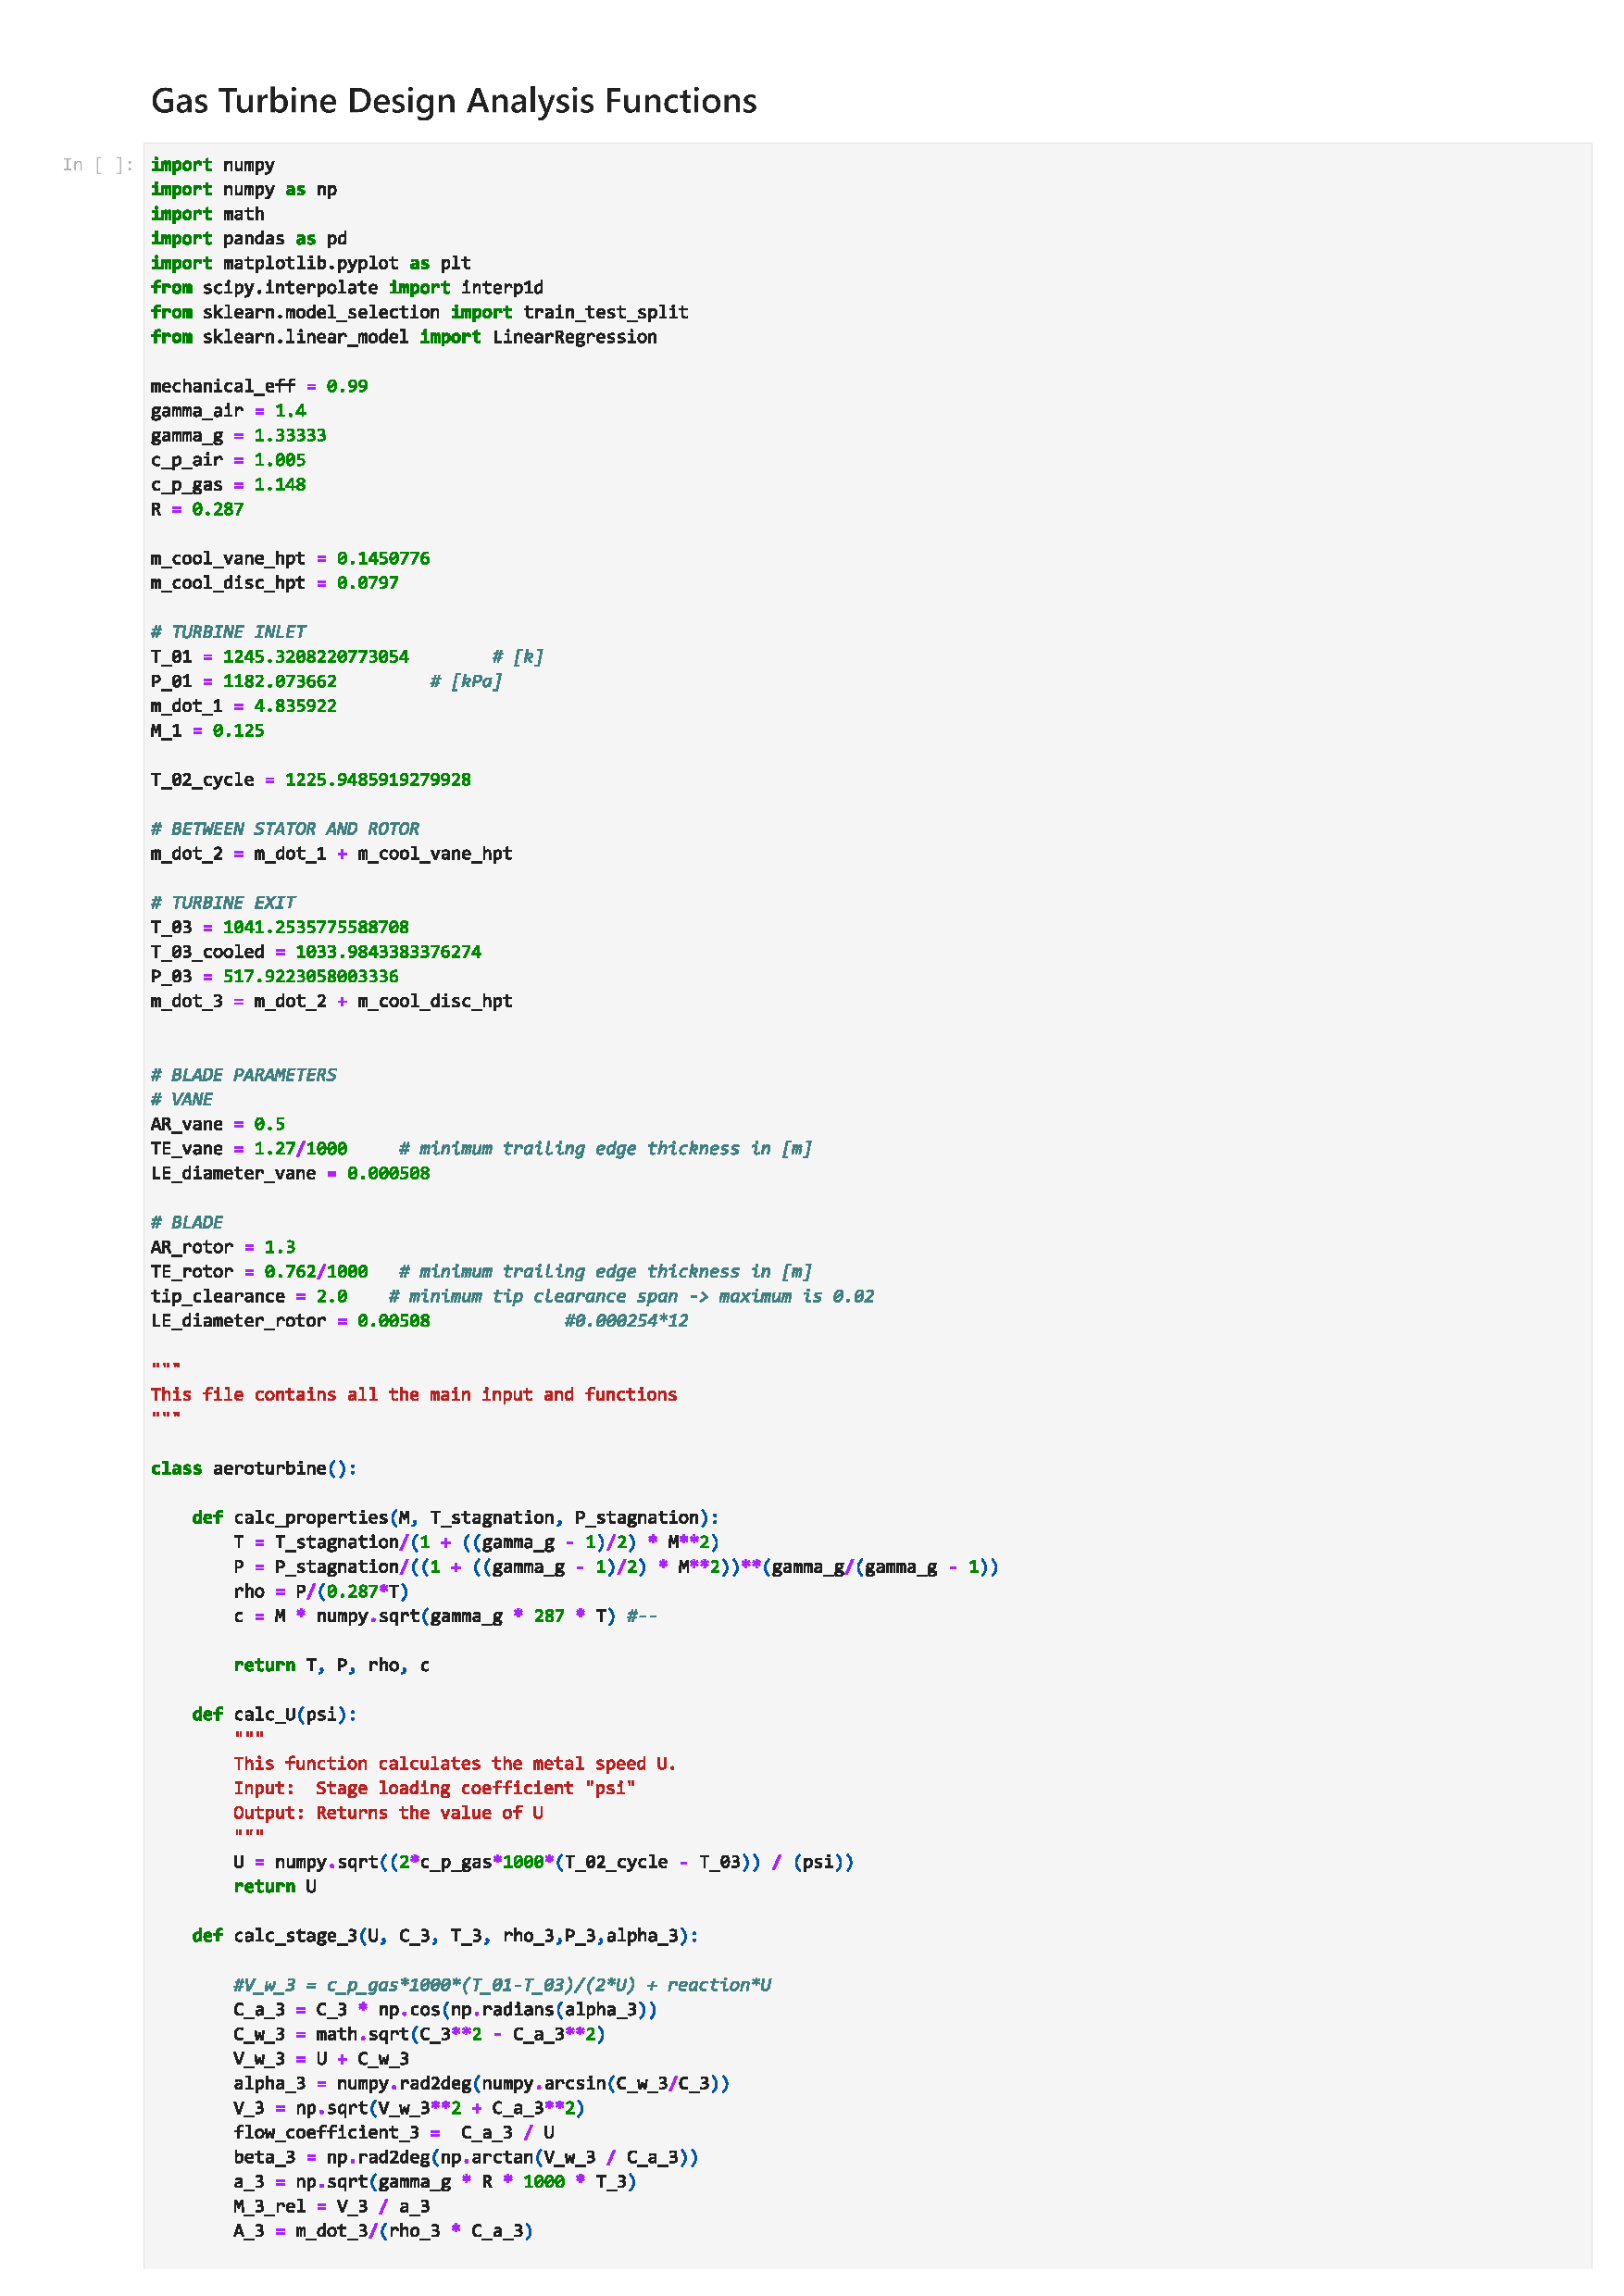
\includepdf[pages=-]{attachments/functions_pdf.pdf}

\chapter{HPT Calculation Loop}
Space left blank on purpose.
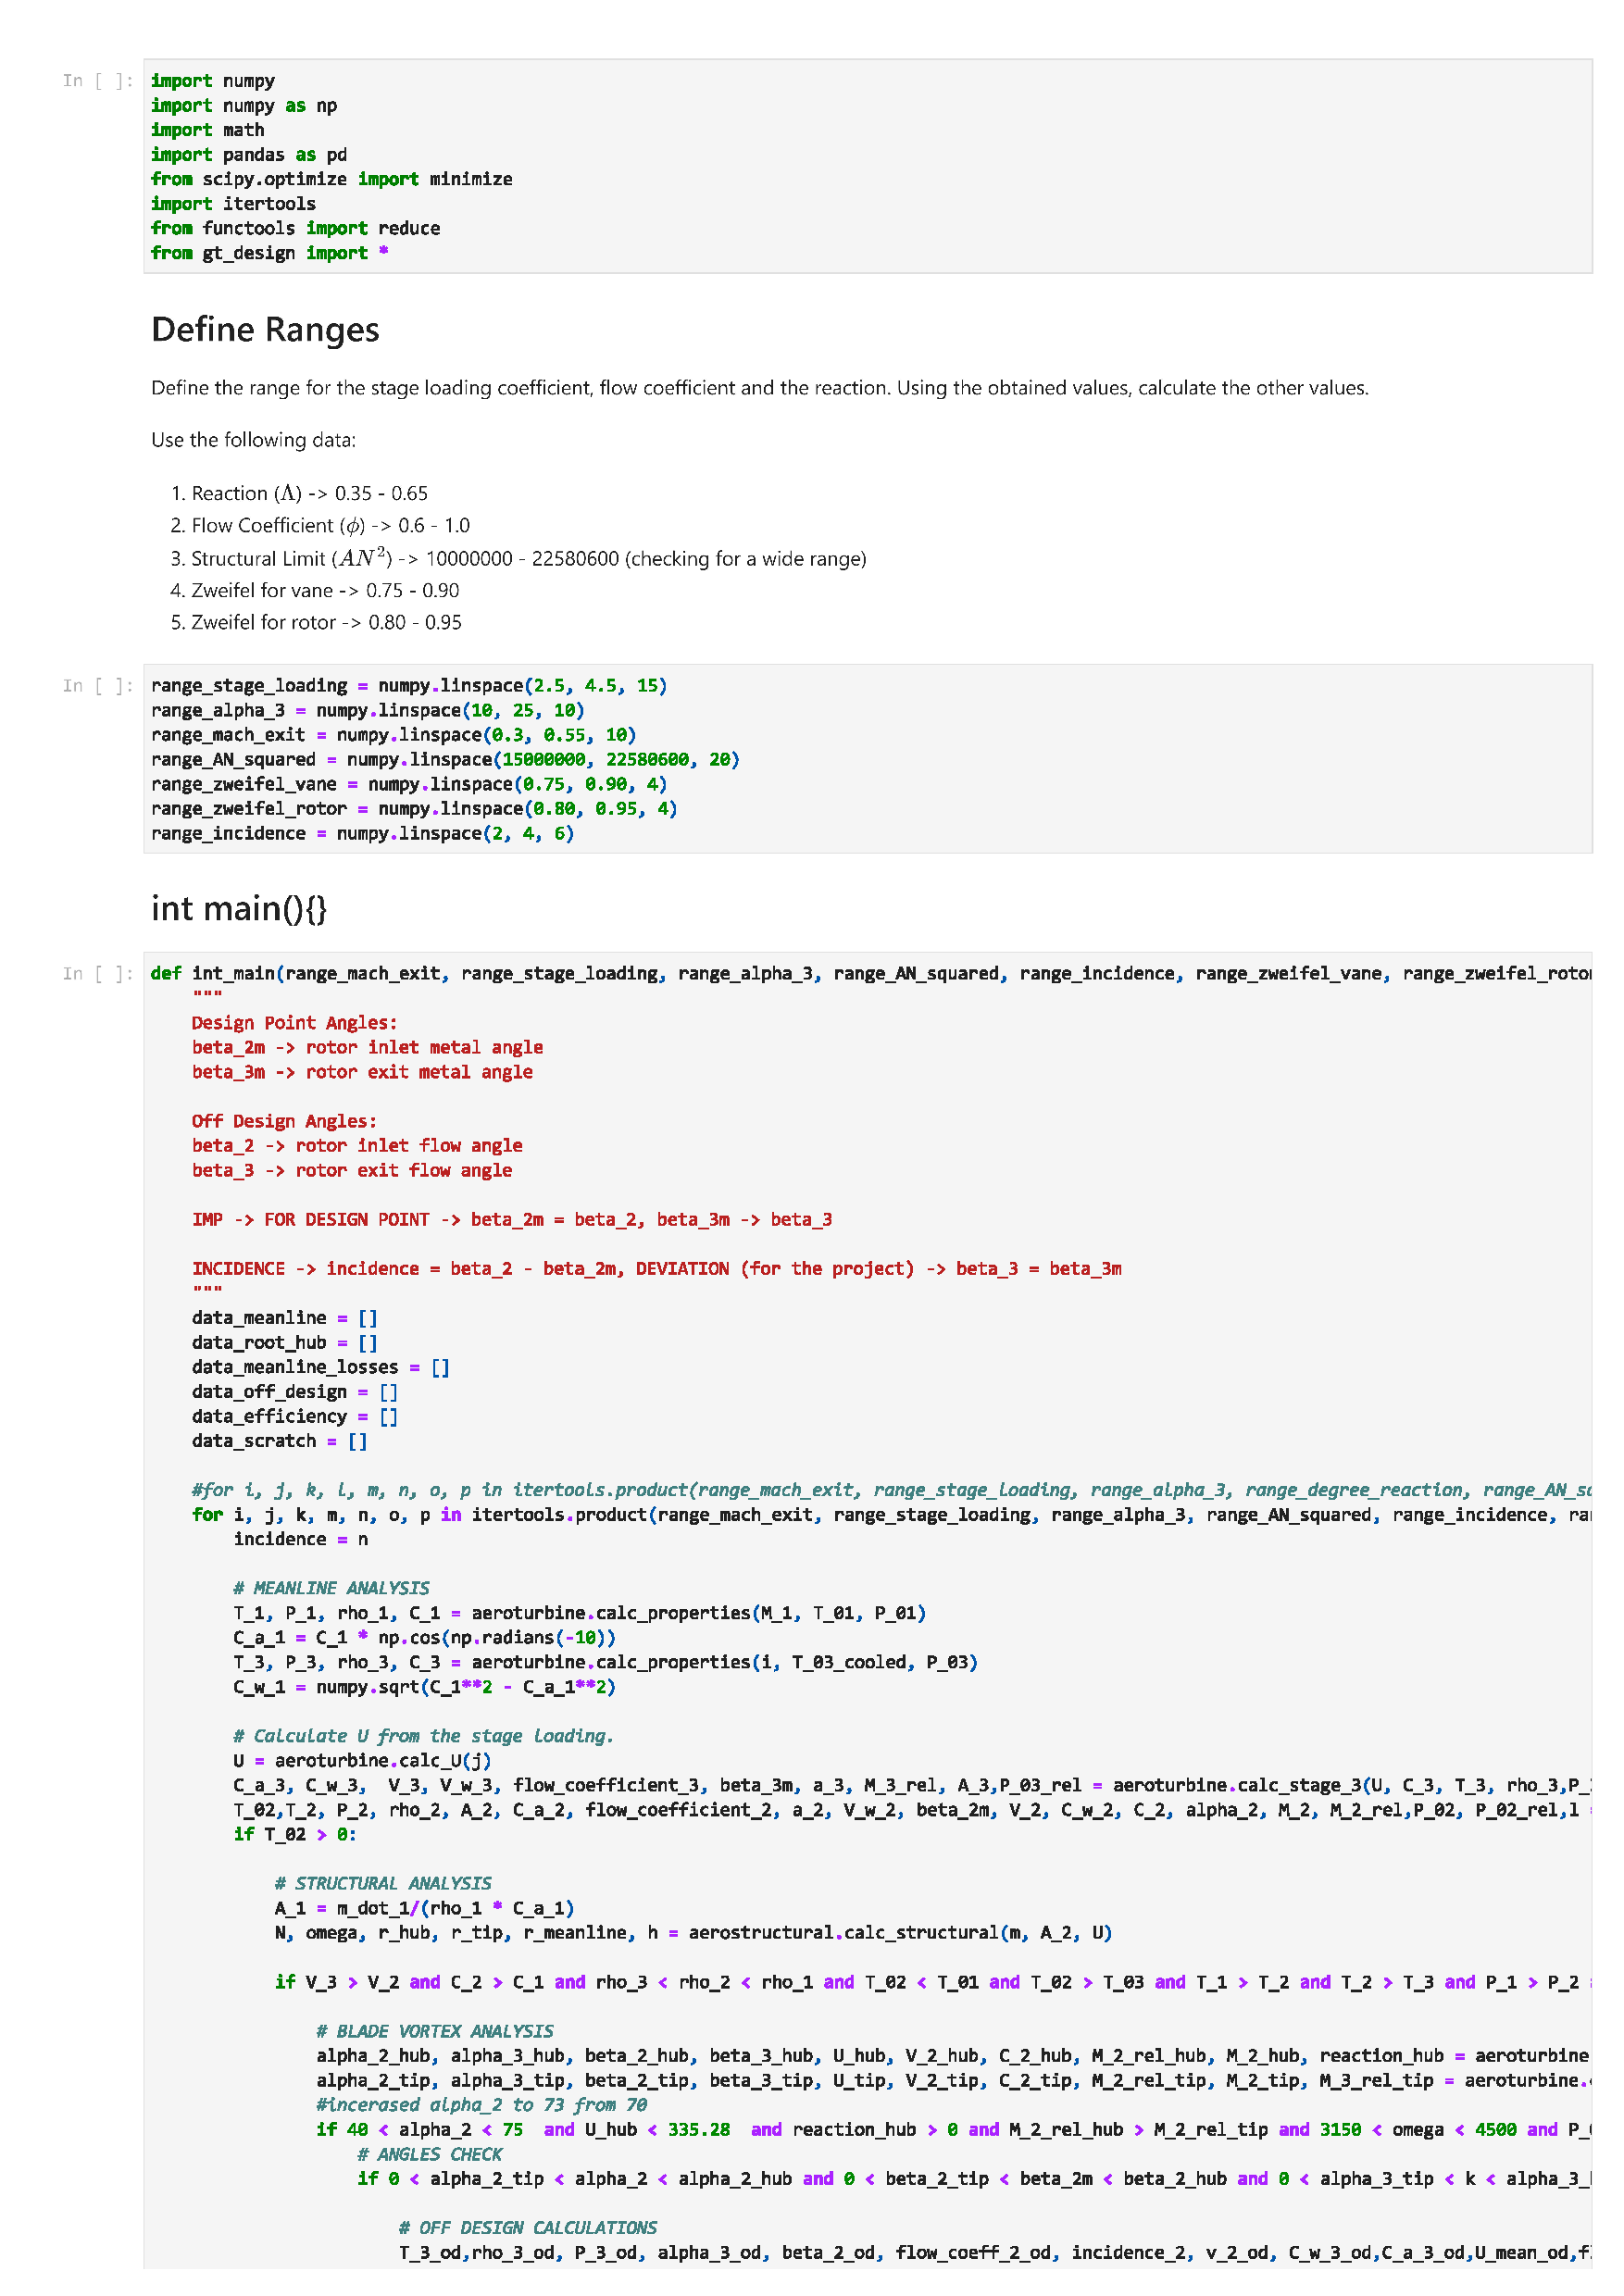
\includepdf[pages=-]{attachments/true_stories.pdf}


\end{document}